\section{Carcharhiniformes}\index{Carcharhiniformes}

\subsection{Carcharhinidae}\index{Carcharhinidae}\index{Carcharhiniformes!Carcharhinidae}

\subsubsection{Carcharhinus acronotus - Blacknose shark}\index{Blacknose shark}\index{Carcharhinus acronotus}\index{Carcharhinidae!Carcharhinus acronotus}
\begin{center}
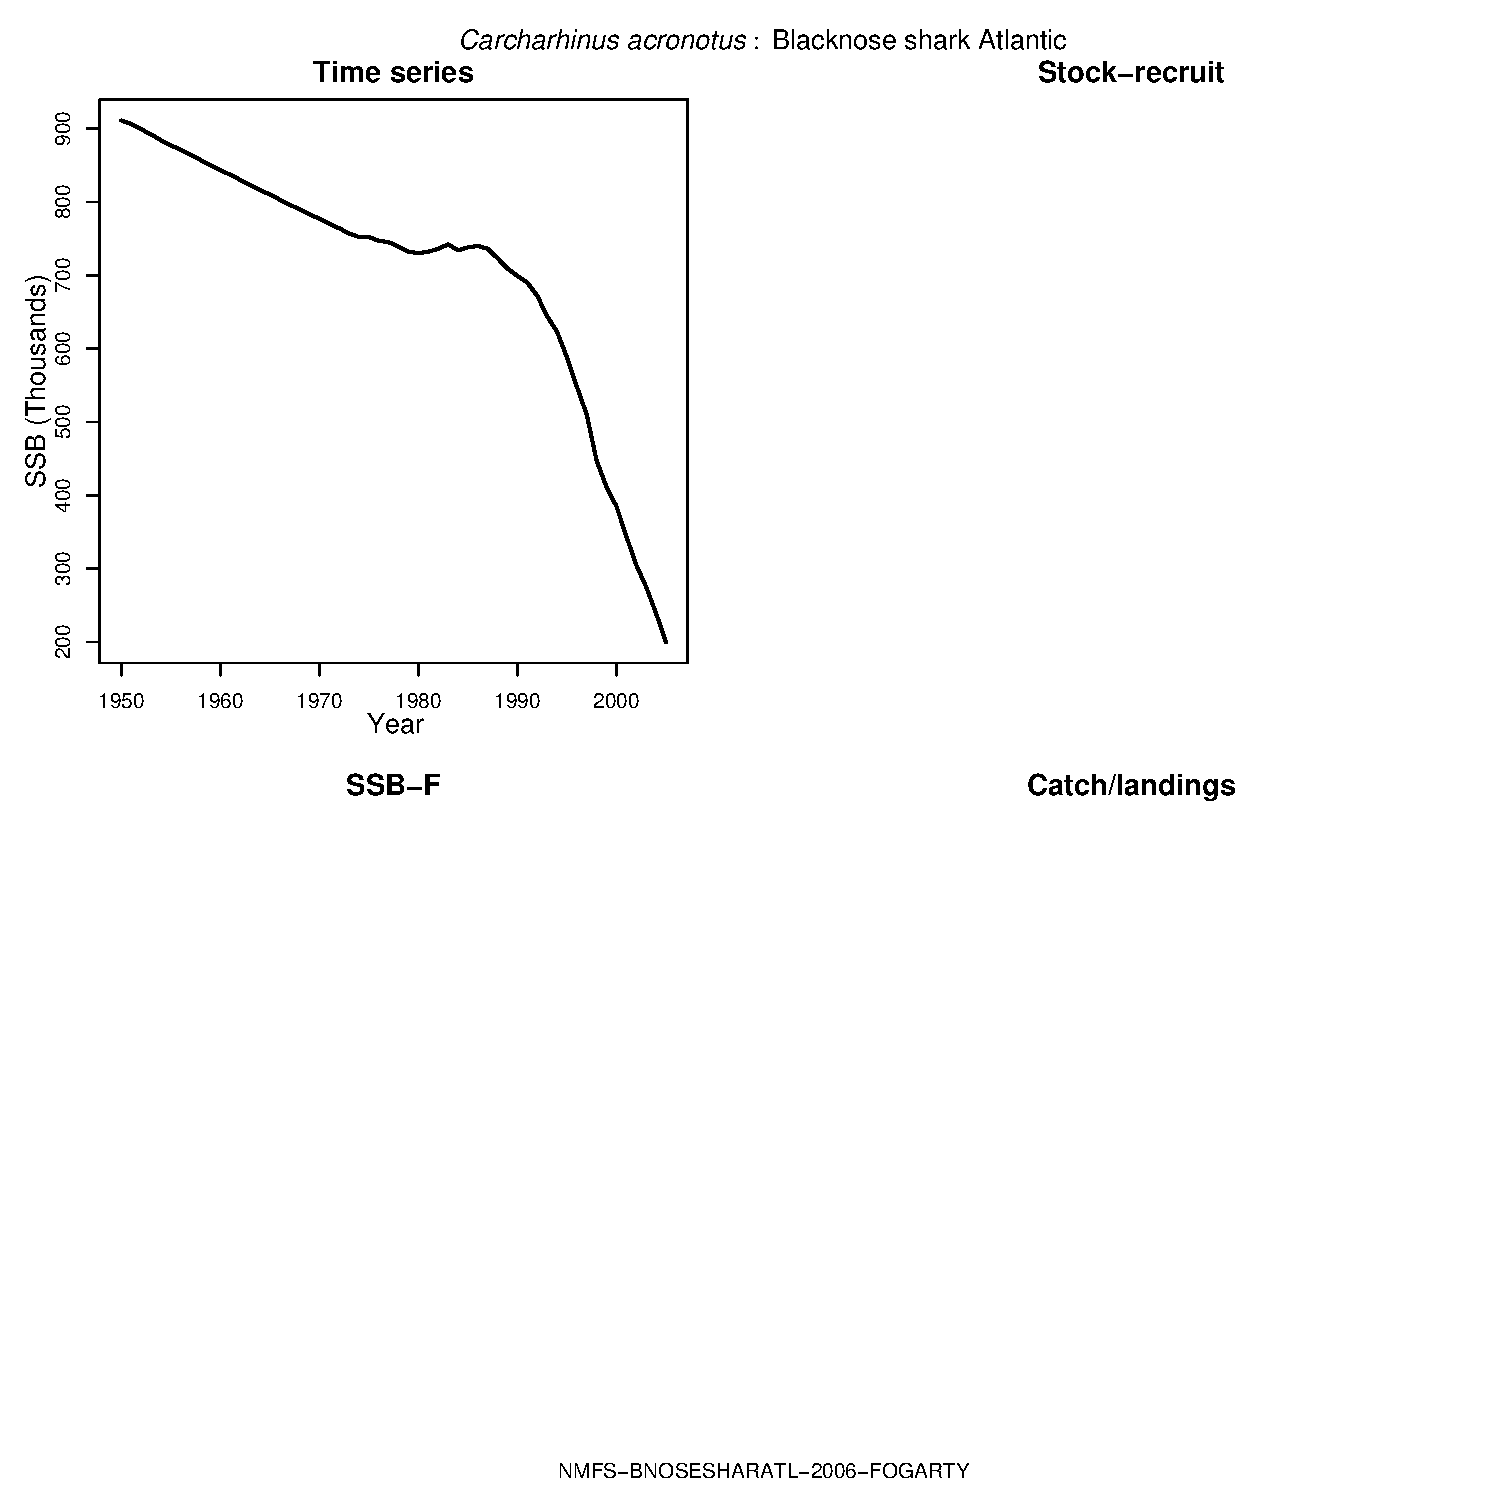
\includegraphics[width=1.2\textwidth]{../R/figures/NMFS-BNOSESHARATL-2006-FOGARTY.pdf}
\end{center}

\subsubsection{Carcharhinus limbatus - Blacktip shark}\index{Blacktip shark}\index{Carcharhinus limbatus}\index{Carcharhinidae!Carcharhinus limbatus}
\begin{center}
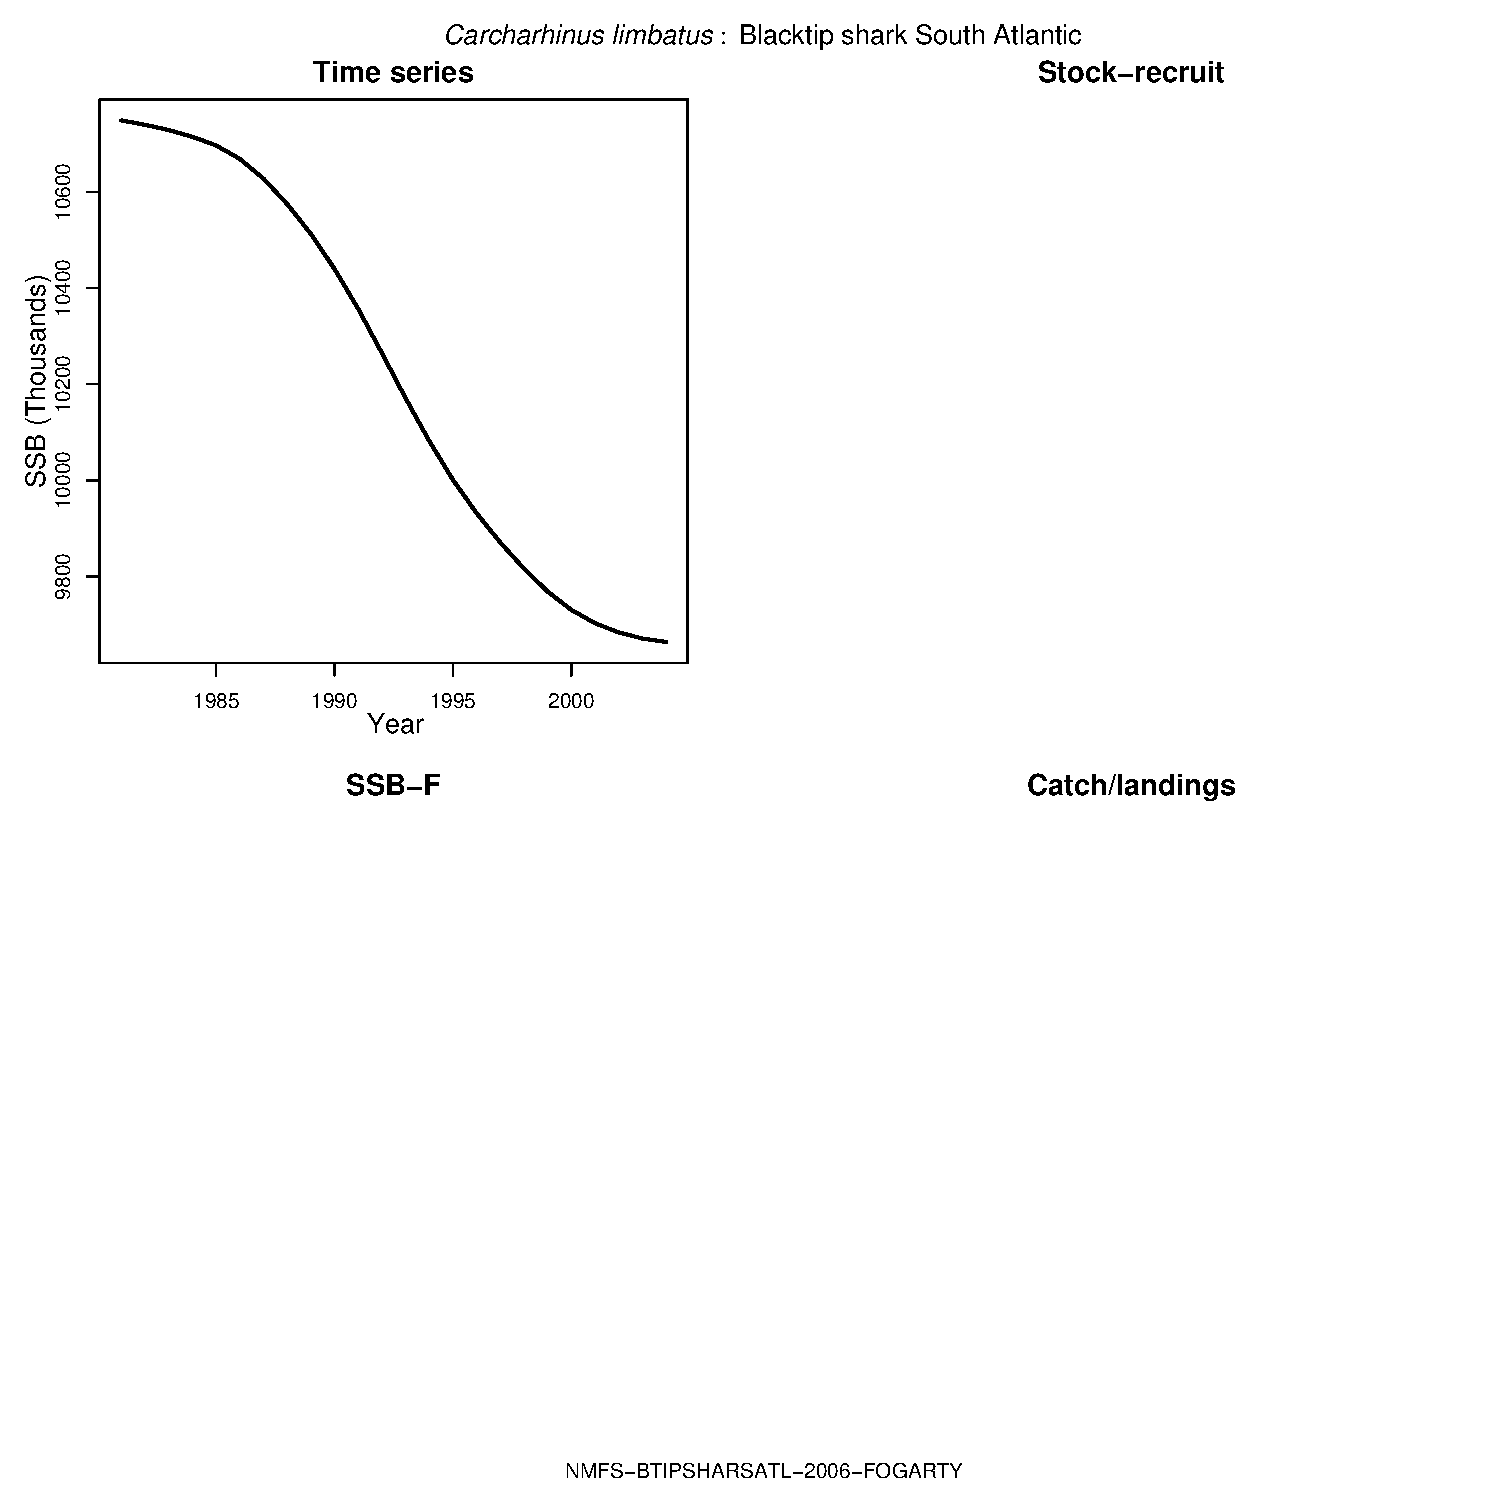
\includegraphics[width=1.2\textwidth]{../R/figures/NMFS-BTIPSHARSATL-2006-FOGARTY.pdf}
\end{center}

\subsubsection{Carcharhinus plumbeus - Sandbar shark}\index{Sandbar shark}\index{Carcharhinus plumbeus}\index{Carcharhinidae!Carcharhinus plumbeus}
\begin{center}
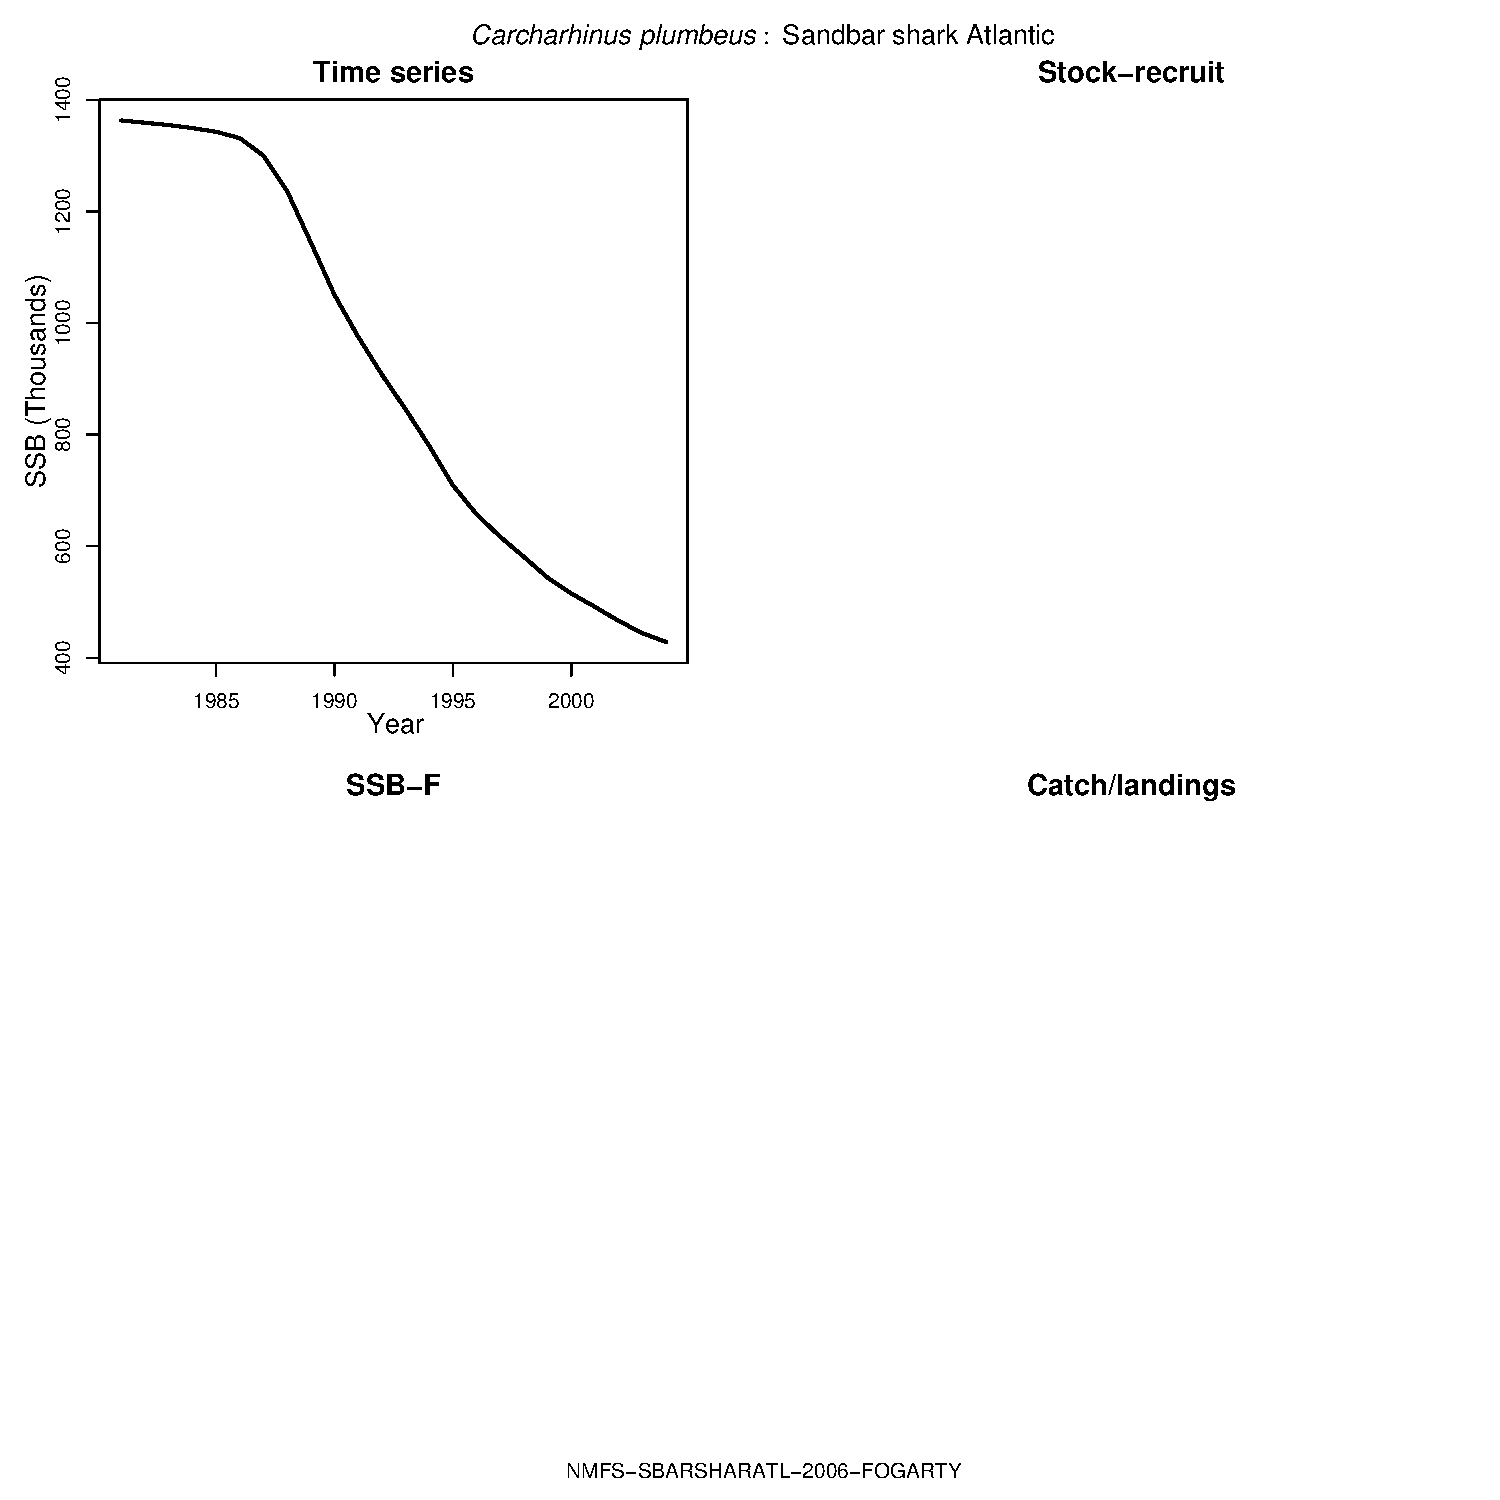
\includegraphics[width=1.2\textwidth]{../R/figures/NMFS-SBARSHARATL-2006-FOGARTY.pdf}
\end{center}

\subsubsection{Rhizoprionodon terraenovae - Atlantic sharpnose shark}\index{Atlantic sharpnose shark}\index{Rhizoprionodon terraenovae}\index{Carcharhinidae!Rhizoprionodon terraenovae}
\begin{center}
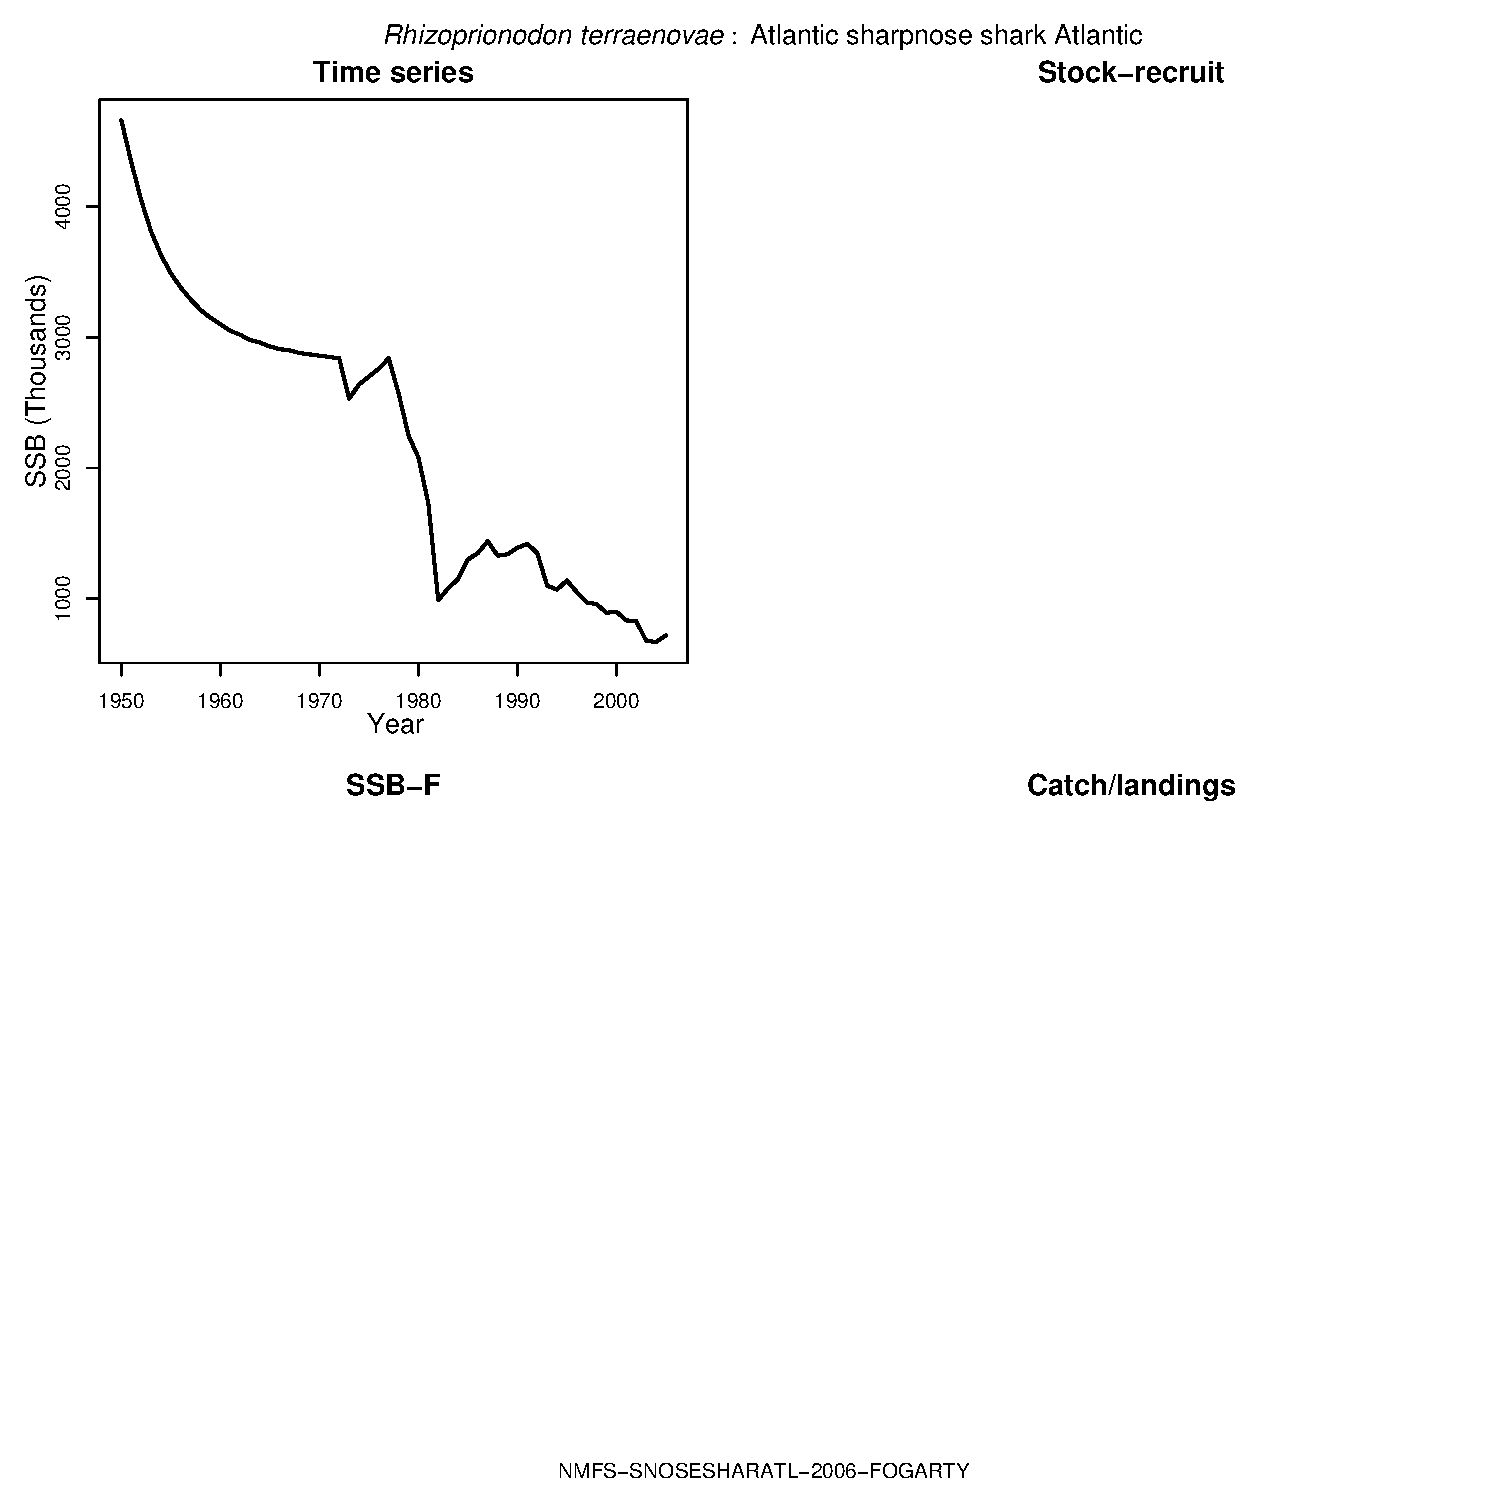
\includegraphics[width=1.2\textwidth]{../R/figures/NMFS-SNOSESHARATL-2006-FOGARTY.pdf}
\end{center}

\subsection{Sphyrnidae}\index{Sphyrnidae}\index{Carcharhiniformes!Sphyrnidae}

\subsubsection{Sphyrna tiburo - Bonnethead shark}\index{Bonnethead shark}\index{Sphyrna tiburo}\index{Sphyrnidae!Sphyrna tiburo}
\begin{center}
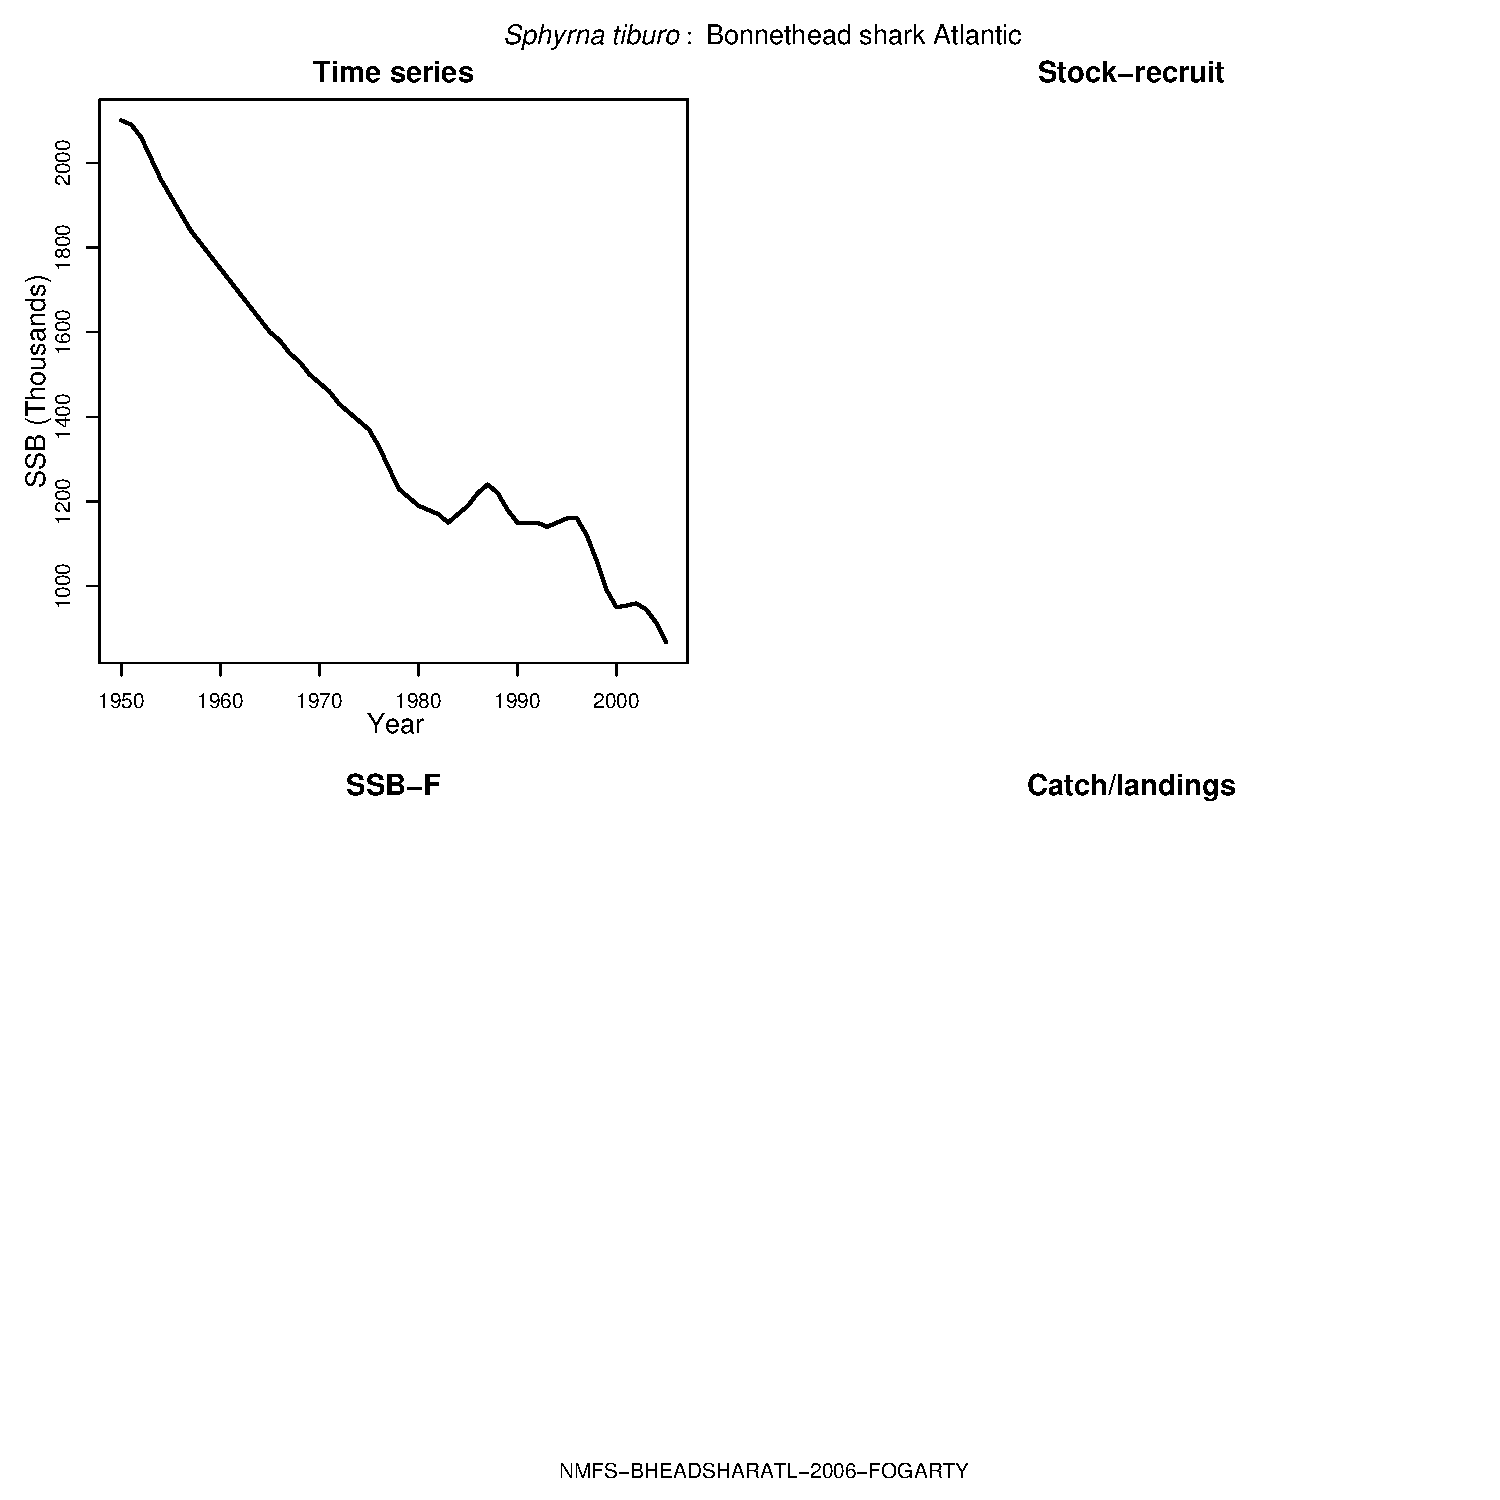
\includegraphics[width=1.2\textwidth]{../R/figures/NMFS-BHEADSHARATL-2006-FOGARTY.pdf}
\end{center}

\section{Clupeiformes}\index{Clupeiformes}

\subsection{Clupeidae}\index{Clupeidae}\index{Clupeiformes!Clupeidae}

\subsubsection{Clupea harengus - Herring}\index{Herring}\index{Clupea harengus}\index{Clupeidae!Clupea harengus}
\begin{center}
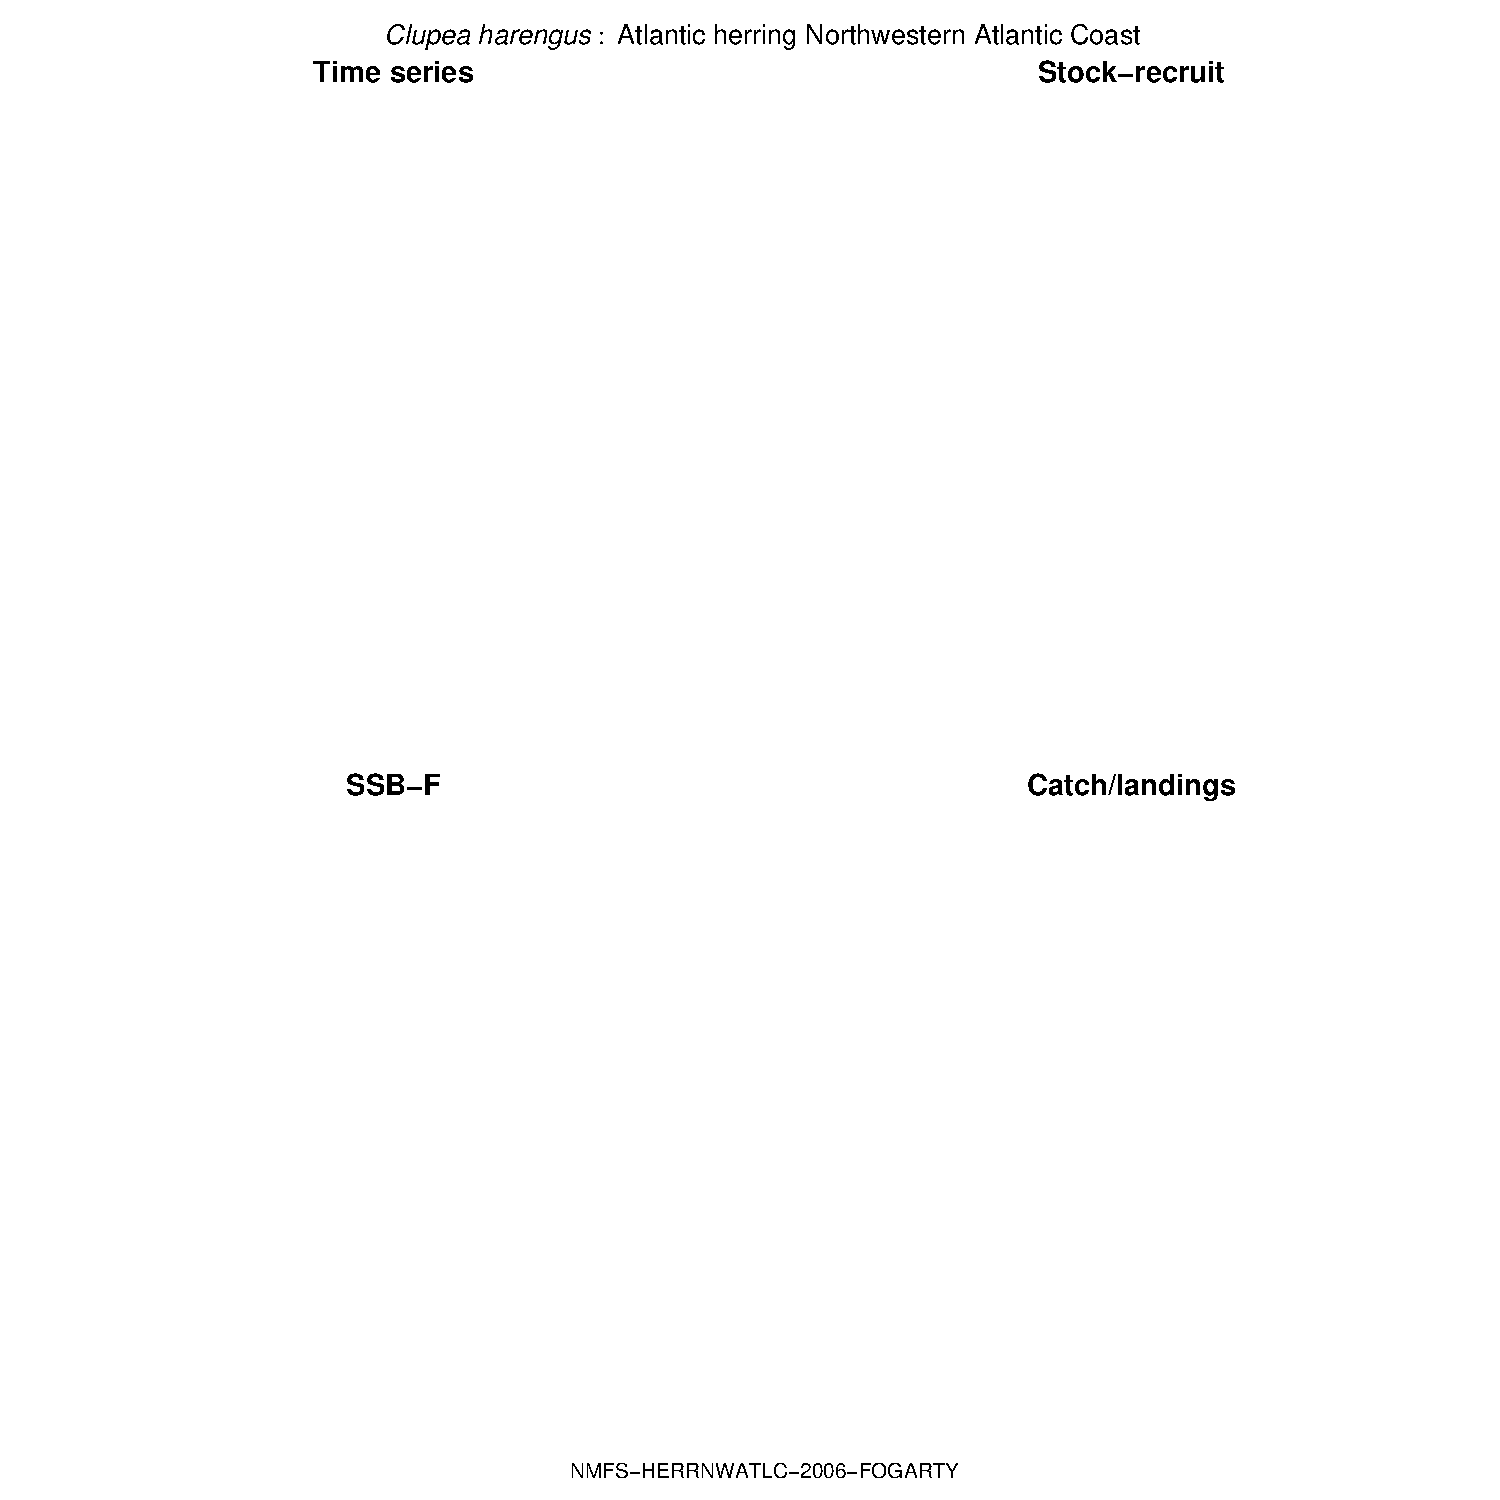
\includegraphics[width=1.2\textwidth]{../R/figures/NMFS-HERRNWATLC-2006-FOGARTY.pdf}
\end{center}

\subsubsection{Clupea harengus - Herring}\index{Herring}\index{Clupea harengus}\index{Clupeidae!Clupea harengus}
\begin{center}
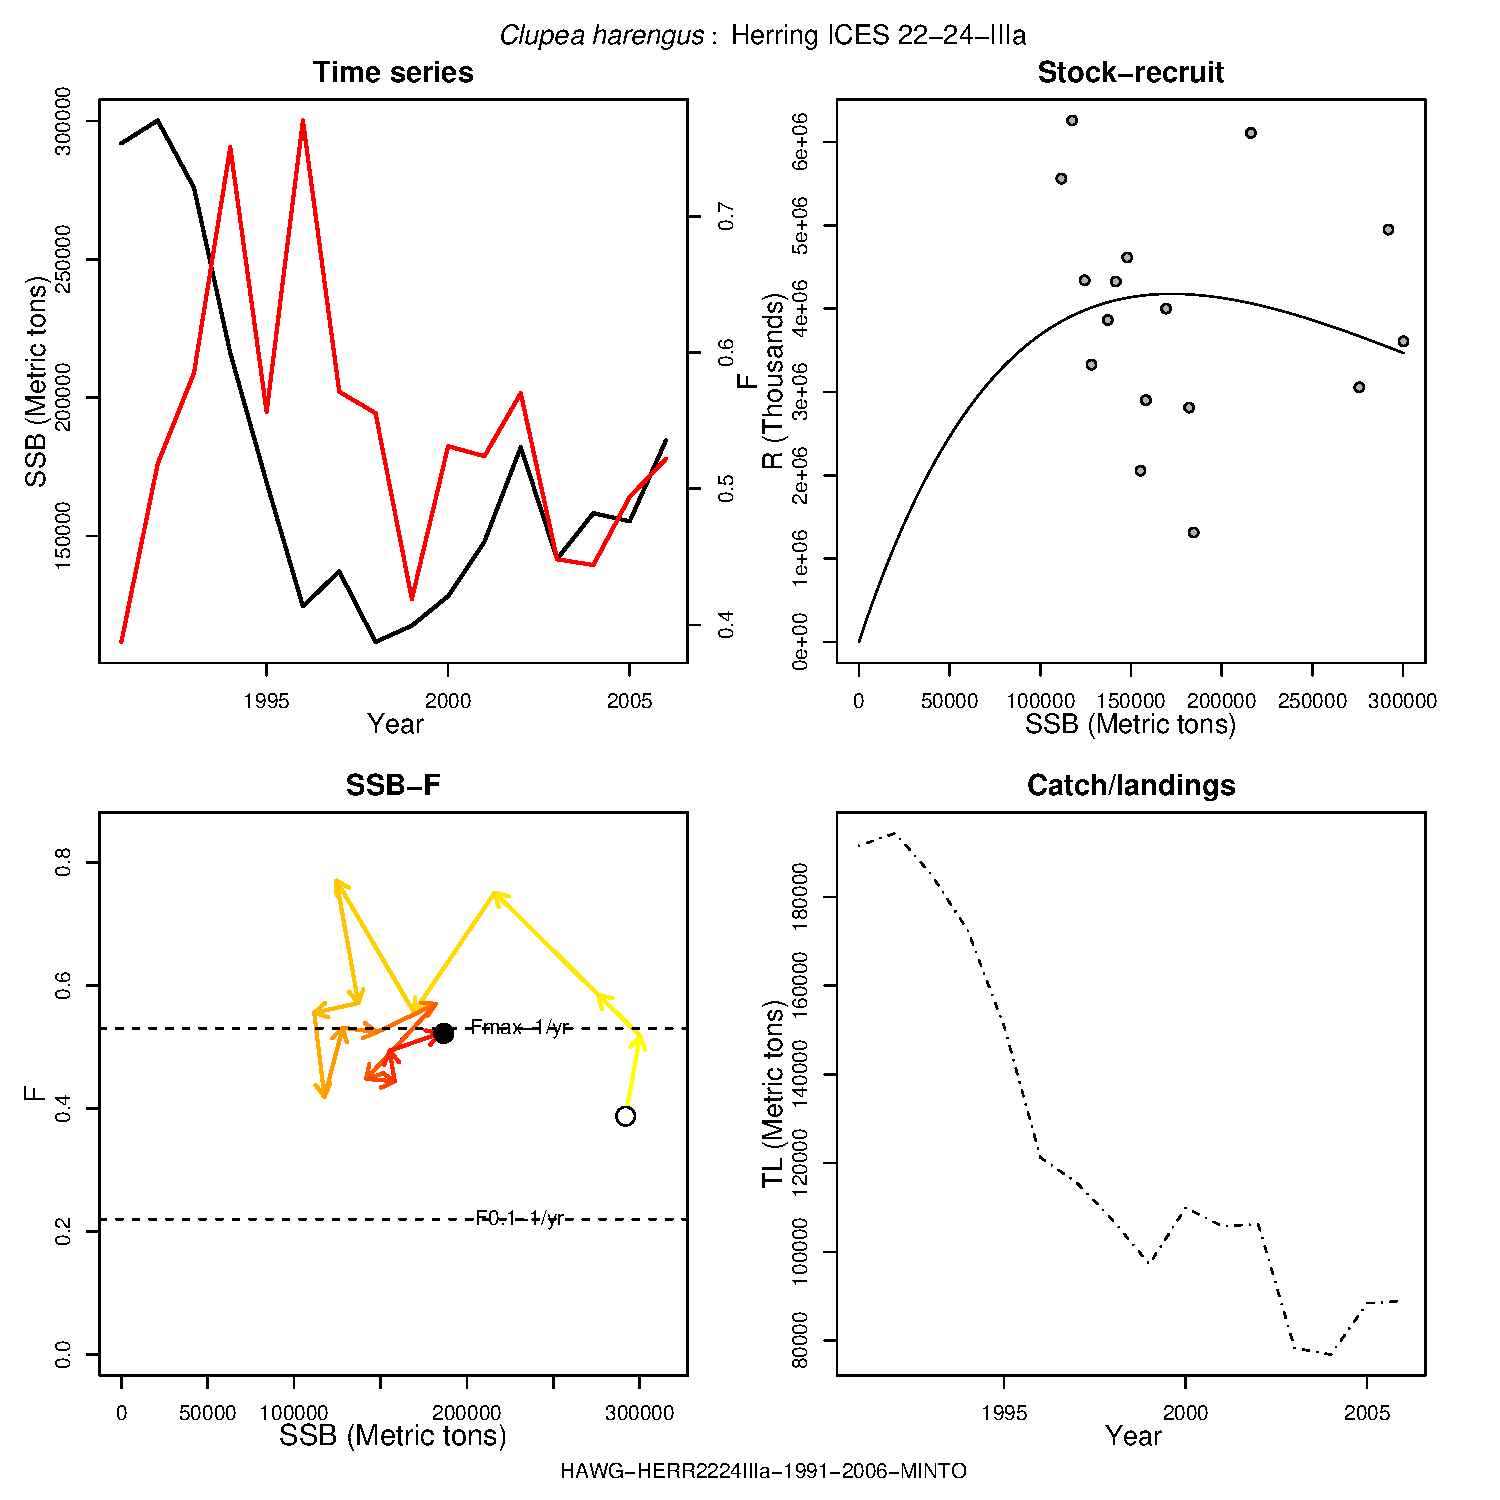
\includegraphics[width=1.2\textwidth]{../R/figures/HAWG-HERR2224IIIa-1991-2006-MINTO.pdf}
\end{center}

\subsubsection{Clupea harengus - Herring}\index{Herring}\index{Clupea harengus}\index{Clupeidae!Clupea harengus}
\begin{center}
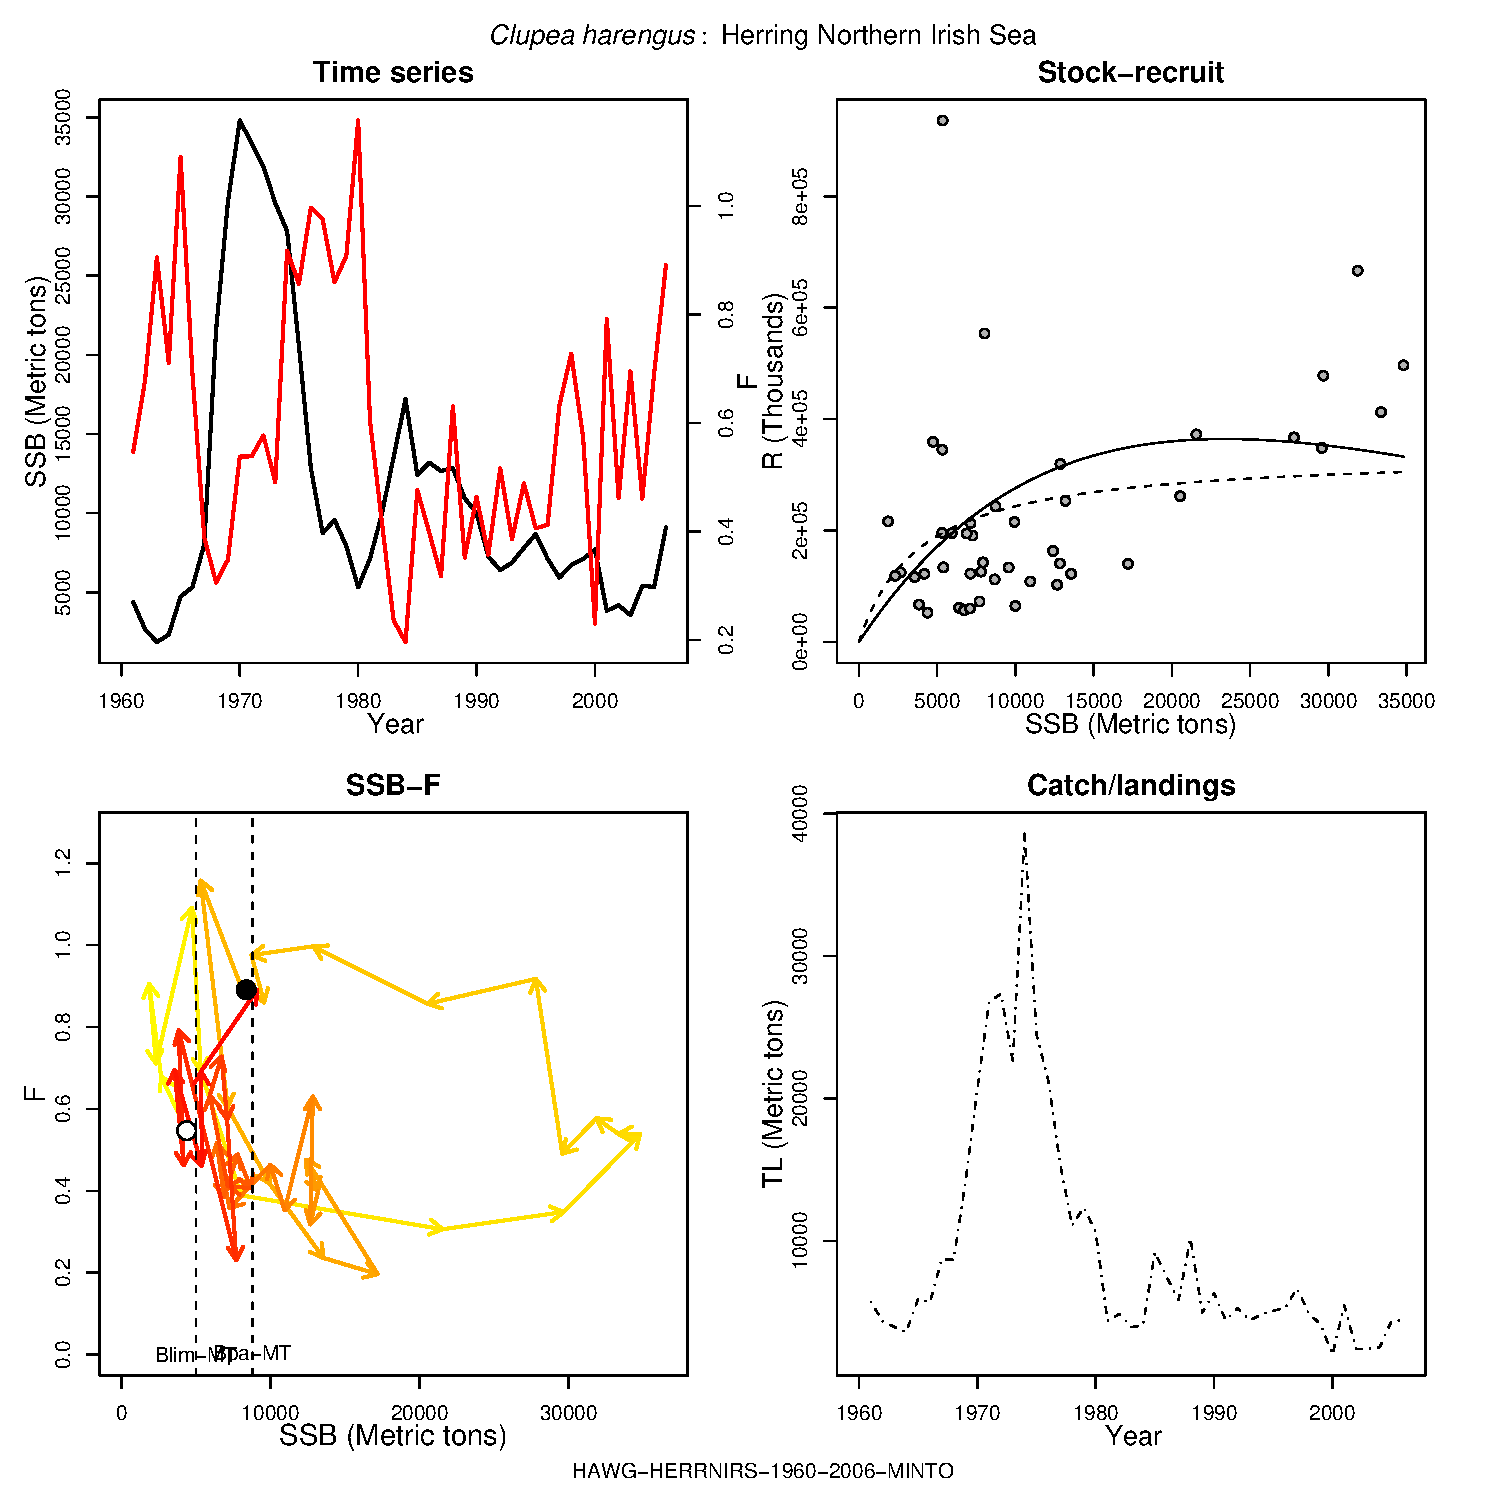
\includegraphics[width=1.2\textwidth]{../R/figures/HAWG-HERRNIRS-1960-2006-MINTO.pdf}
\end{center}

\subsubsection{Clupea harengus - Herring}\index{Herring}\index{Clupea harengus}\index{Clupeidae!Clupea harengus}
\begin{center}
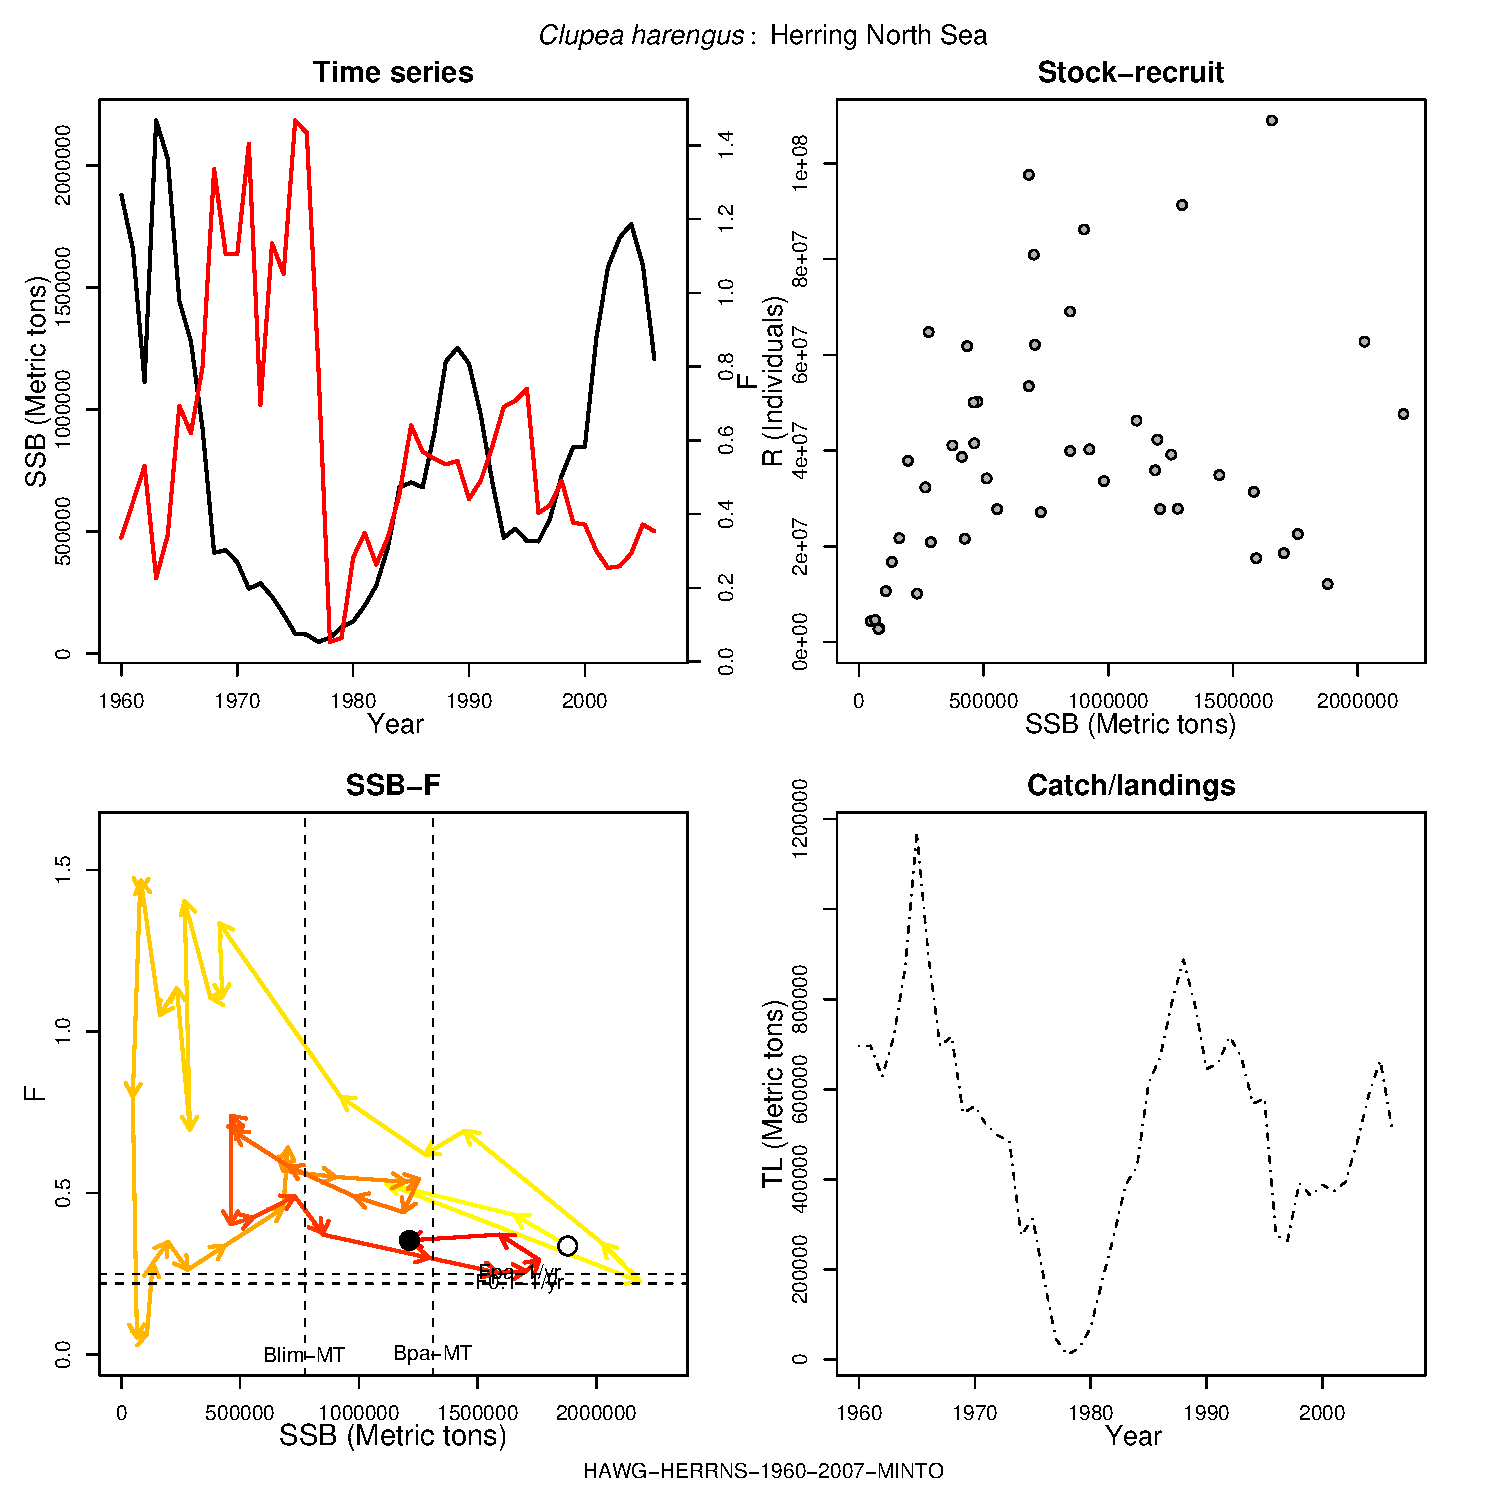
\includegraphics[width=1.2\textwidth]{../R/figures/HAWG-HERRNS-1960-2007-MINTO.pdf}
\end{center}

\subsubsection{Clupea harengus - Herring}\index{Herring}\index{Clupea harengus}\index{Clupeidae!Clupea harengus}
\begin{center}
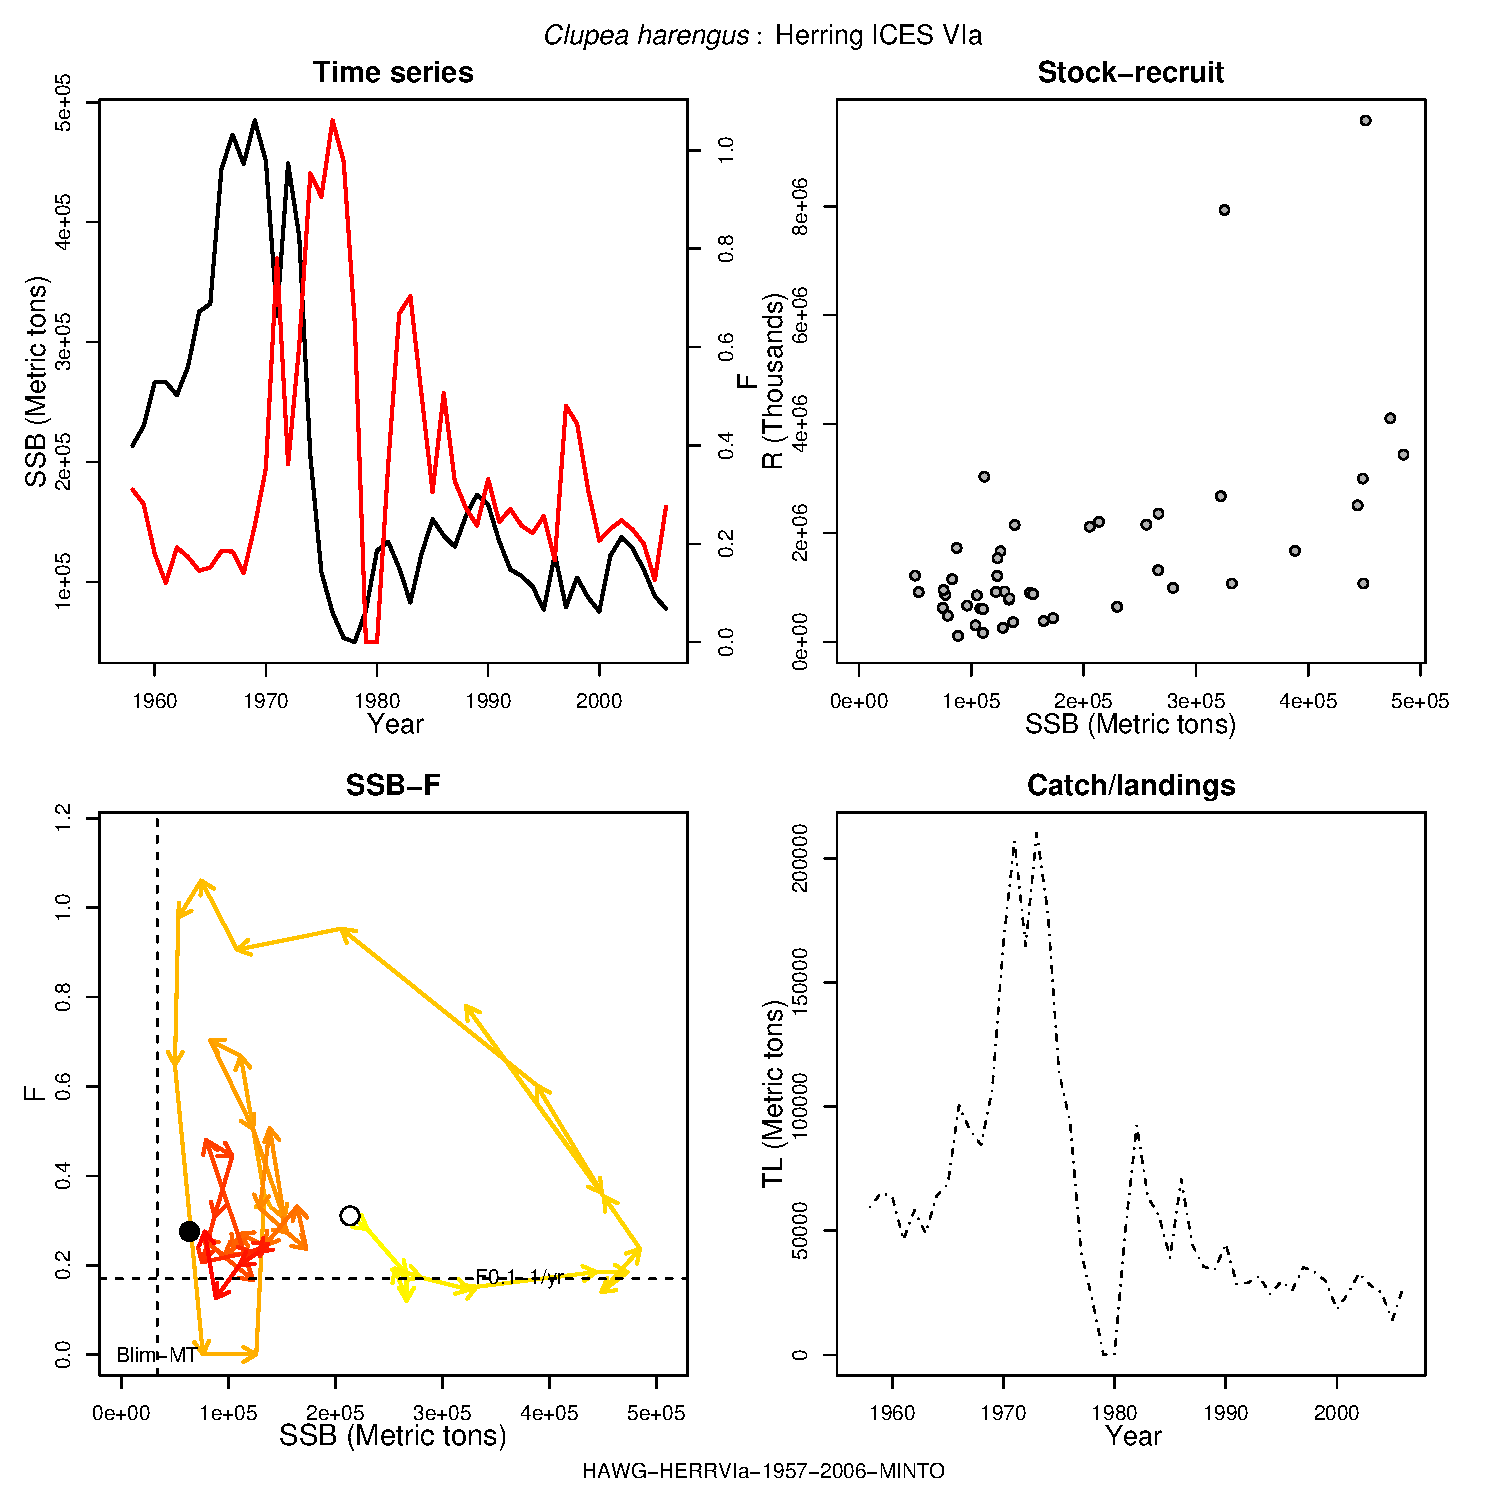
\includegraphics[width=1.2\textwidth]{../R/figures/HAWG-HERRVIa-1957-2006-MINTO.pdf}
\end{center}

\subsubsection{Clupea harengus - Herring}\index{Herring}\index{Clupea harengus}\index{Clupeidae!Clupea harengus}
\begin{center}
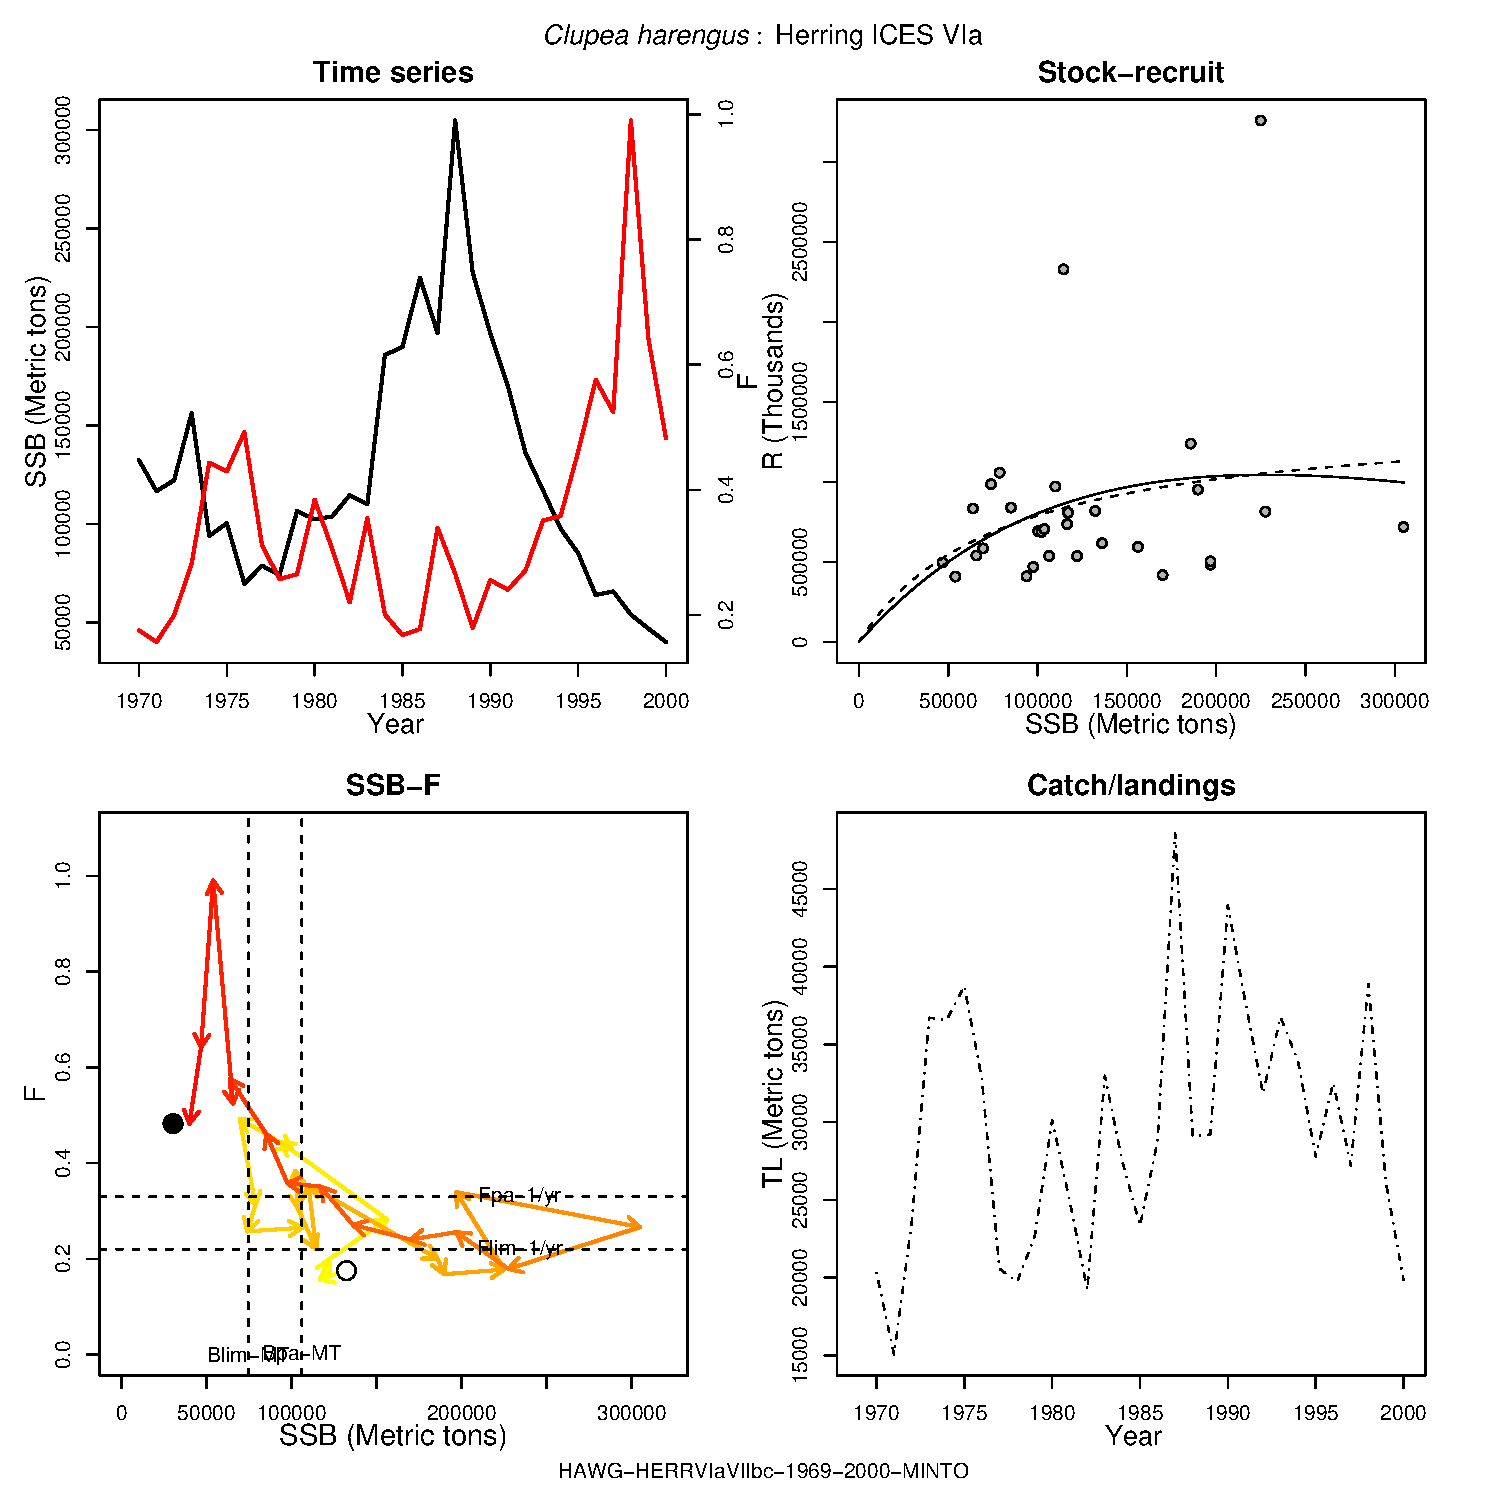
\includegraphics[width=1.2\textwidth]{../R/figures/HAWG-HERRVIaVIIbc-1969-2000-MINTO.pdf}
\end{center}

\subsubsection{Clupea harengus - Herring}\index{Herring}\index{Clupea harengus}\index{Clupeidae!Clupea harengus}
\begin{center}
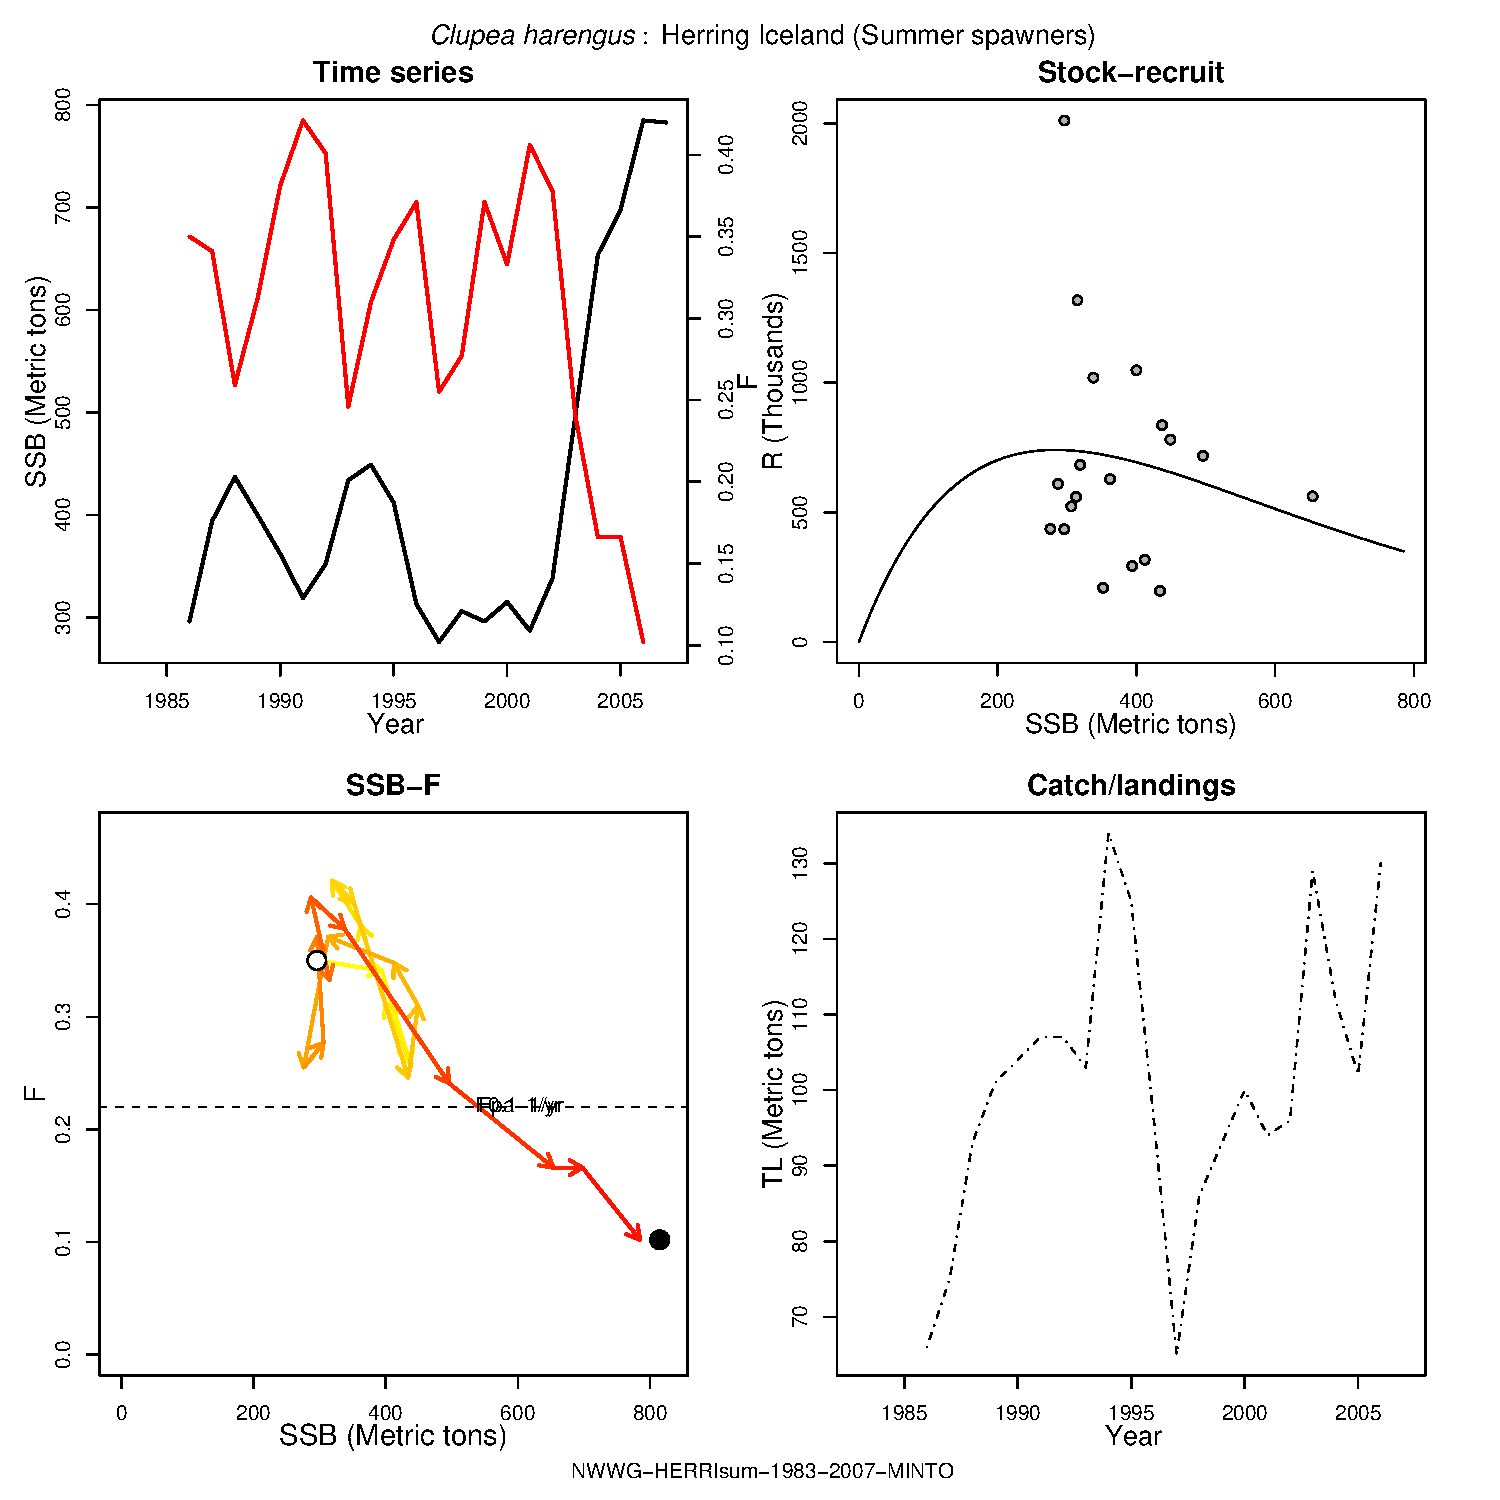
\includegraphics[width=1.2\textwidth]{../R/figures/NWWG-HERRIsum-1983-2007-MINTO.pdf}
\end{center}

\subsubsection{Clupea harengus - Herring}\index{Herring}\index{Clupea harengus}\index{Clupeidae!Clupea harengus}
\begin{center}
\includegraphics[width=1.2\textwidth]{../R/figures/PHONYassessorid-HERRIsum-1946-2000-MYERS.pdf}
\end{center}

\subsubsection{Clupea harengus - Herring}\index{Herring}\index{Clupea harengus}\index{Clupeidae!Clupea harengus}
\begin{center}
\includegraphics[width=1.2\textwidth]{../R/figures/PHONYassessorid-HERRNIRS-1971-2000-MYERS.pdf}
\end{center}

\subsubsection{Clupea harengus - Herring}\index{Herring}\index{Clupea harengus}\index{Clupeidae!Clupea harengus}
\begin{center}
\includegraphics[width=1.2\textwidth]{../R/figures/PHONYassessorid-HERRNS-1903-1990-MYERS.pdf}
\end{center}

\subsubsection{Clupea harengus - Herring}\index{Herring}\index{Clupea harengus}\index{Clupeidae!Clupea harengus}
\begin{center}
\includegraphics[width=1.2\textwidth]{../R/figures/PHONYassessorid-HERRVIaVIIbc-1969-2000-MYERS.pdf}
\end{center}

\subsubsection{Clupea harengus - Herring}\index{Herring}\index{Clupea harengus}\index{Clupeidae!Clupea harengus}
\begin{center}
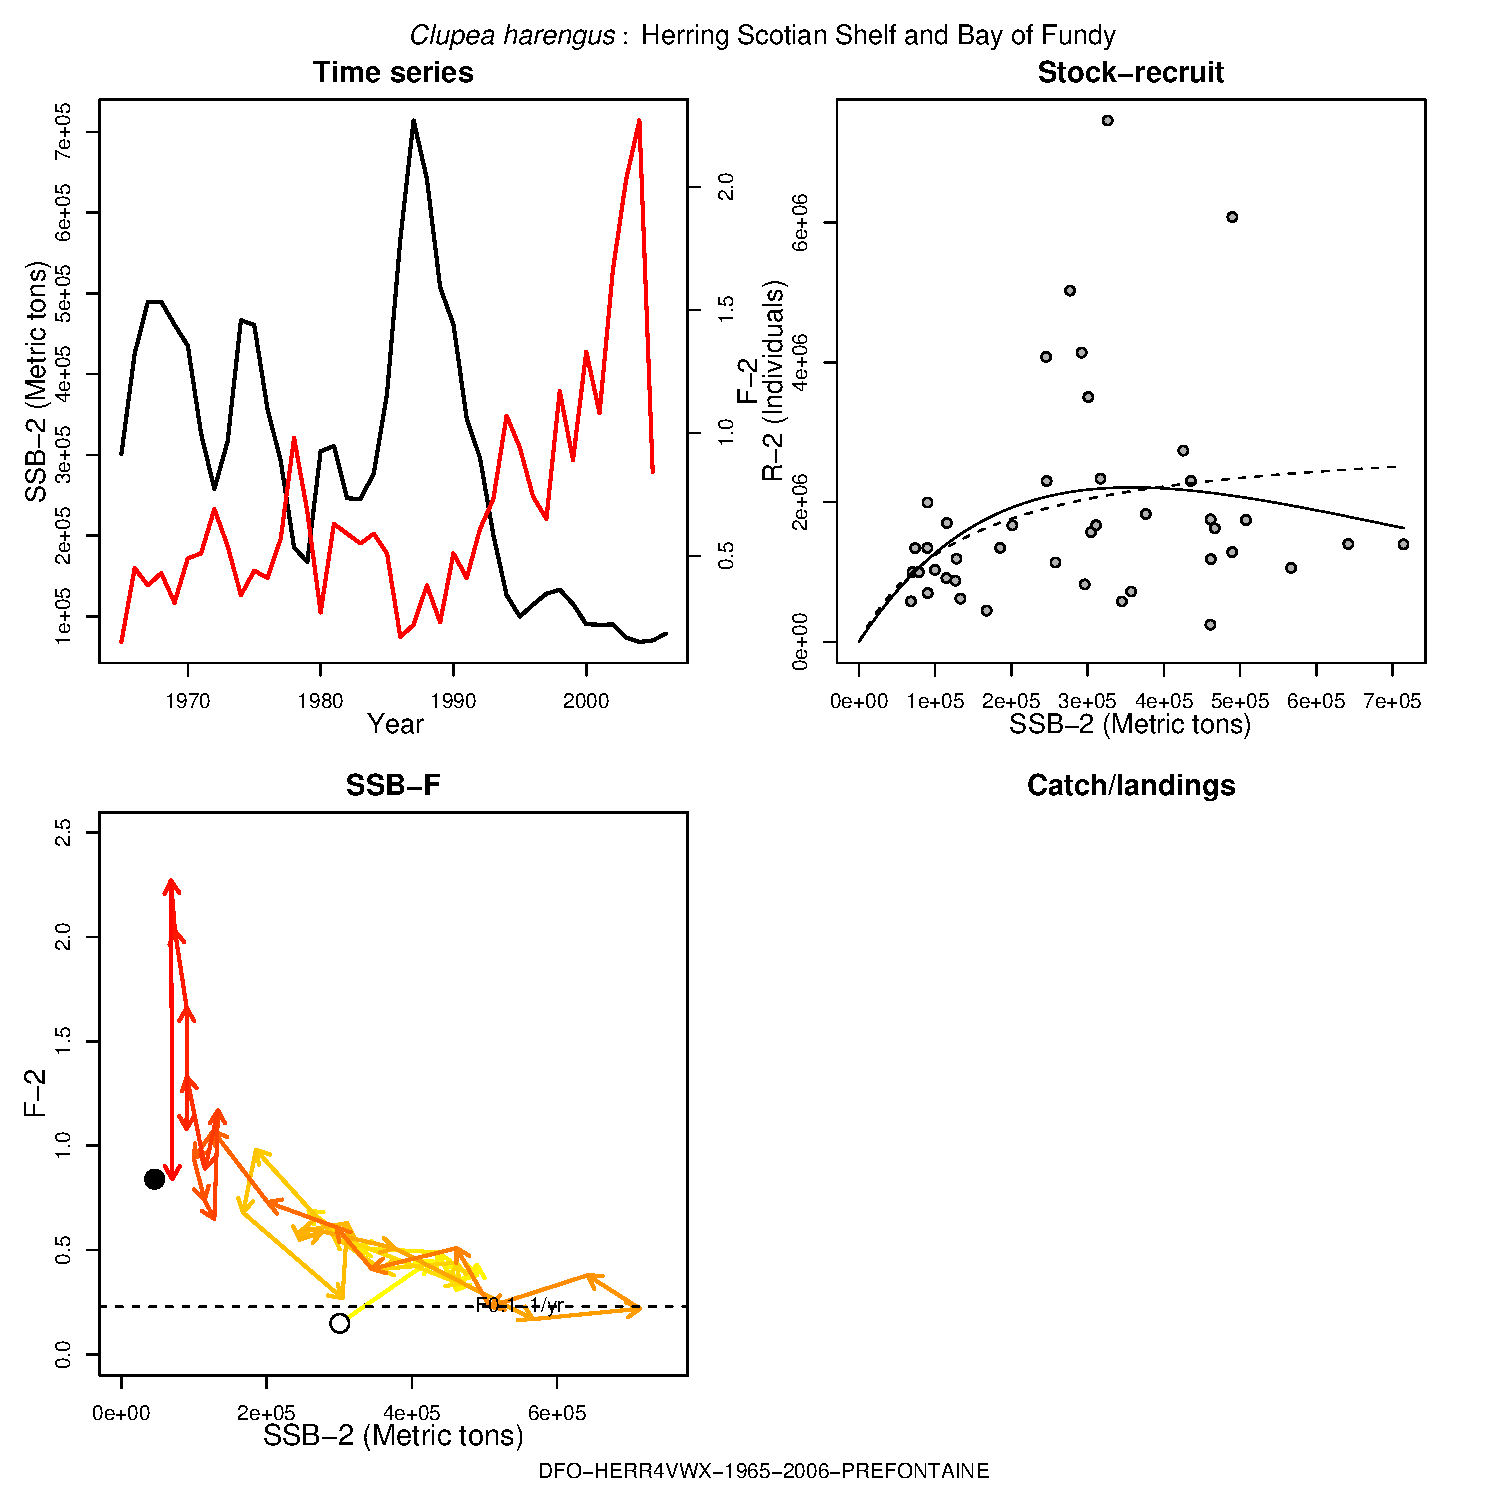
\includegraphics[width=1.2\textwidth]{../R/figures/DFO-HERR4VWX-1965-2006-PREFONTAINE.pdf}
\end{center}

\subsubsection{Clupea harengus - Herring}\index{Herring}\index{Clupea harengus}\index{Clupeidae!Clupea harengus}
\begin{center}
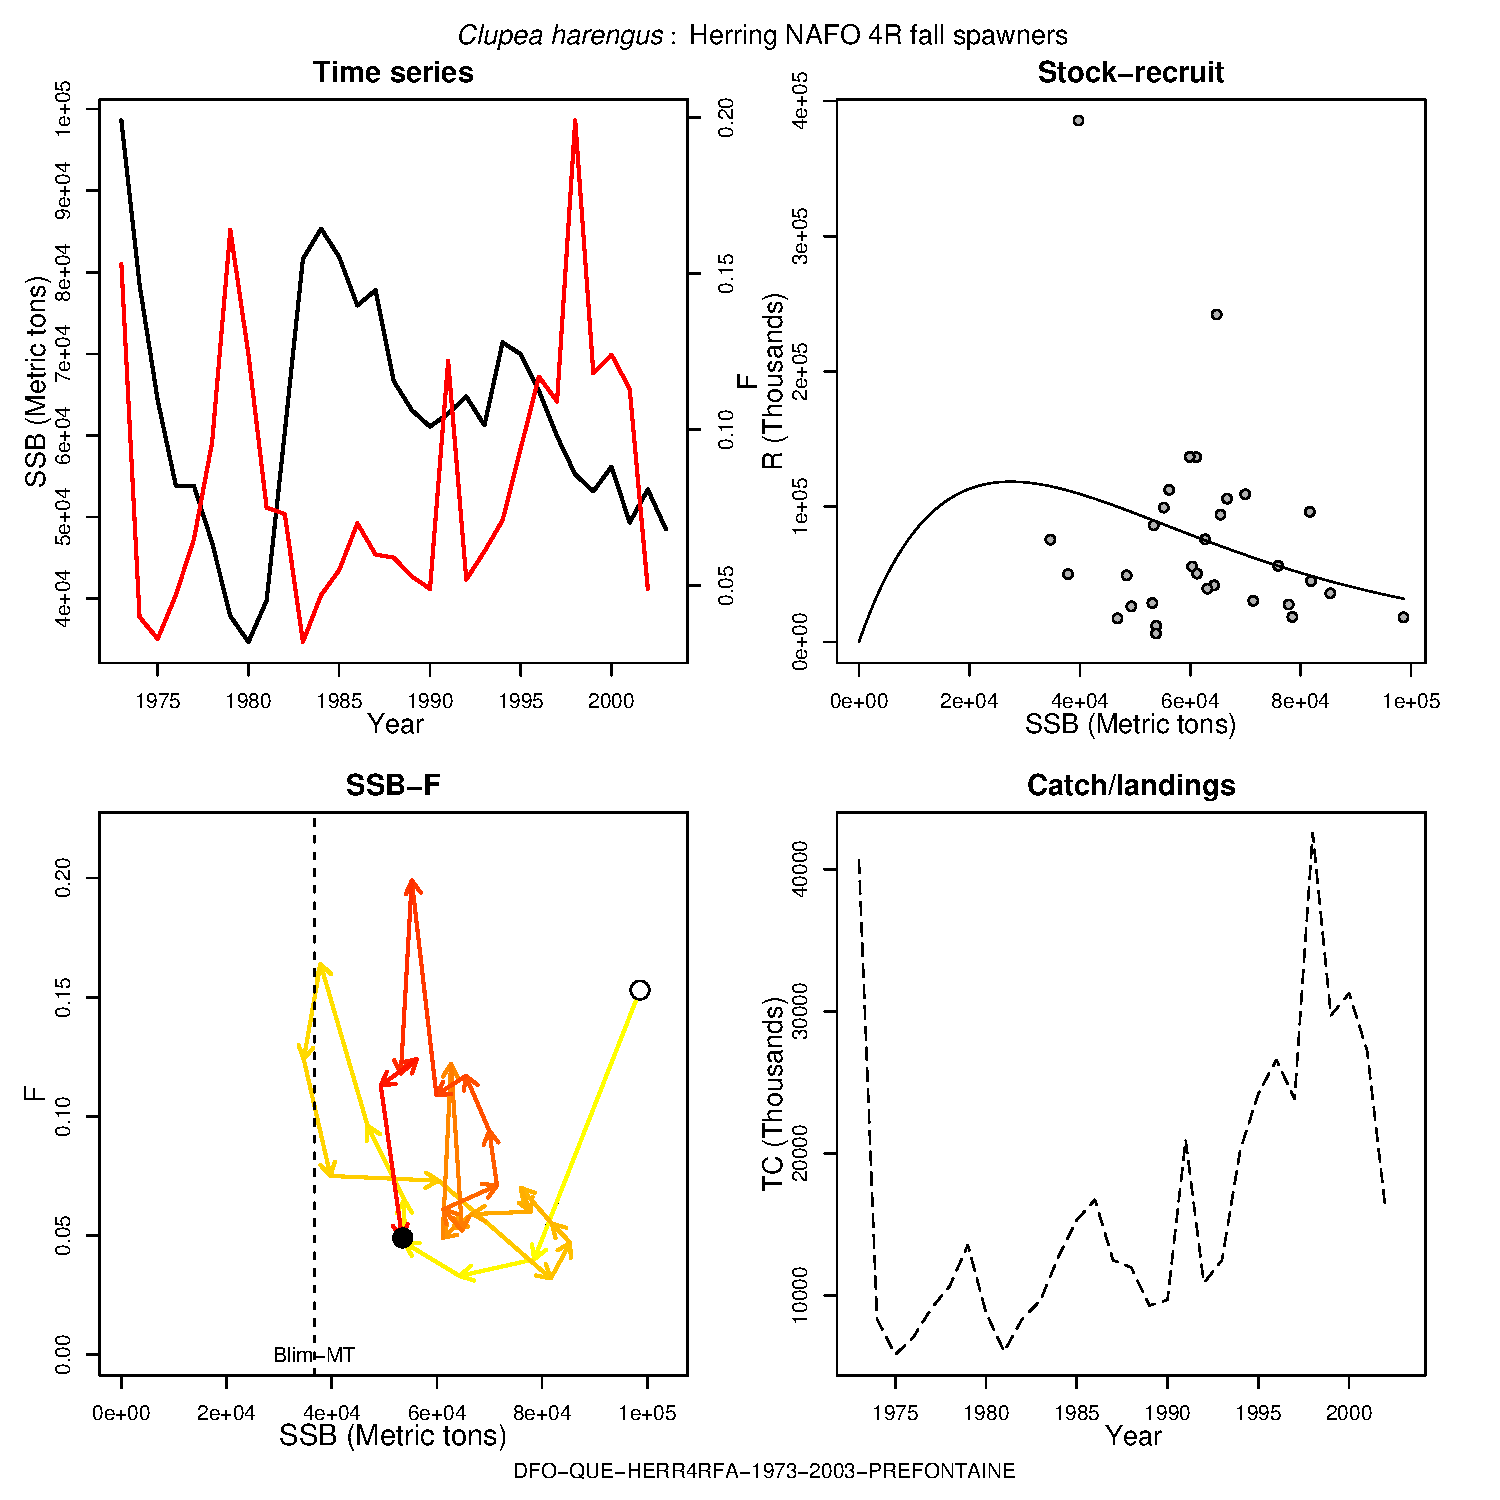
\includegraphics[width=1.2\textwidth]{../R/figures/DFO-QUE-HERR4RFA-1973-2003-PREFONTAINE.pdf}
\end{center}

\subsubsection{Clupea harengus - Herring}\index{Herring}\index{Clupea harengus}\index{Clupeidae!Clupea harengus}
\begin{center}
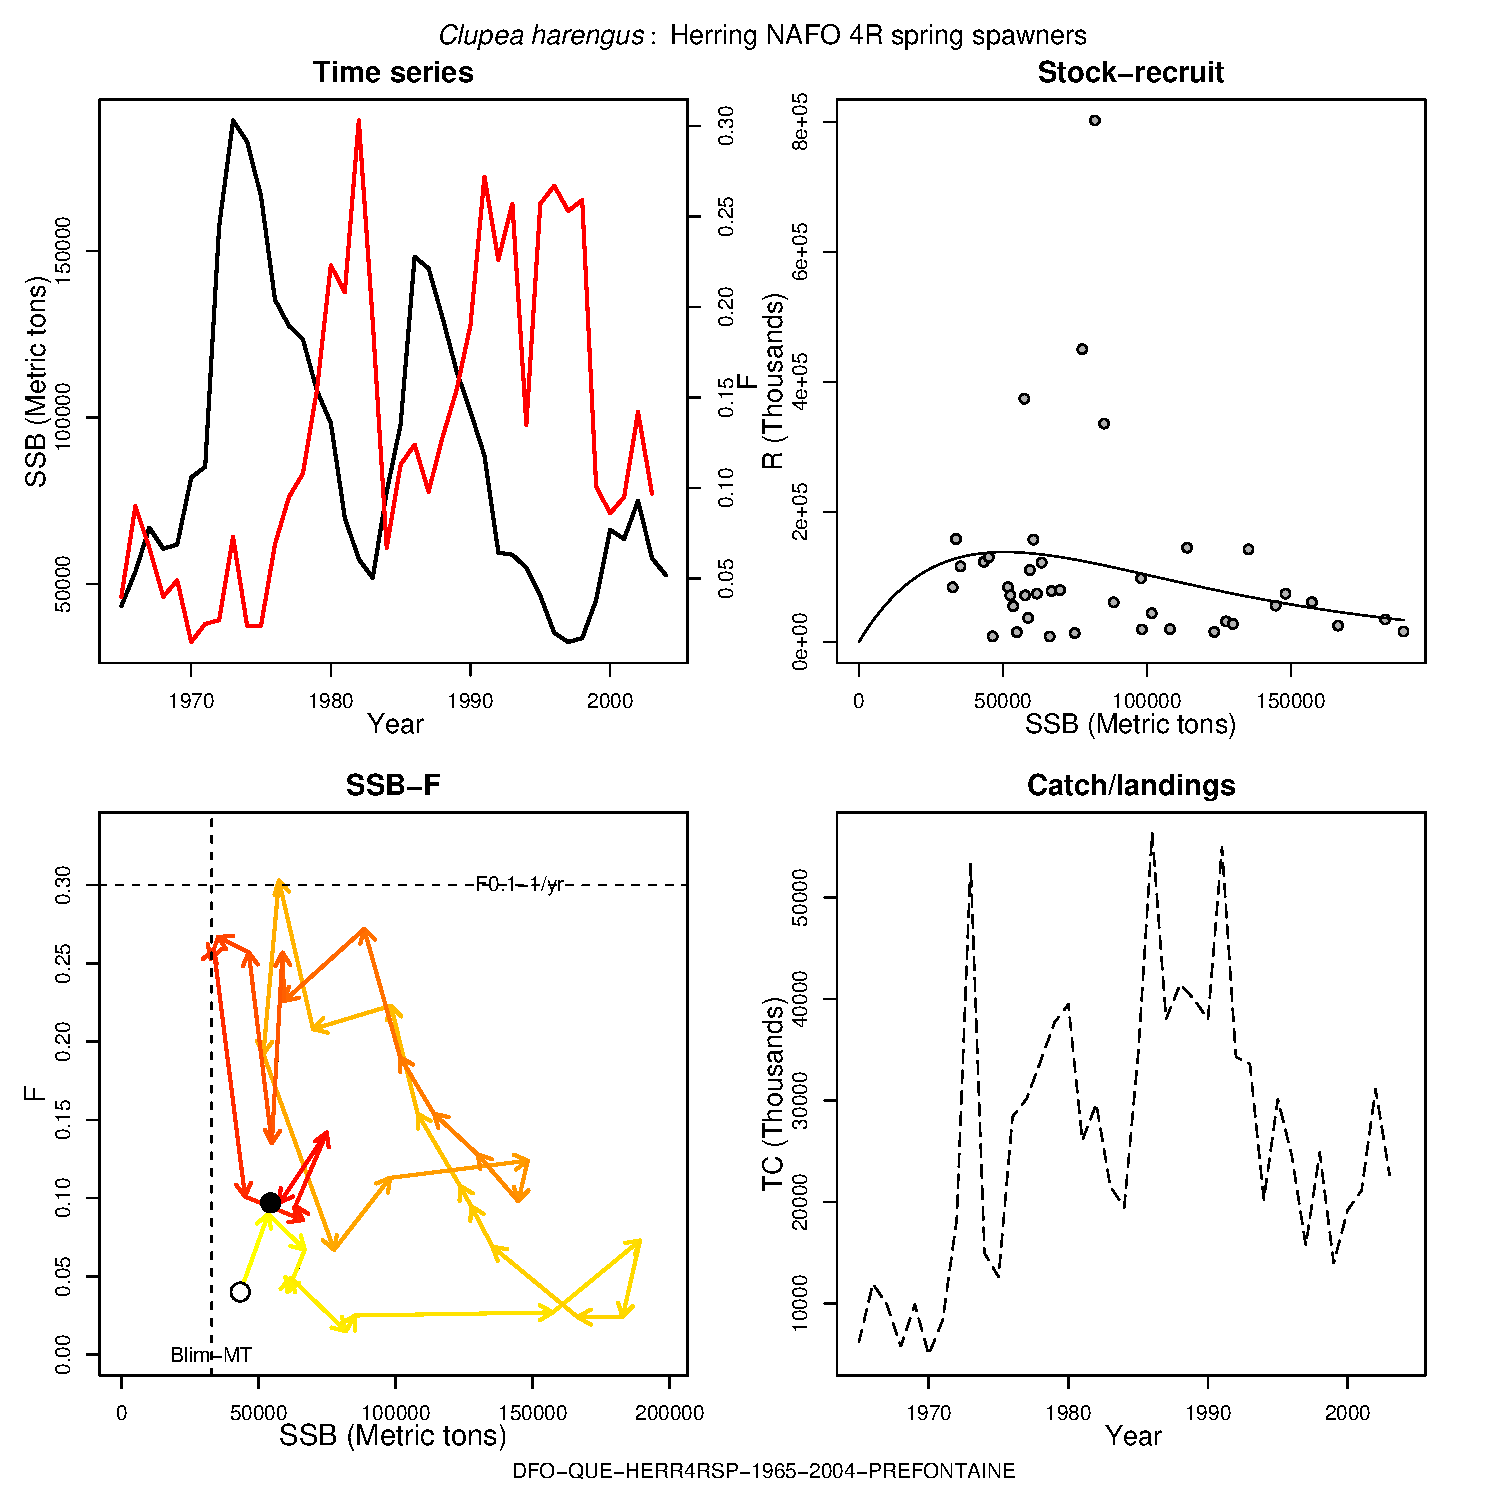
\includegraphics[width=1.2\textwidth]{../R/figures/DFO-QUE-HERR4RSP-1965-2004-PREFONTAINE.pdf}
\end{center}

\subsubsection{Clupea pallasii - Pacific herring}\index{Pacific herring}\index{Clupea pallasii}\index{Clupeidae!Clupea pallasii}
\begin{center}
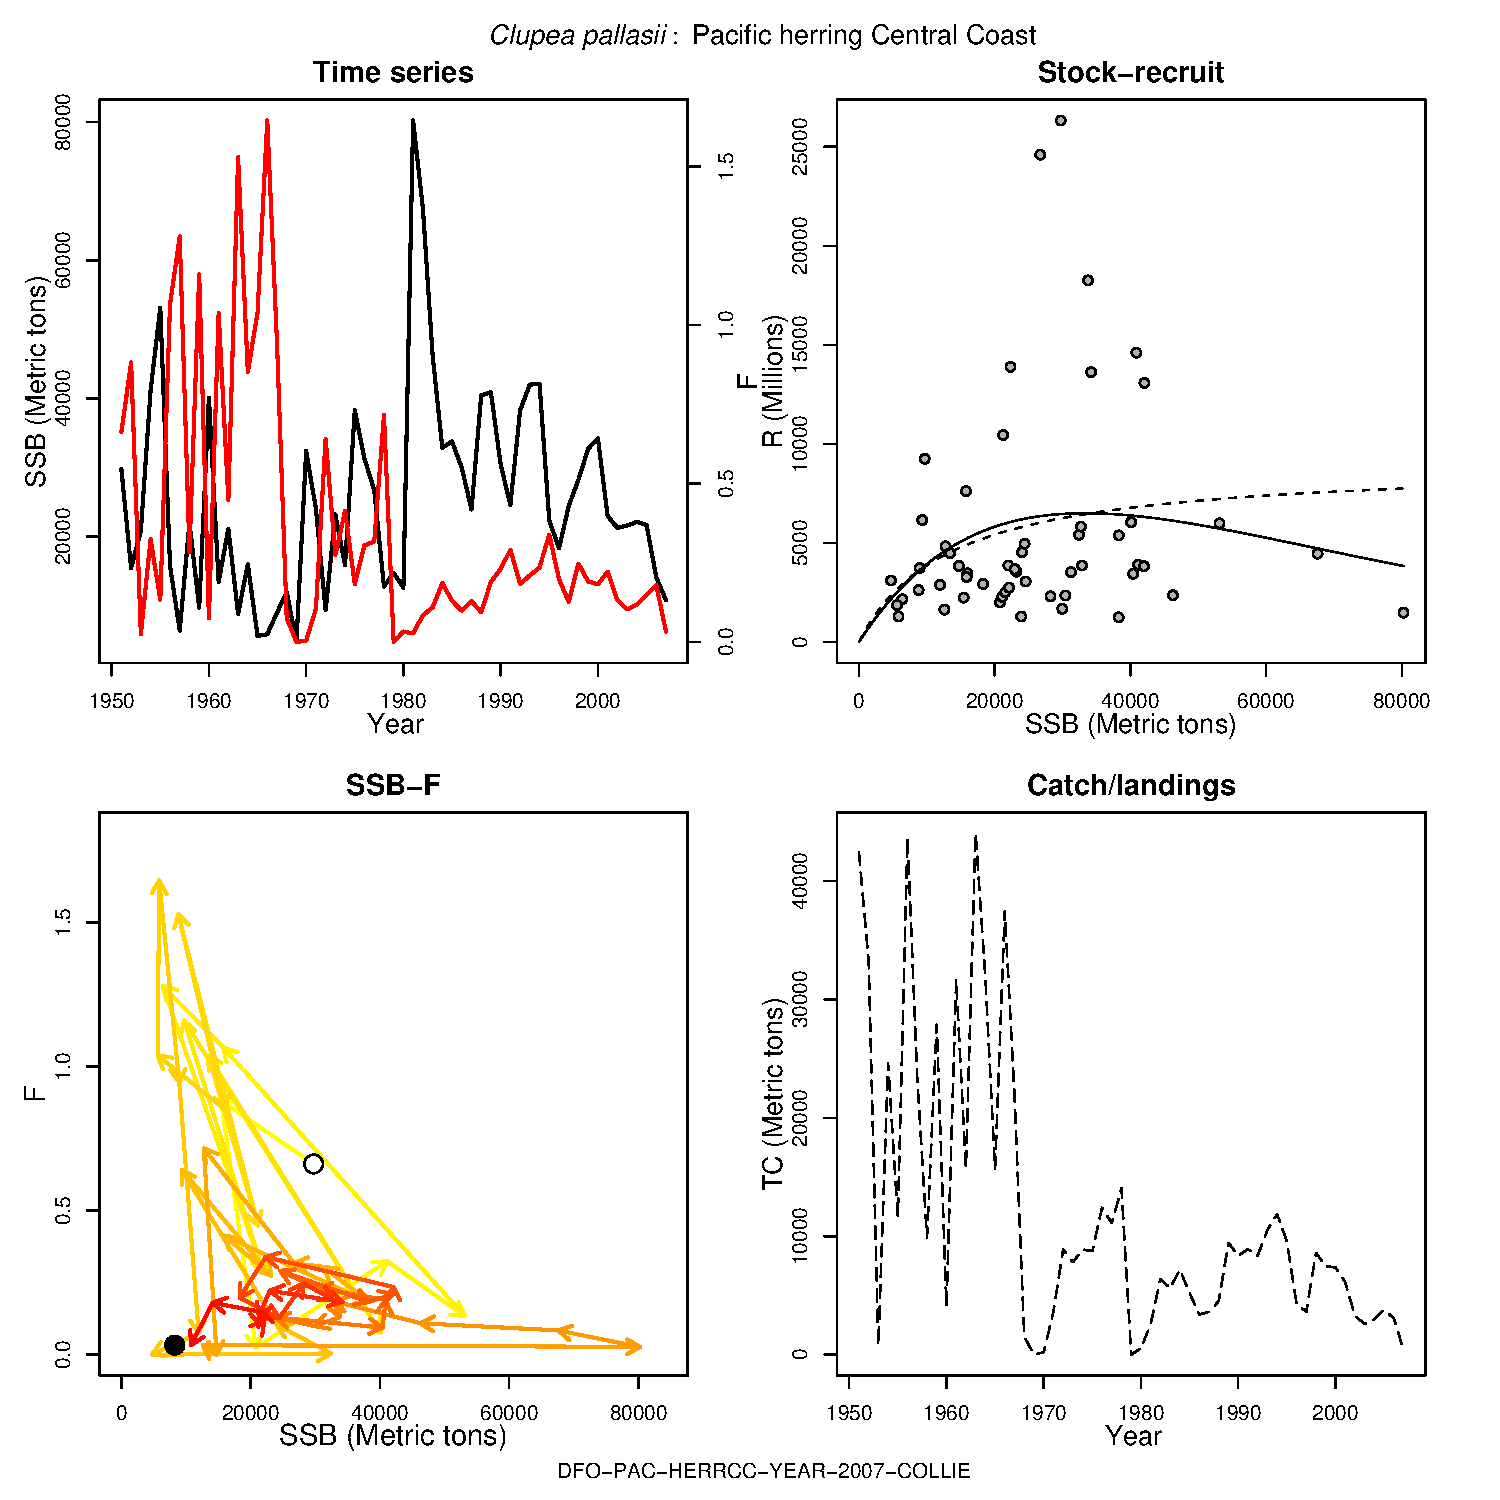
\includegraphics[width=1.2\textwidth]{../R/figures/DFO-PAC-HERRCC-YEAR-2007-COLLIE.pdf}
\end{center}

\subsubsection{Clupea pallasii - Pacific herring}\index{Pacific herring}\index{Clupea pallasii}\index{Clupeidae!Clupea pallasii}
\begin{center}
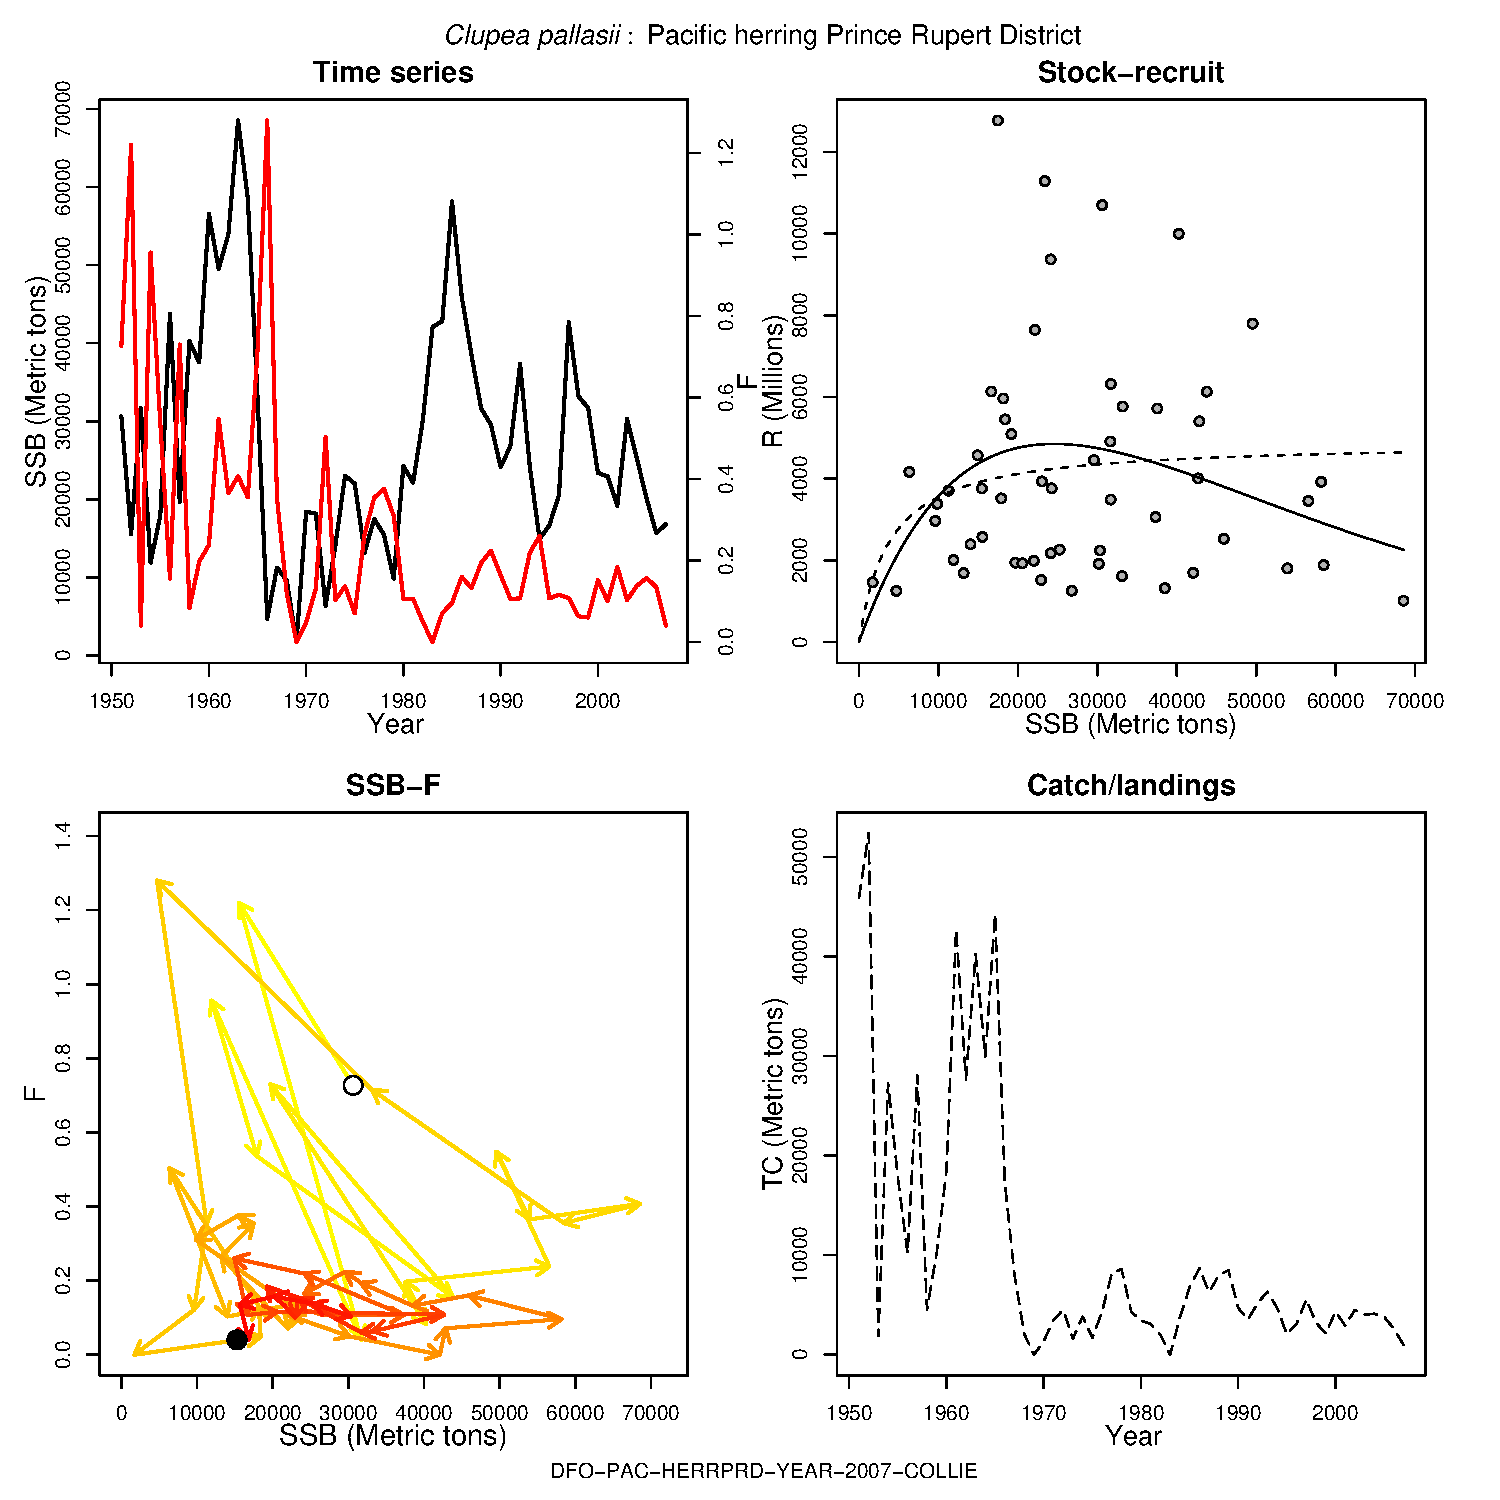
\includegraphics[width=1.2\textwidth]{../R/figures/DFO-PAC-HERRPRD-YEAR-2007-COLLIE.pdf}
\end{center}

\subsubsection{Clupea pallasii - Pacific herring}\index{Pacific herring}\index{Clupea pallasii}\index{Clupeidae!Clupea pallasii}
\begin{center}
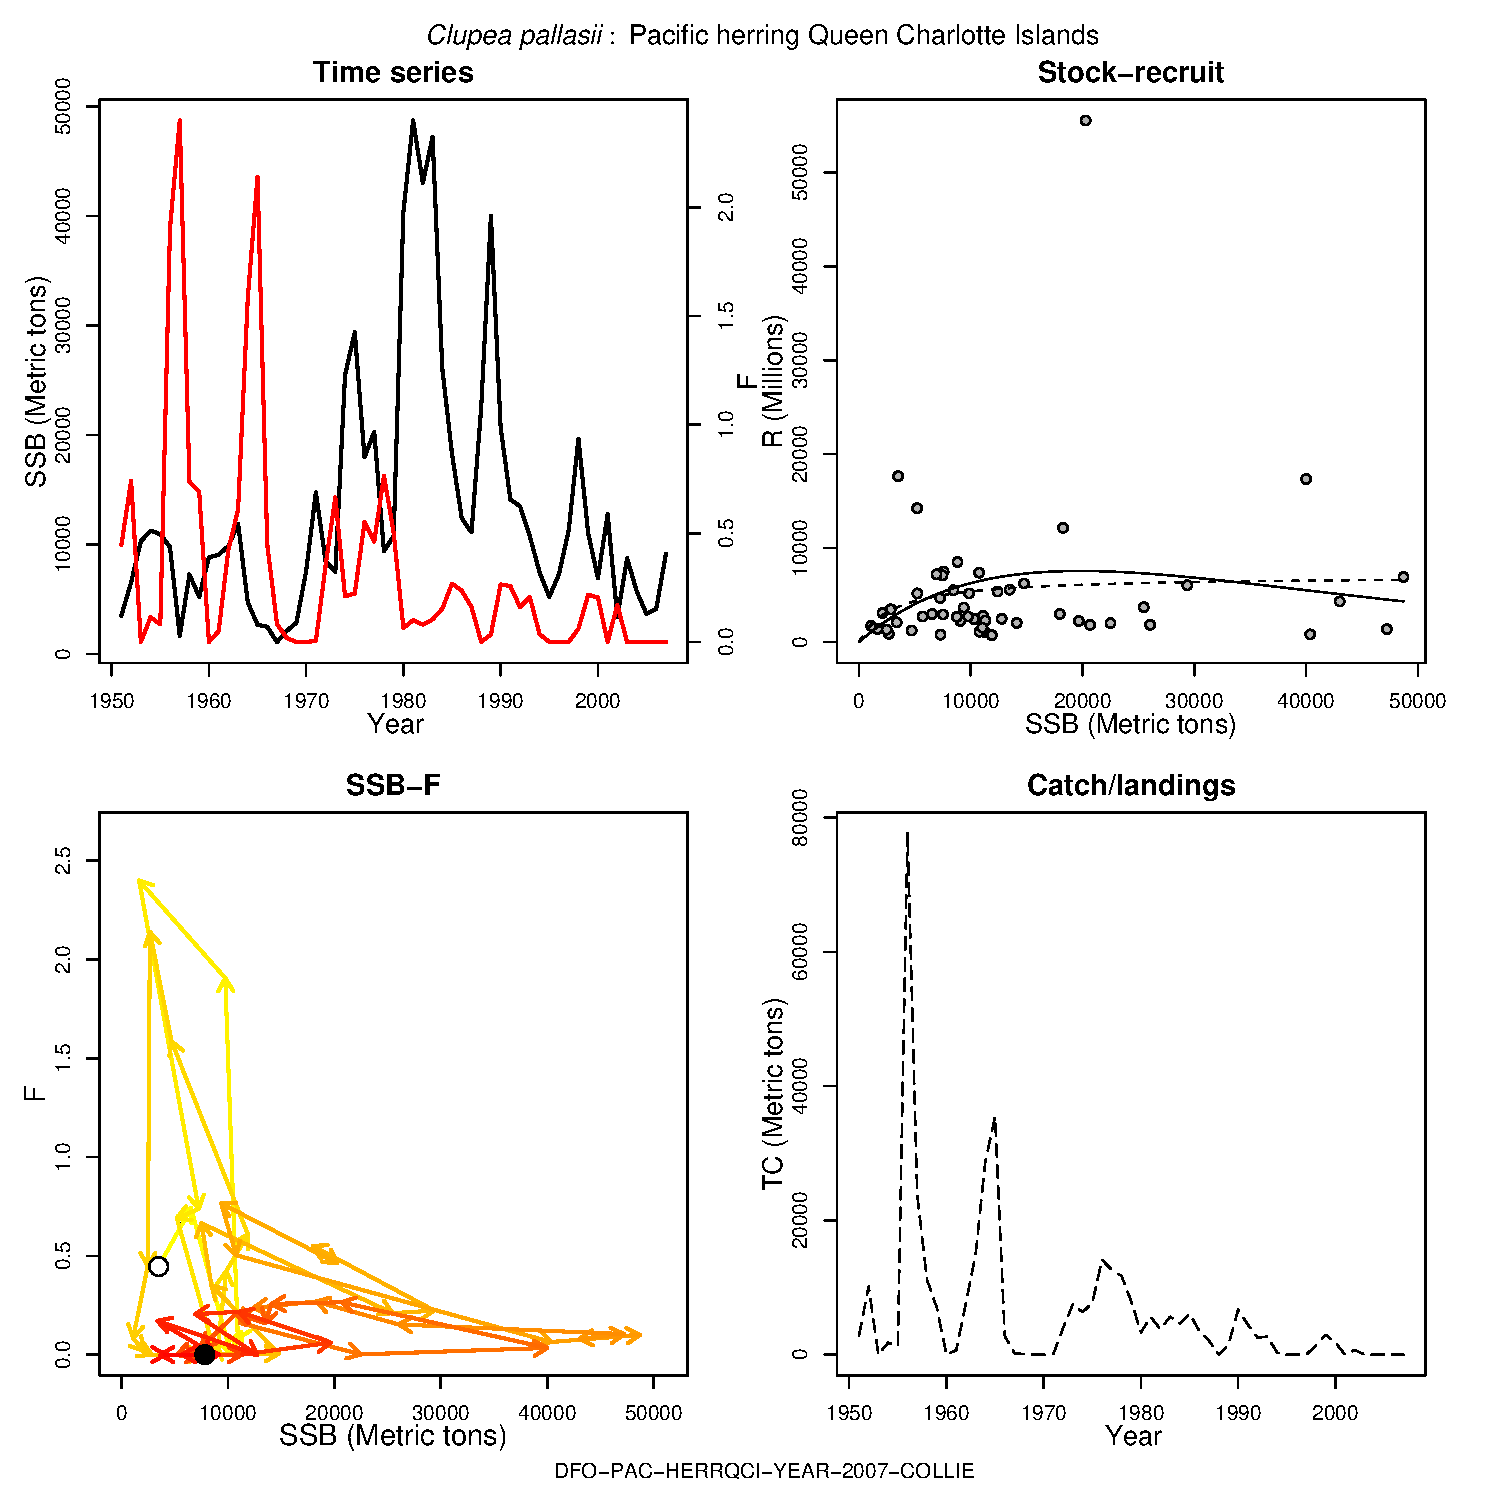
\includegraphics[width=1.2\textwidth]{../R/figures/DFO-PAC-HERRQCI-YEAR-2007-COLLIE.pdf}
\end{center}

\subsubsection{Clupea pallasii - Pacific herring}\index{Pacific herring}\index{Clupea pallasii}\index{Clupeidae!Clupea pallasii}
\begin{center}
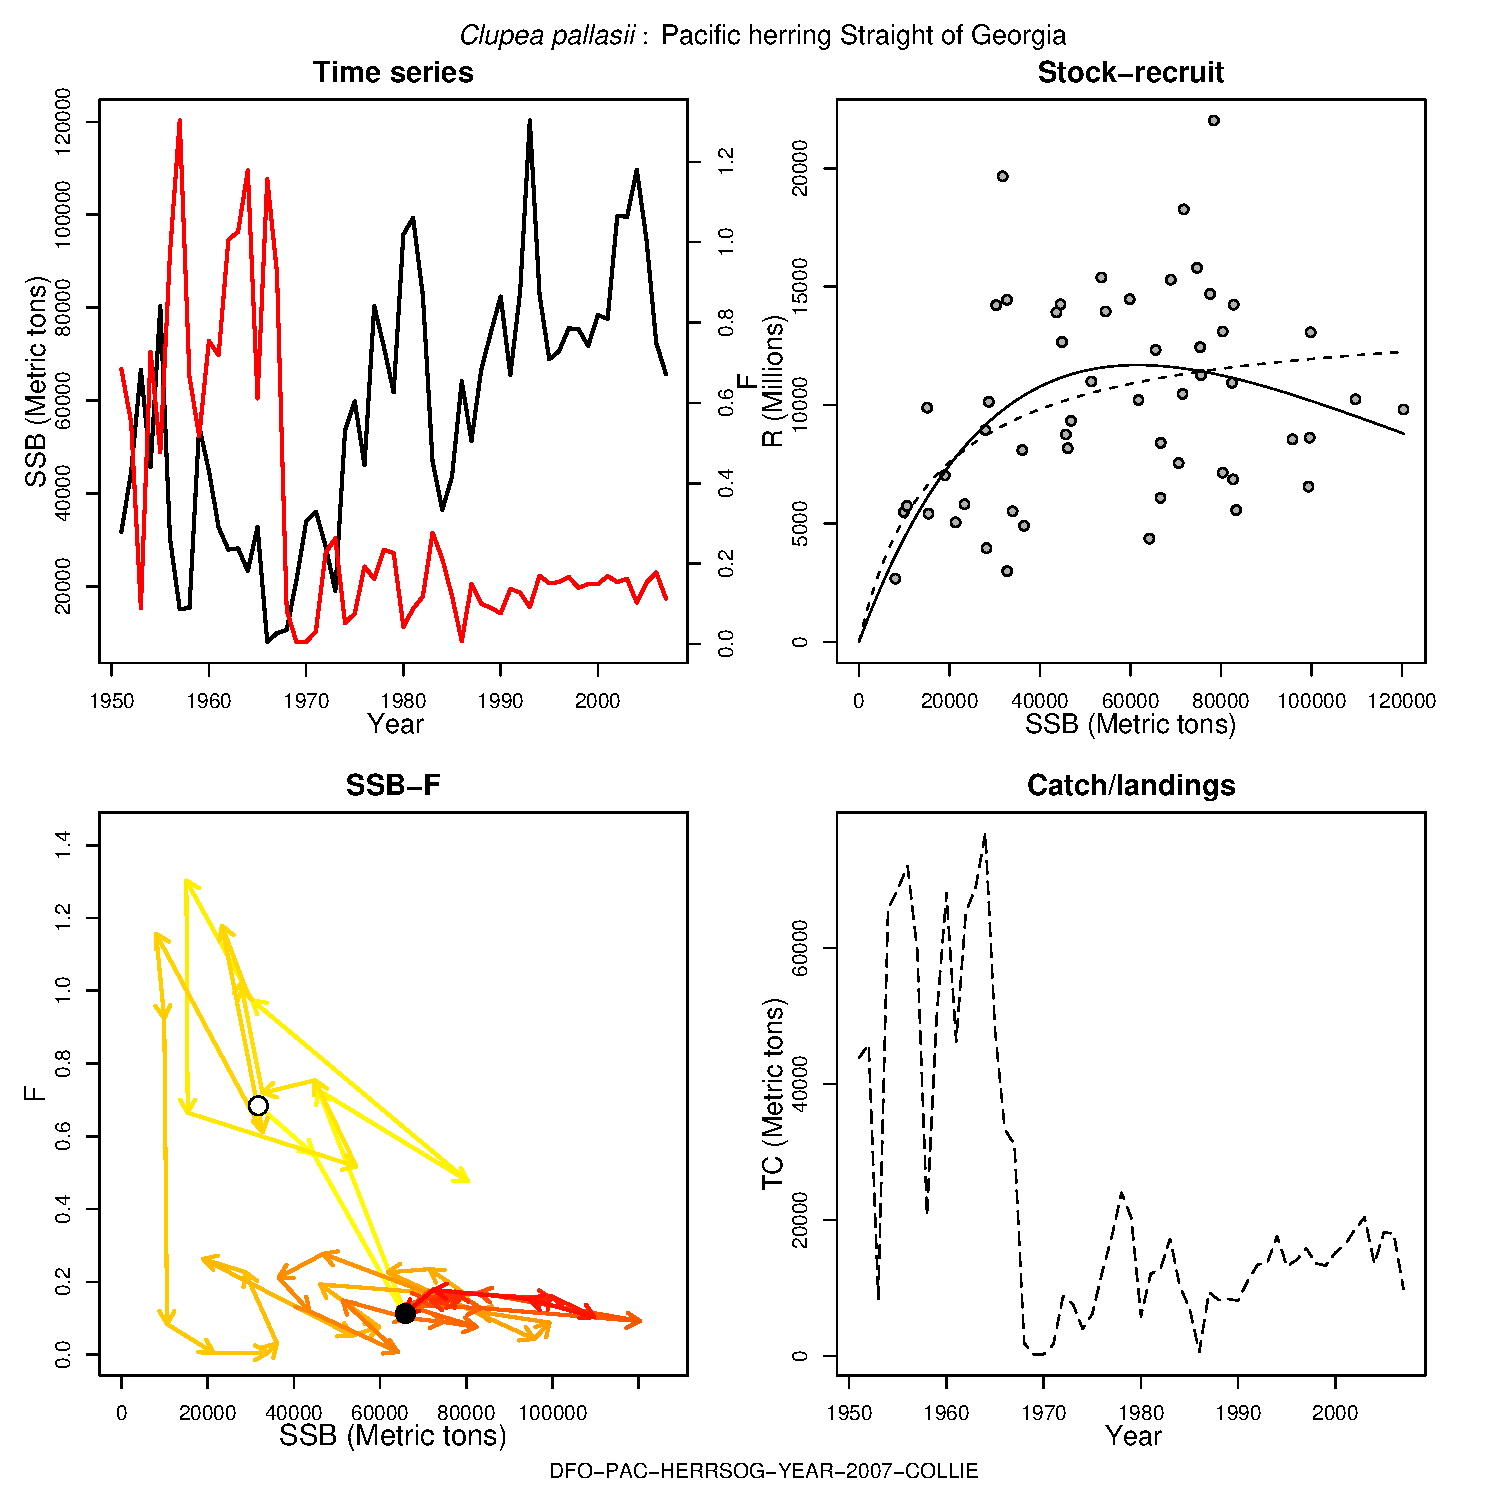
\includegraphics[width=1.2\textwidth]{../R/figures/DFO-PAC-HERRSOG-YEAR-2007-COLLIE.pdf}
\end{center}

\subsubsection{Clupea pallasii - Pacific herring}\index{Pacific herring}\index{Clupea pallasii}\index{Clupeidae!Clupea pallasii}
\begin{center}
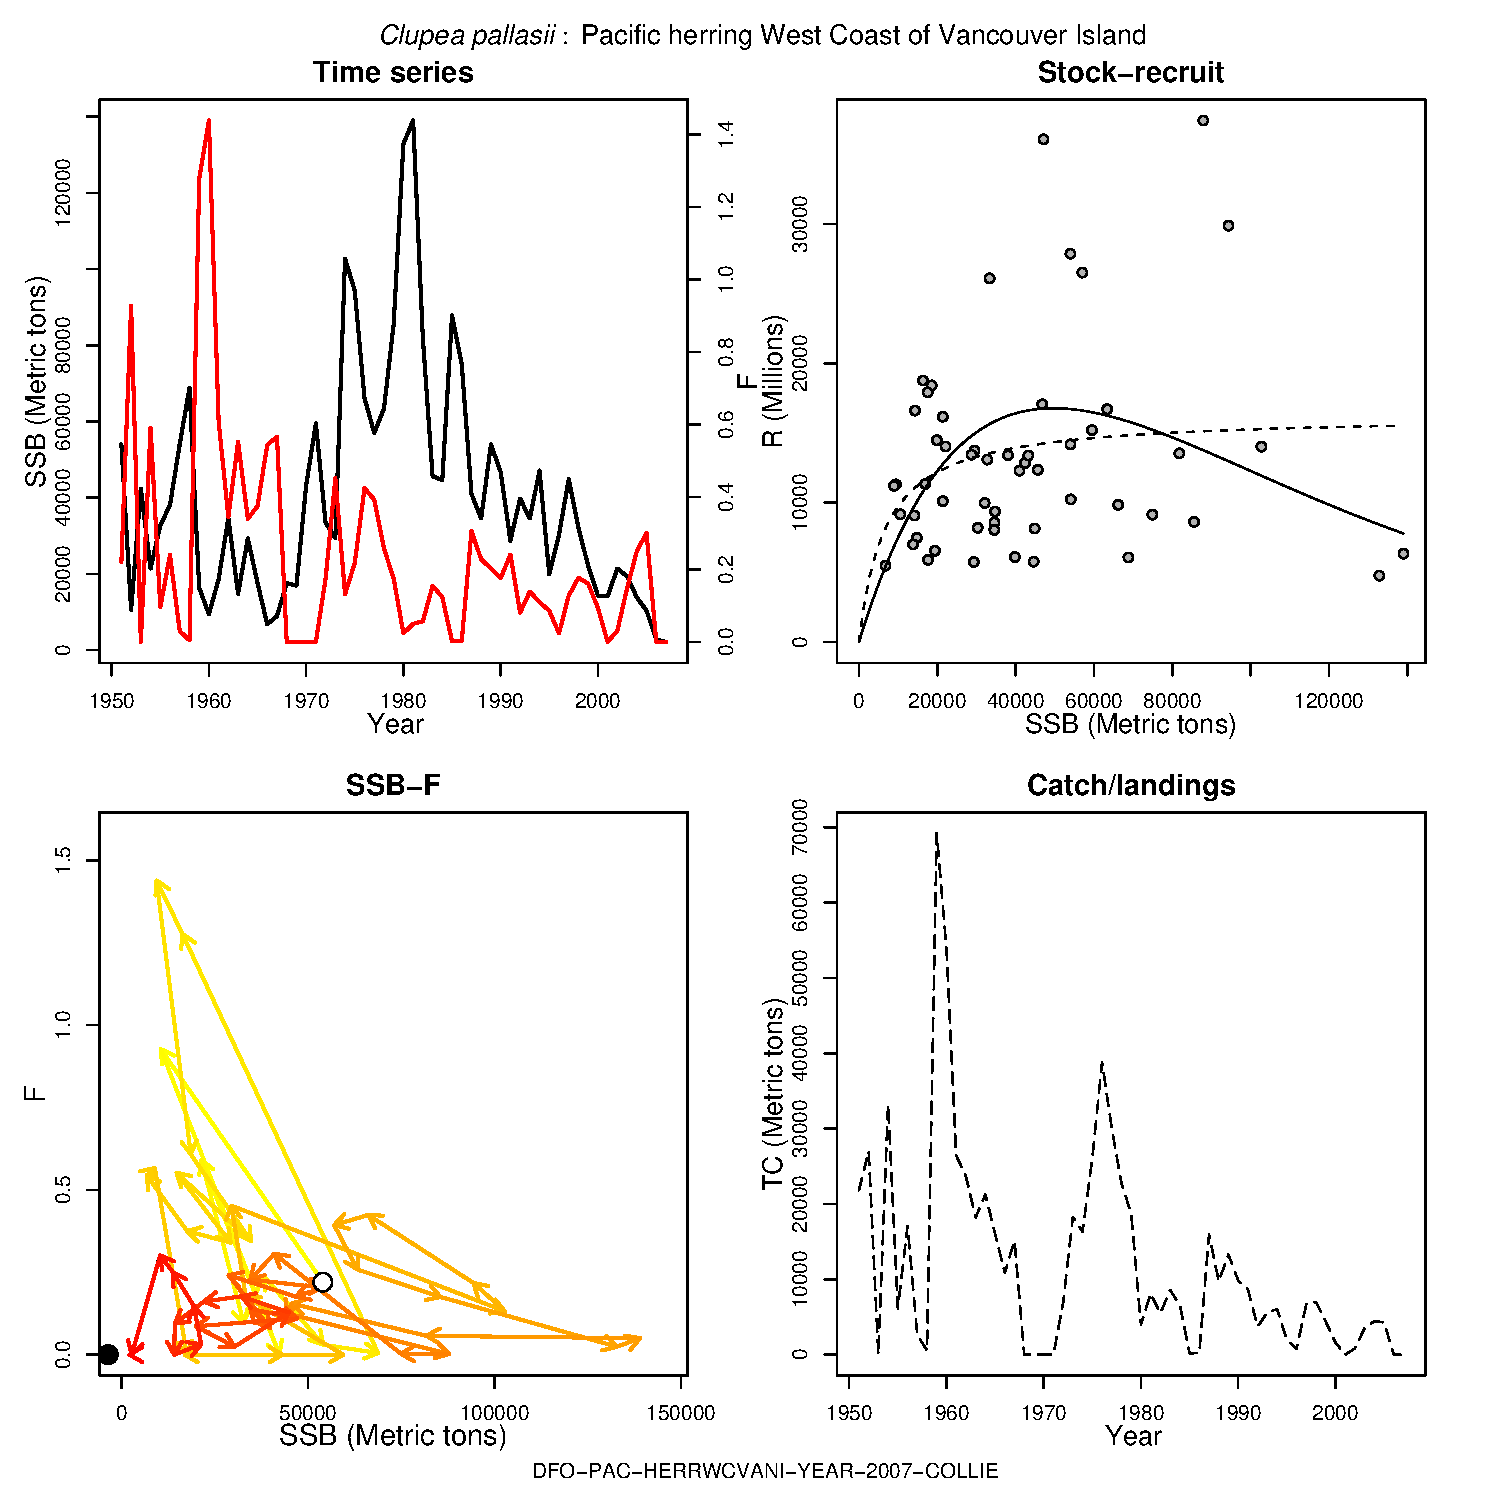
\includegraphics[width=1.2\textwidth]{../R/figures/DFO-PAC-HERRWCVANI-YEAR-2007-COLLIE.pdf}
\end{center}

\subsubsection{Sprattus sprattus - Sprat}\index{Sprat}\index{Sprattus sprattus}\index{Clupeidae!Sprattus sprattus}
\begin{center}
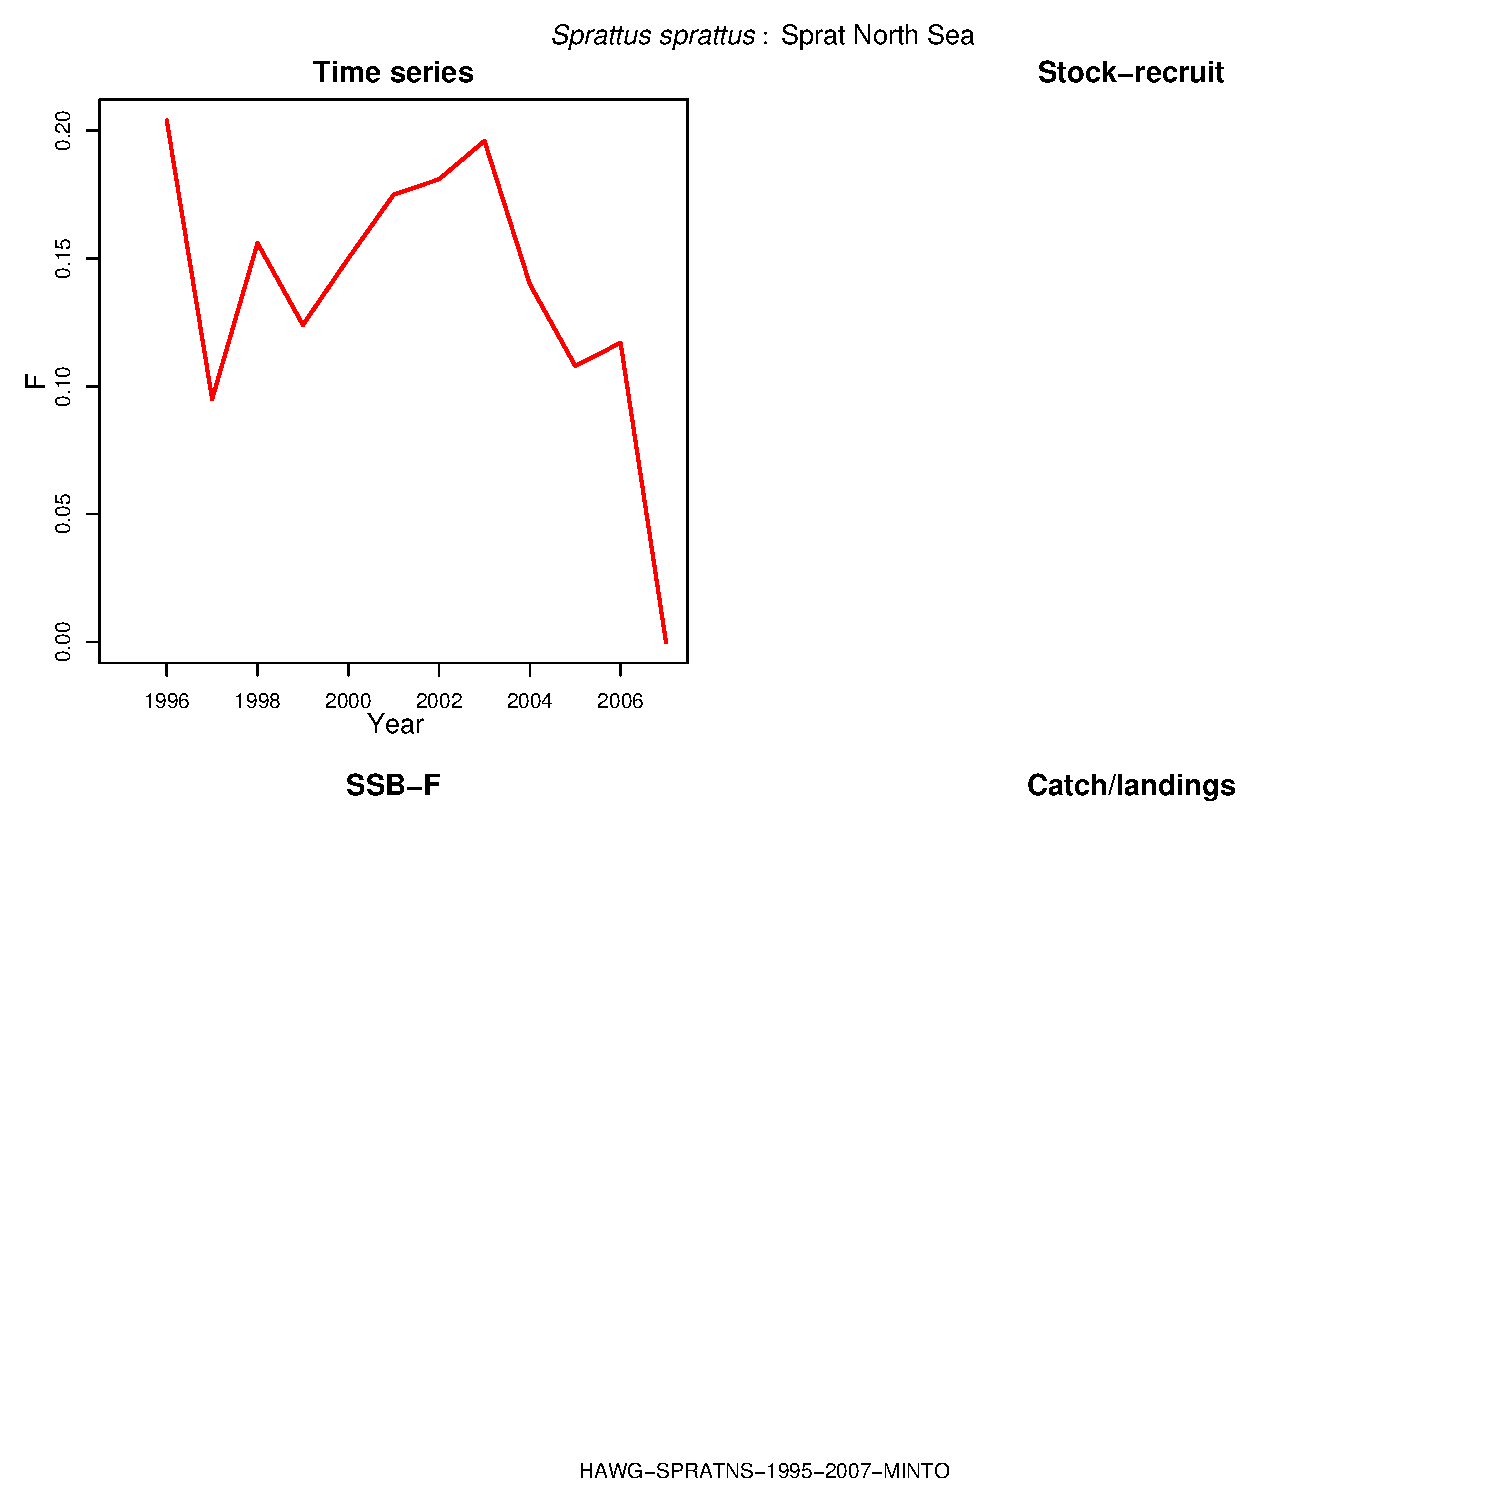
\includegraphics[width=1.2\textwidth]{../R/figures/HAWG-SPRATNS-1995-2007-MINTO.pdf}
\end{center}

\section{Decapoda}\index{Decapoda}

\subsection{Lithodidae}\index{Lithodidae}\index{Decapoda!Lithodidae}

\subsection{Nephropidae}\index{Nephropidae}\index{Decapoda!Nephropidae}

\subsubsection{Homarus americanus - American lobster}\index{American lobster}\index{Homarus americanus}\index{Nephropidae!Homarus americanus}
\begin{center}
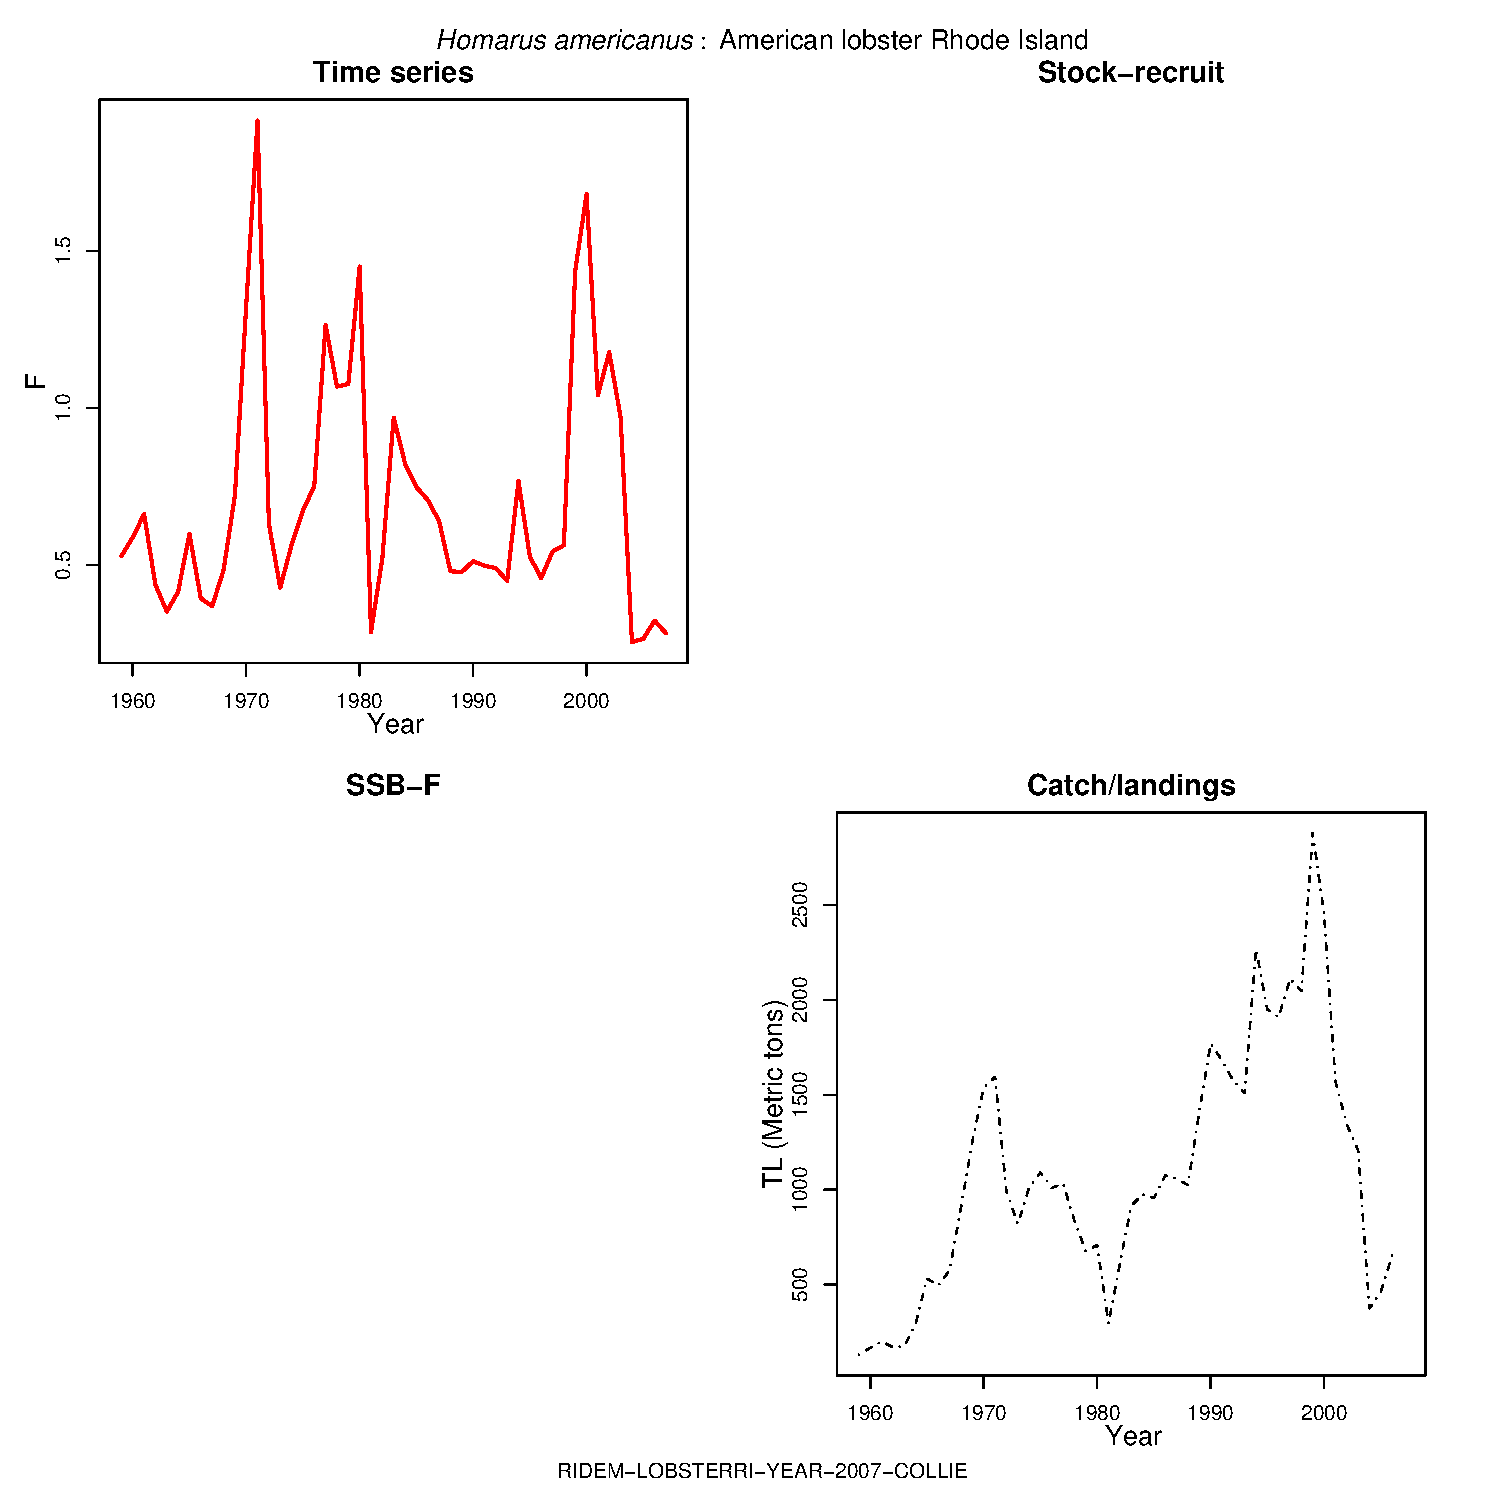
\includegraphics[width=1.2\textwidth]{../R/figures/RIDEM-LOBSTERRI-YEAR-2007-COLLIE.pdf}
\end{center}

\subsection{Oregoniidae}\index{Oregoniidae}\index{Decapoda!Oregoniidae}

\subsubsection{Chionoecetes opilio - Snow crab}\index{Snow crab}\index{Chionoecetes opilio}\index{Oregoniidae!Chionoecetes opilio}
\begin{center}
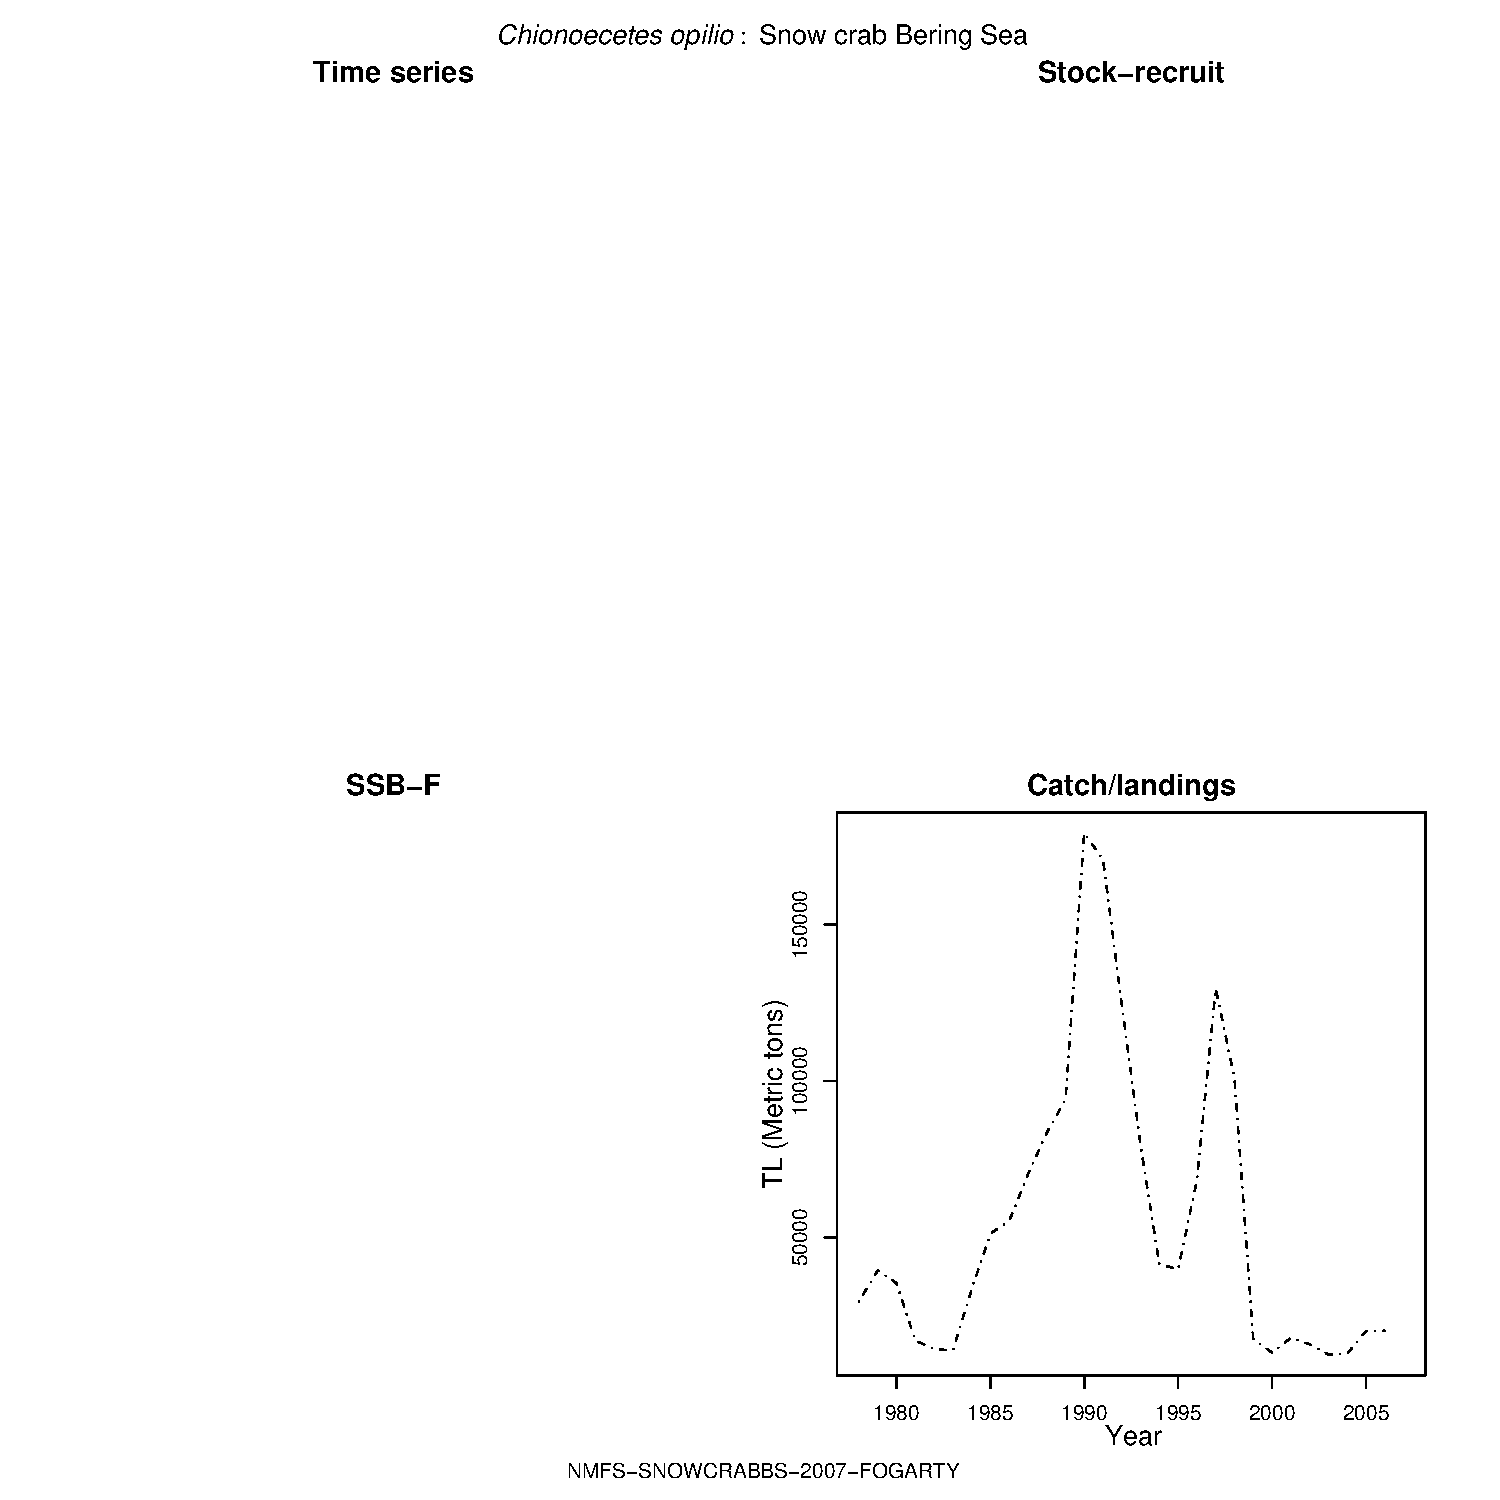
\includegraphics[width=1.2\textwidth]{../R/figures/NMFS-SNOWCRABBS-2007-FOGARTY.pdf}
\end{center}

\section{Gadiformes}\index{Gadiformes}

\subsection{Gadidae}\index{Gadidae}\index{Gadiformes!Gadidae}

\subsubsection{Gadus macrocephalus - Pacific cod}\index{Pacific cod}\index{Gadus macrocephalus}\index{Gadidae!Gadus macrocephalus}
\begin{center}
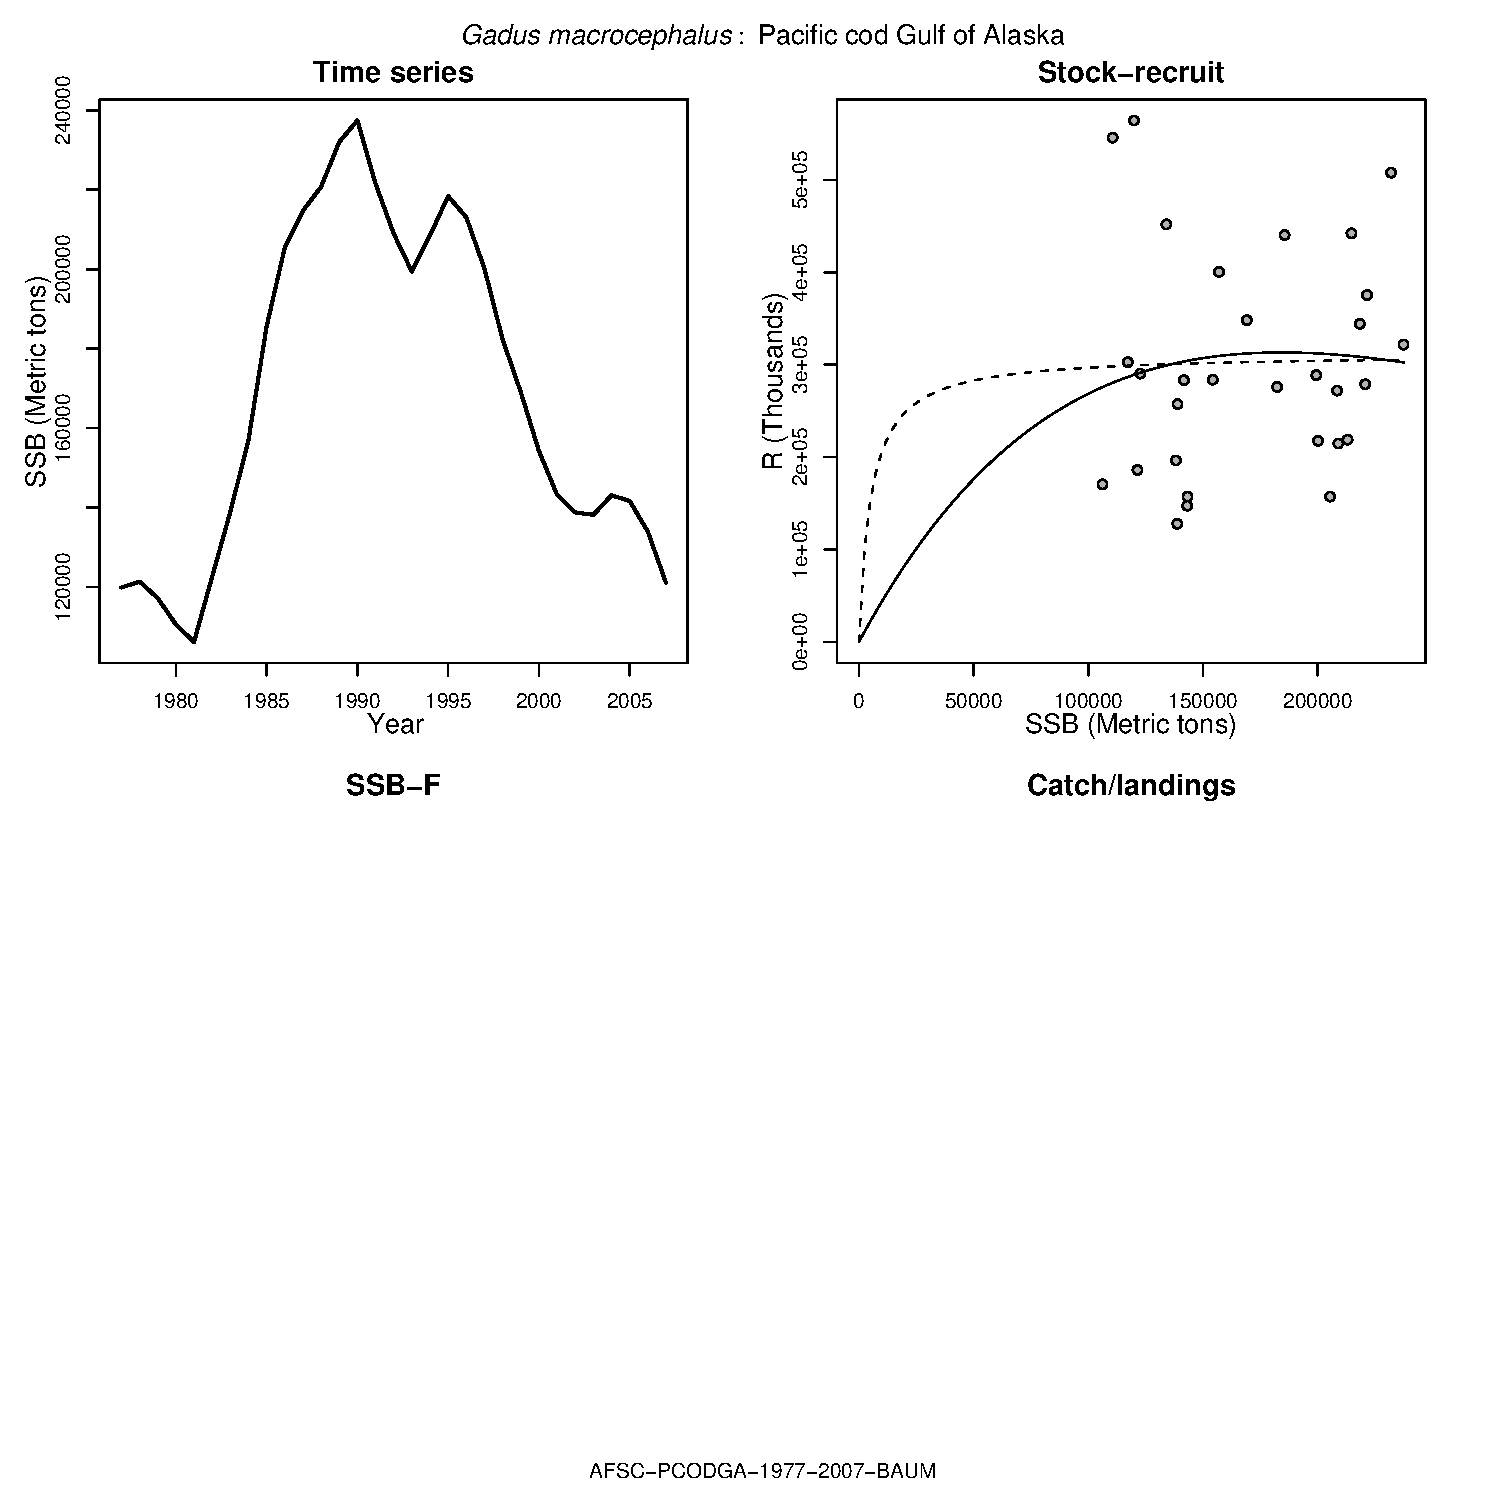
\includegraphics[width=1.2\textwidth]{../R/figures/AFSC-PCODGA-1977-2007-BAUM.pdf}
\end{center}

\subsubsection{Gadus macrocephalus - Pacific cod}\index{Pacific cod}\index{Gadus macrocephalus}\index{Gadidae!Gadus macrocephalus}
\begin{center}
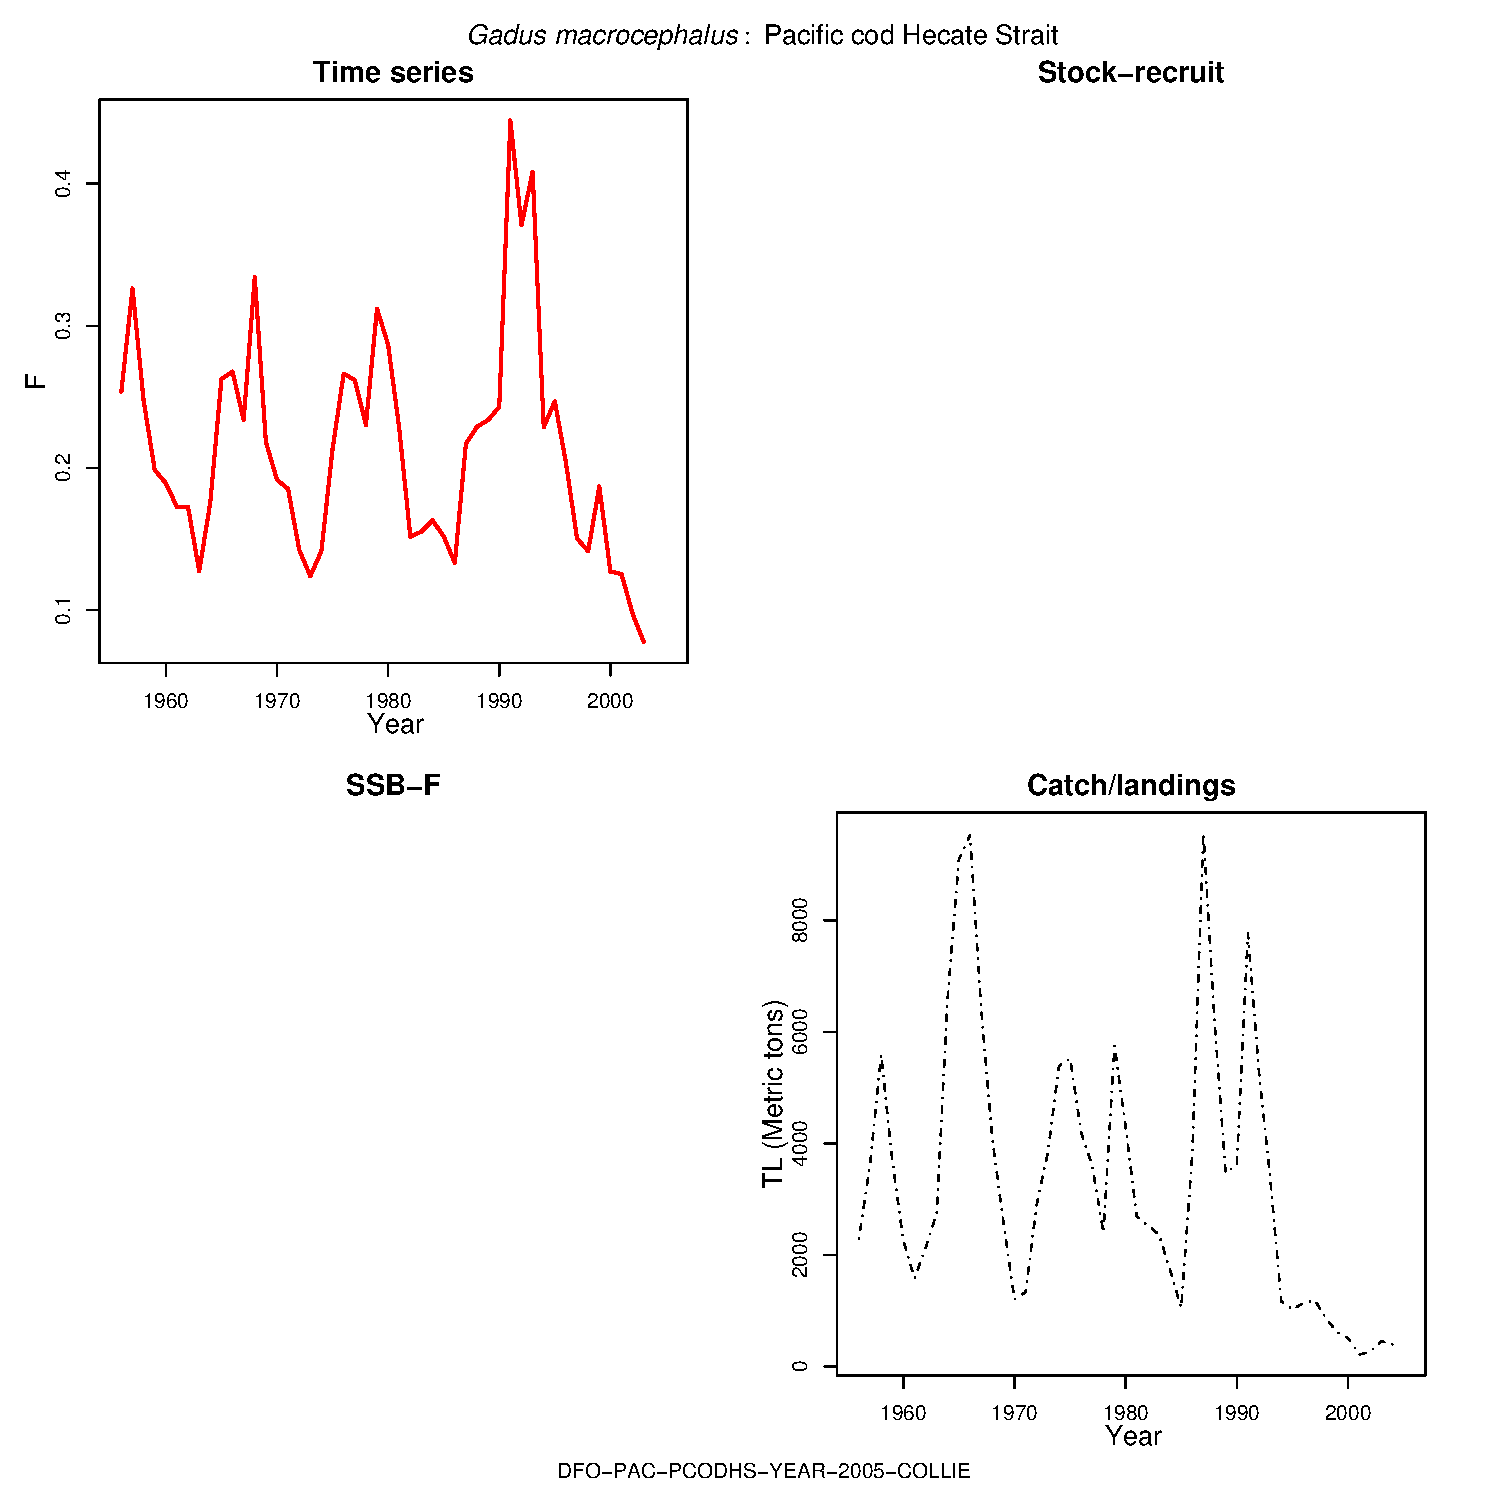
\includegraphics[width=1.2\textwidth]{../R/figures/DFO-PAC-PCODHS-YEAR-2005-COLLIE.pdf}
\end{center}

\subsubsection{Gadus macrocephalus - Pacific cod}\index{Pacific cod}\index{Gadus macrocephalus}\index{Gadidae!Gadus macrocephalus}
\begin{center}
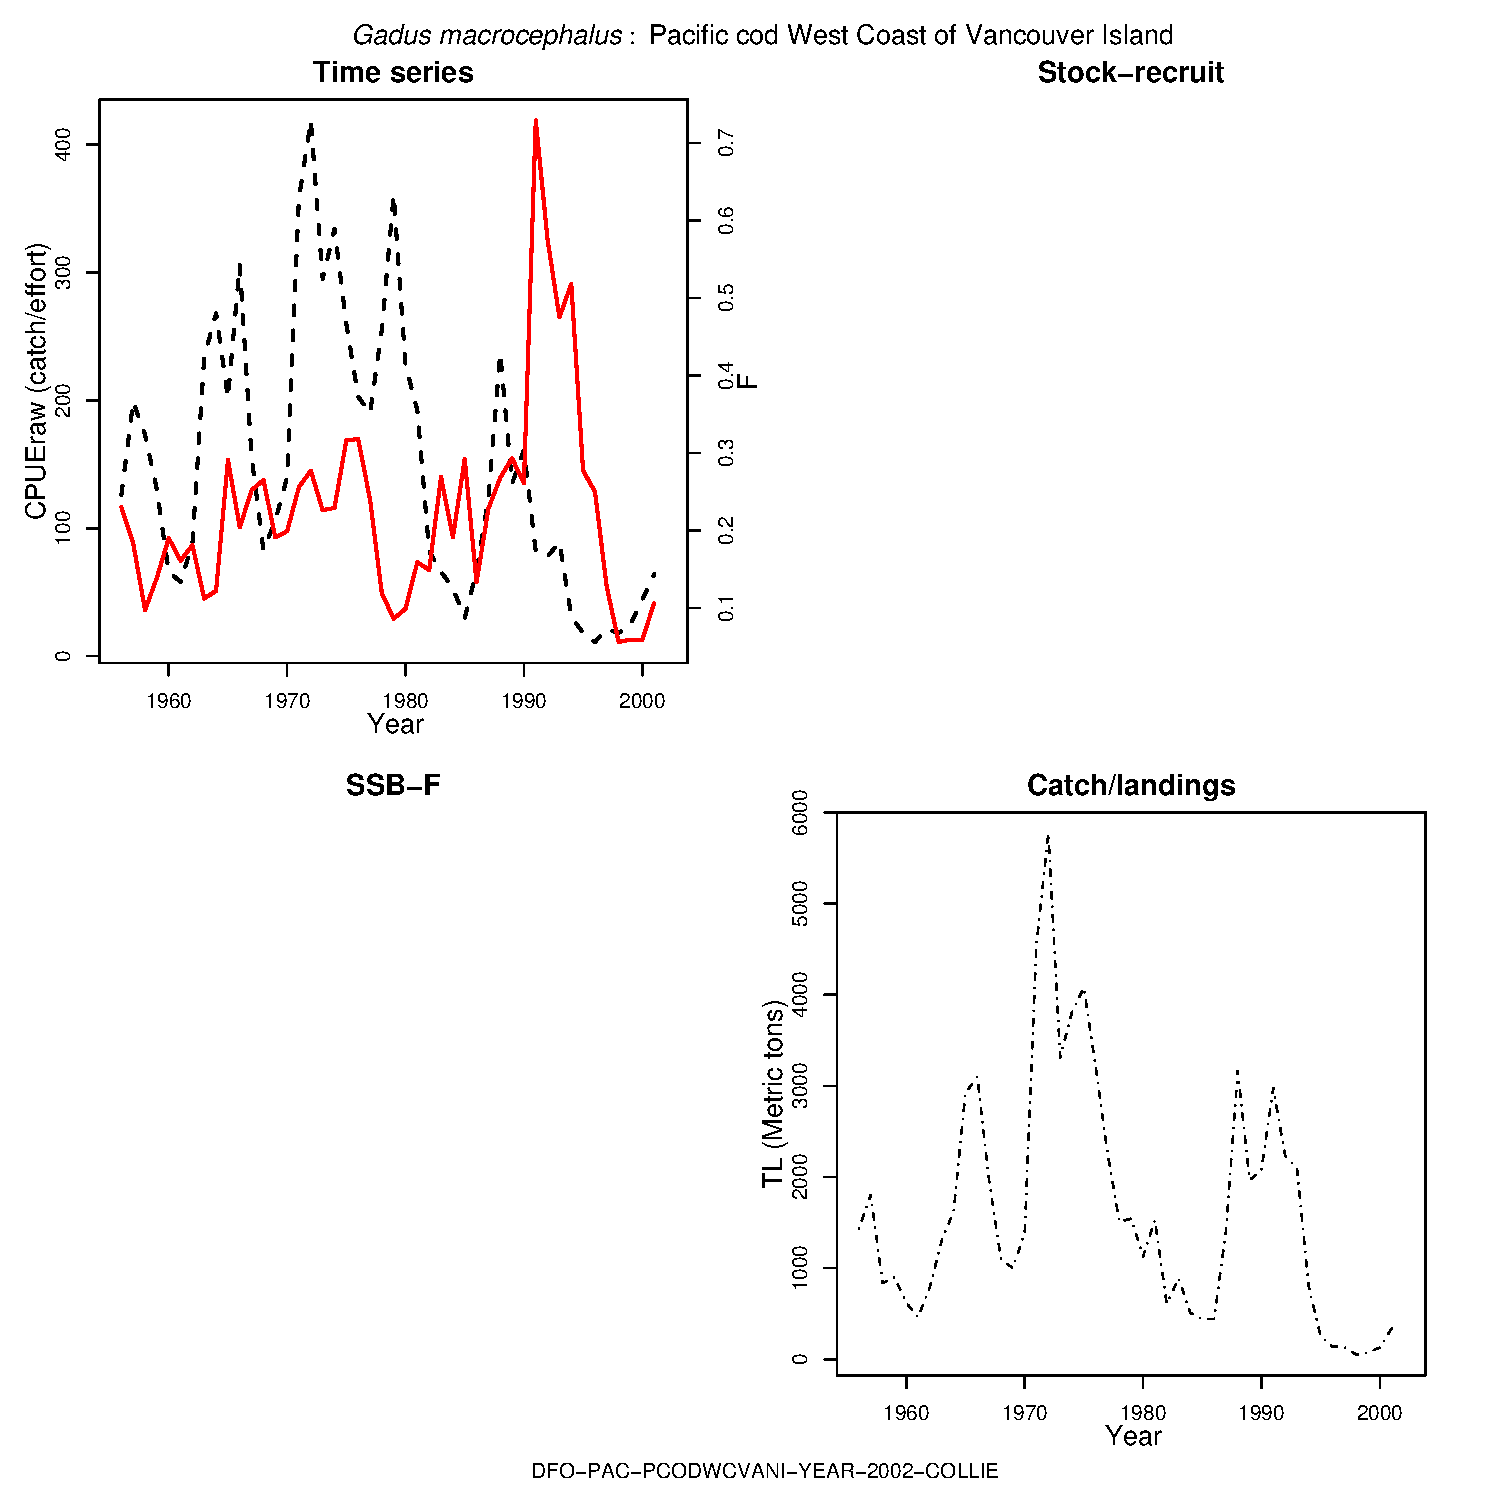
\includegraphics[width=1.2\textwidth]{../R/figures/DFO-PAC-PCODWCVANI-YEAR-2002-COLLIE.pdf}
\end{center}

\subsubsection{Gadus macrocephalus - Pacific cod}\index{Pacific cod}\index{Gadus macrocephalus}\index{Gadidae!Gadus macrocephalus}
\begin{center}
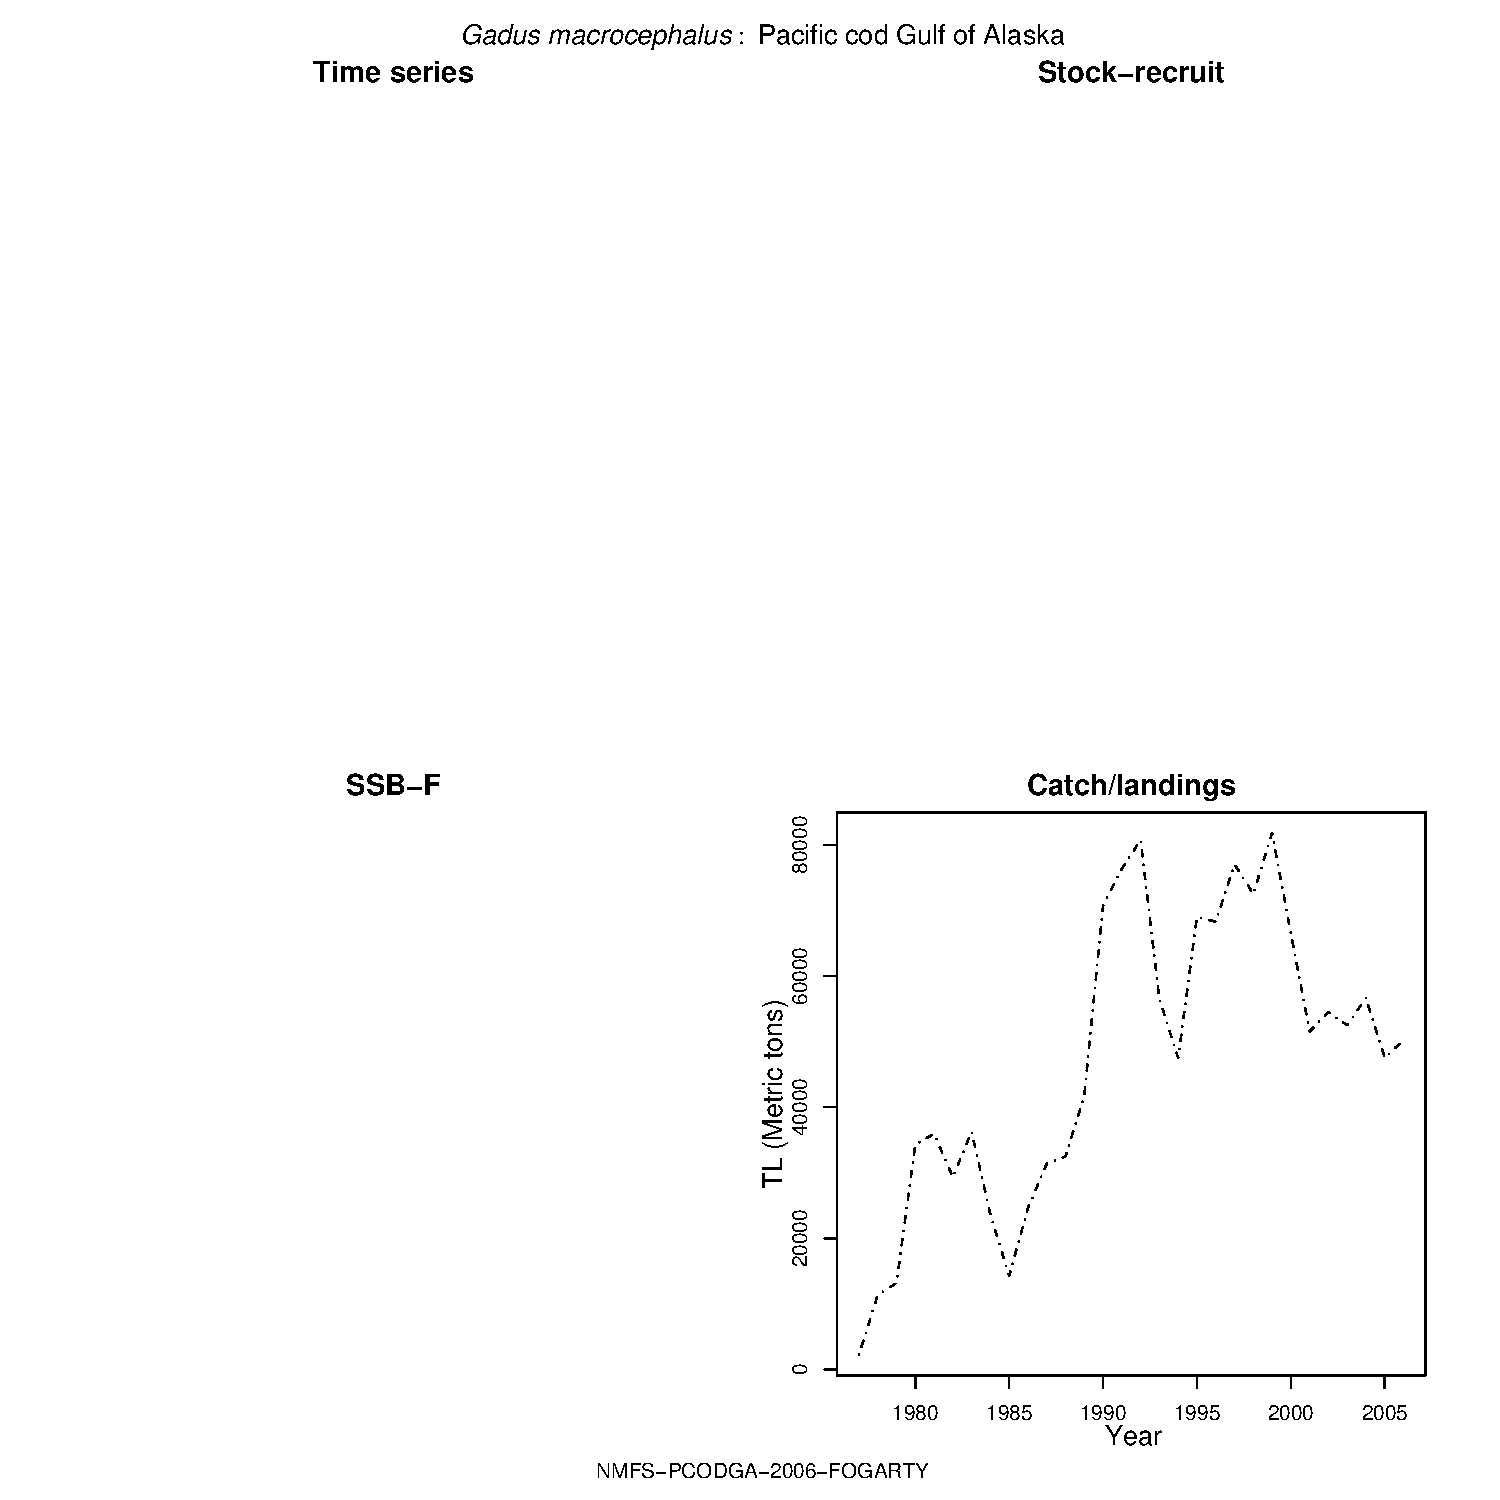
\includegraphics[width=1.2\textwidth]{../R/figures/NMFS-PCODGA-2006-FOGARTY.pdf}
\end{center}

\subsubsection{Gadus macrocephalus - Pacific cod}\index{Pacific cod}\index{Gadus macrocephalus}\index{Gadidae!Gadus macrocephalus}
\begin{center}
\includegraphics[width=1.2\textwidth]{../R/figures/PHONYassessorid-PCODGA-1975-2000-MYERS.pdf}
\end{center}

\subsubsection{Gadus macrocephalus - Pacific cod}\index{Pacific cod}\index{Gadus macrocephalus}\index{Gadidae!Gadus macrocephalus}
\begin{center}
\includegraphics[width=1.2\textwidth]{../R/figures/PHONYassessorid-PCODHS-1956-1989-MYERS.pdf}
\end{center}

\subsubsection{Gadus morhua - Atlantic cod}\index{Atlantic cod}\index{Gadus morhua}\index{Gadidae!Gadus morhua}
\begin{center}
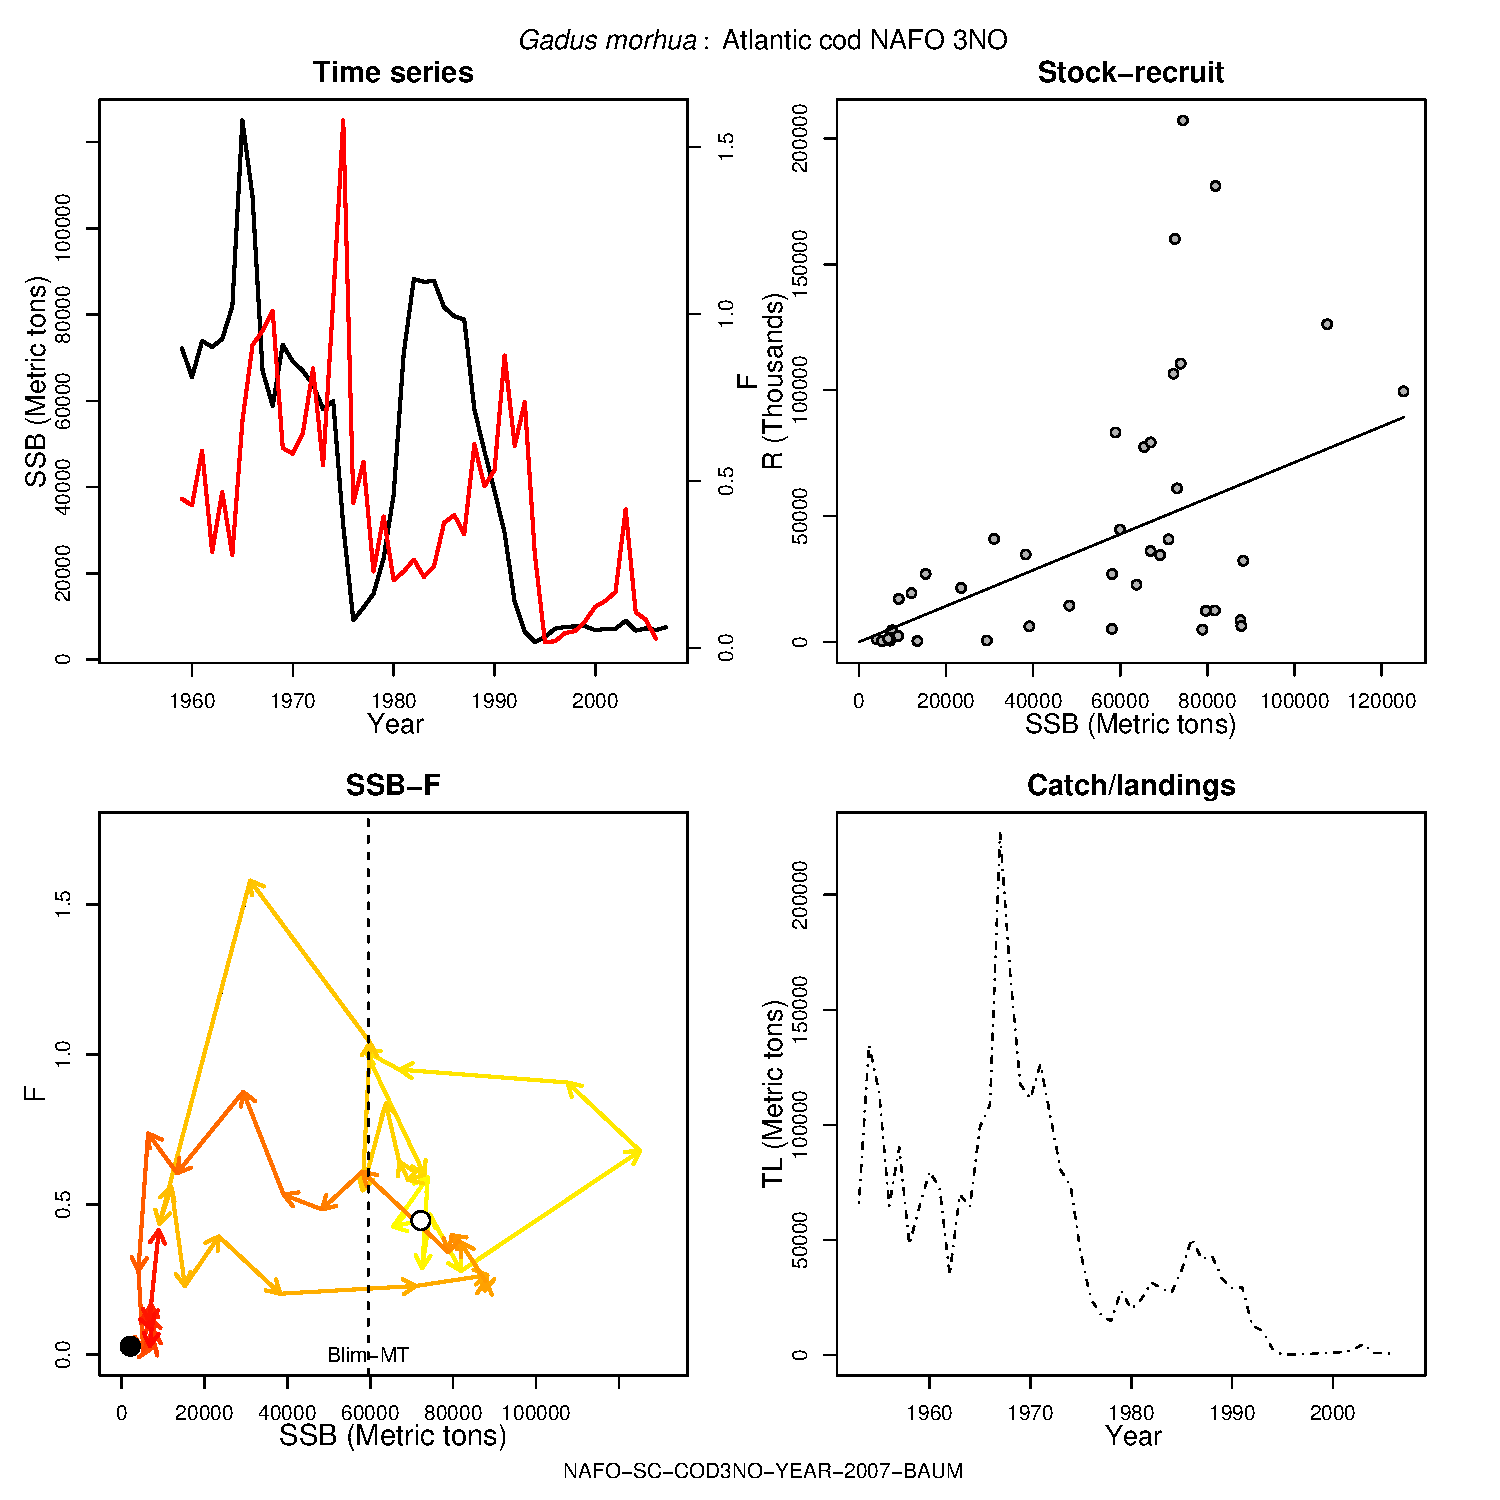
\includegraphics[width=1.2\textwidth]{../R/figures/NAFO-SC-COD3NO-YEAR-2007-BAUM.pdf}
\end{center}

\subsubsection{Gadus morhua - Atlantic cod}\index{Atlantic cod}\index{Gadus morhua}\index{Gadidae!Gadus morhua}
\begin{center}
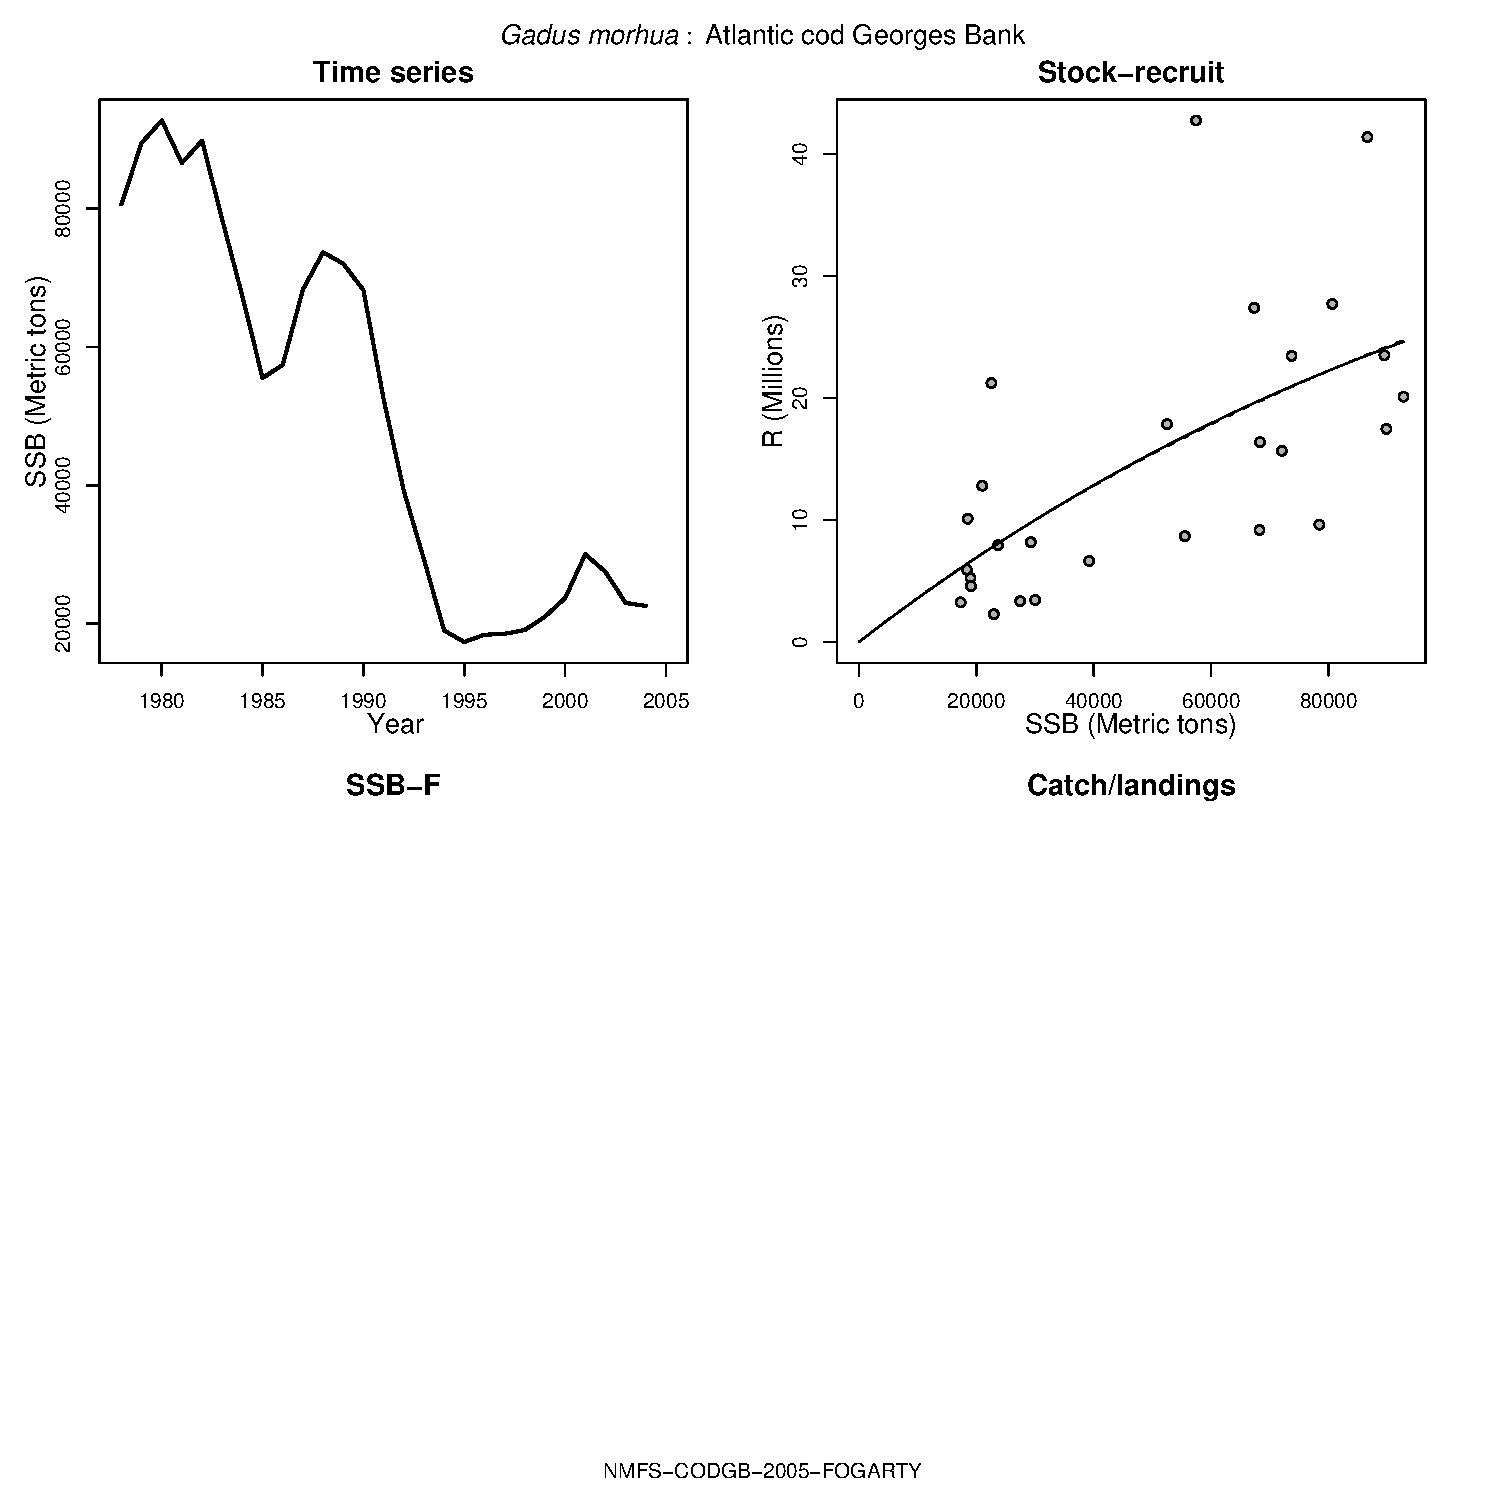
\includegraphics[width=1.2\textwidth]{../R/figures/NMFS-CODGB-2005-FOGARTY.pdf}
\end{center}

\subsubsection{Gadus morhua - Atlantic cod}\index{Atlantic cod}\index{Gadus morhua}\index{Gadidae!Gadus morhua}
\begin{center}
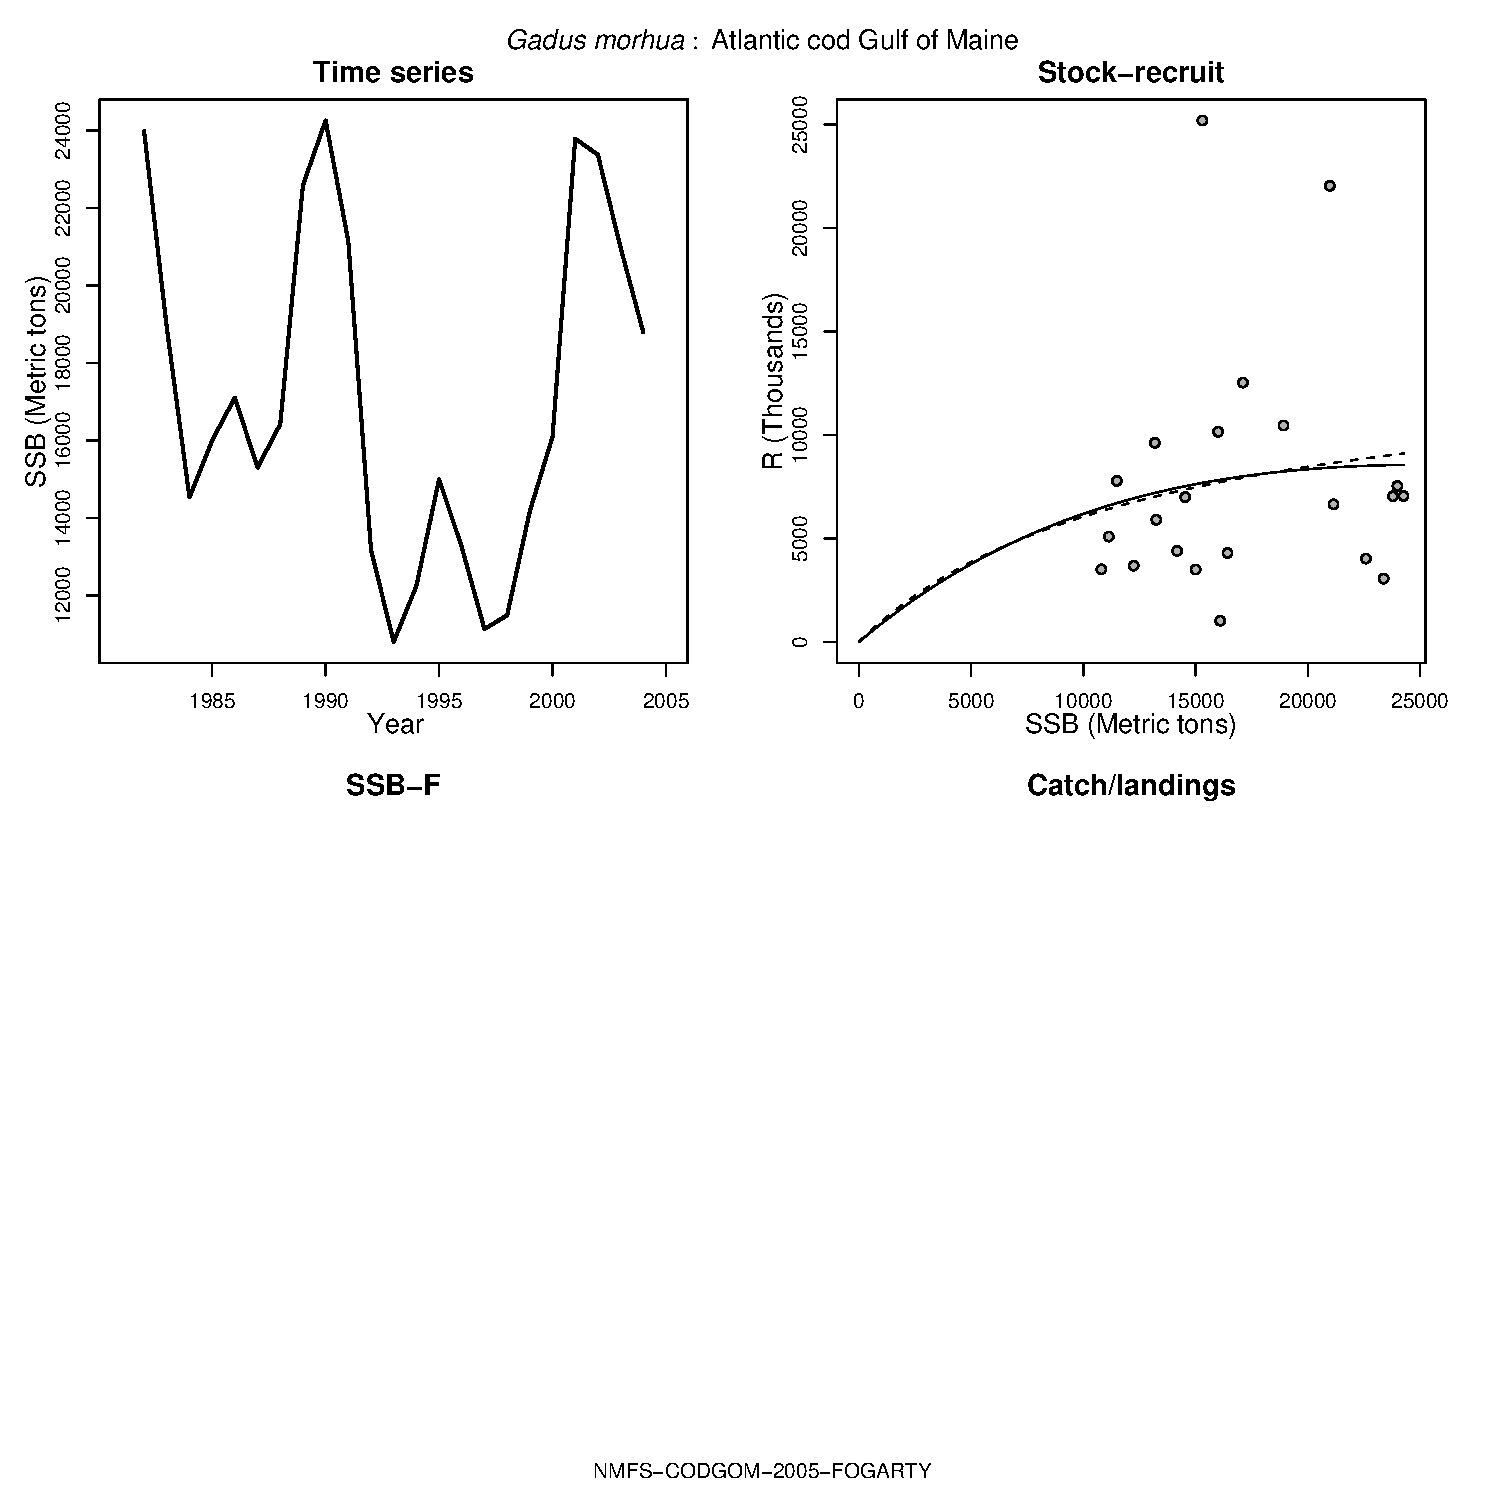
\includegraphics[width=1.2\textwidth]{../R/figures/NMFS-CODGOM-2005-FOGARTY.pdf}
\end{center}

\subsubsection{Gadus morhua - Atlantic cod}\index{Atlantic cod}\index{Gadus morhua}\index{Gadidae!Gadus morhua}
\begin{center}
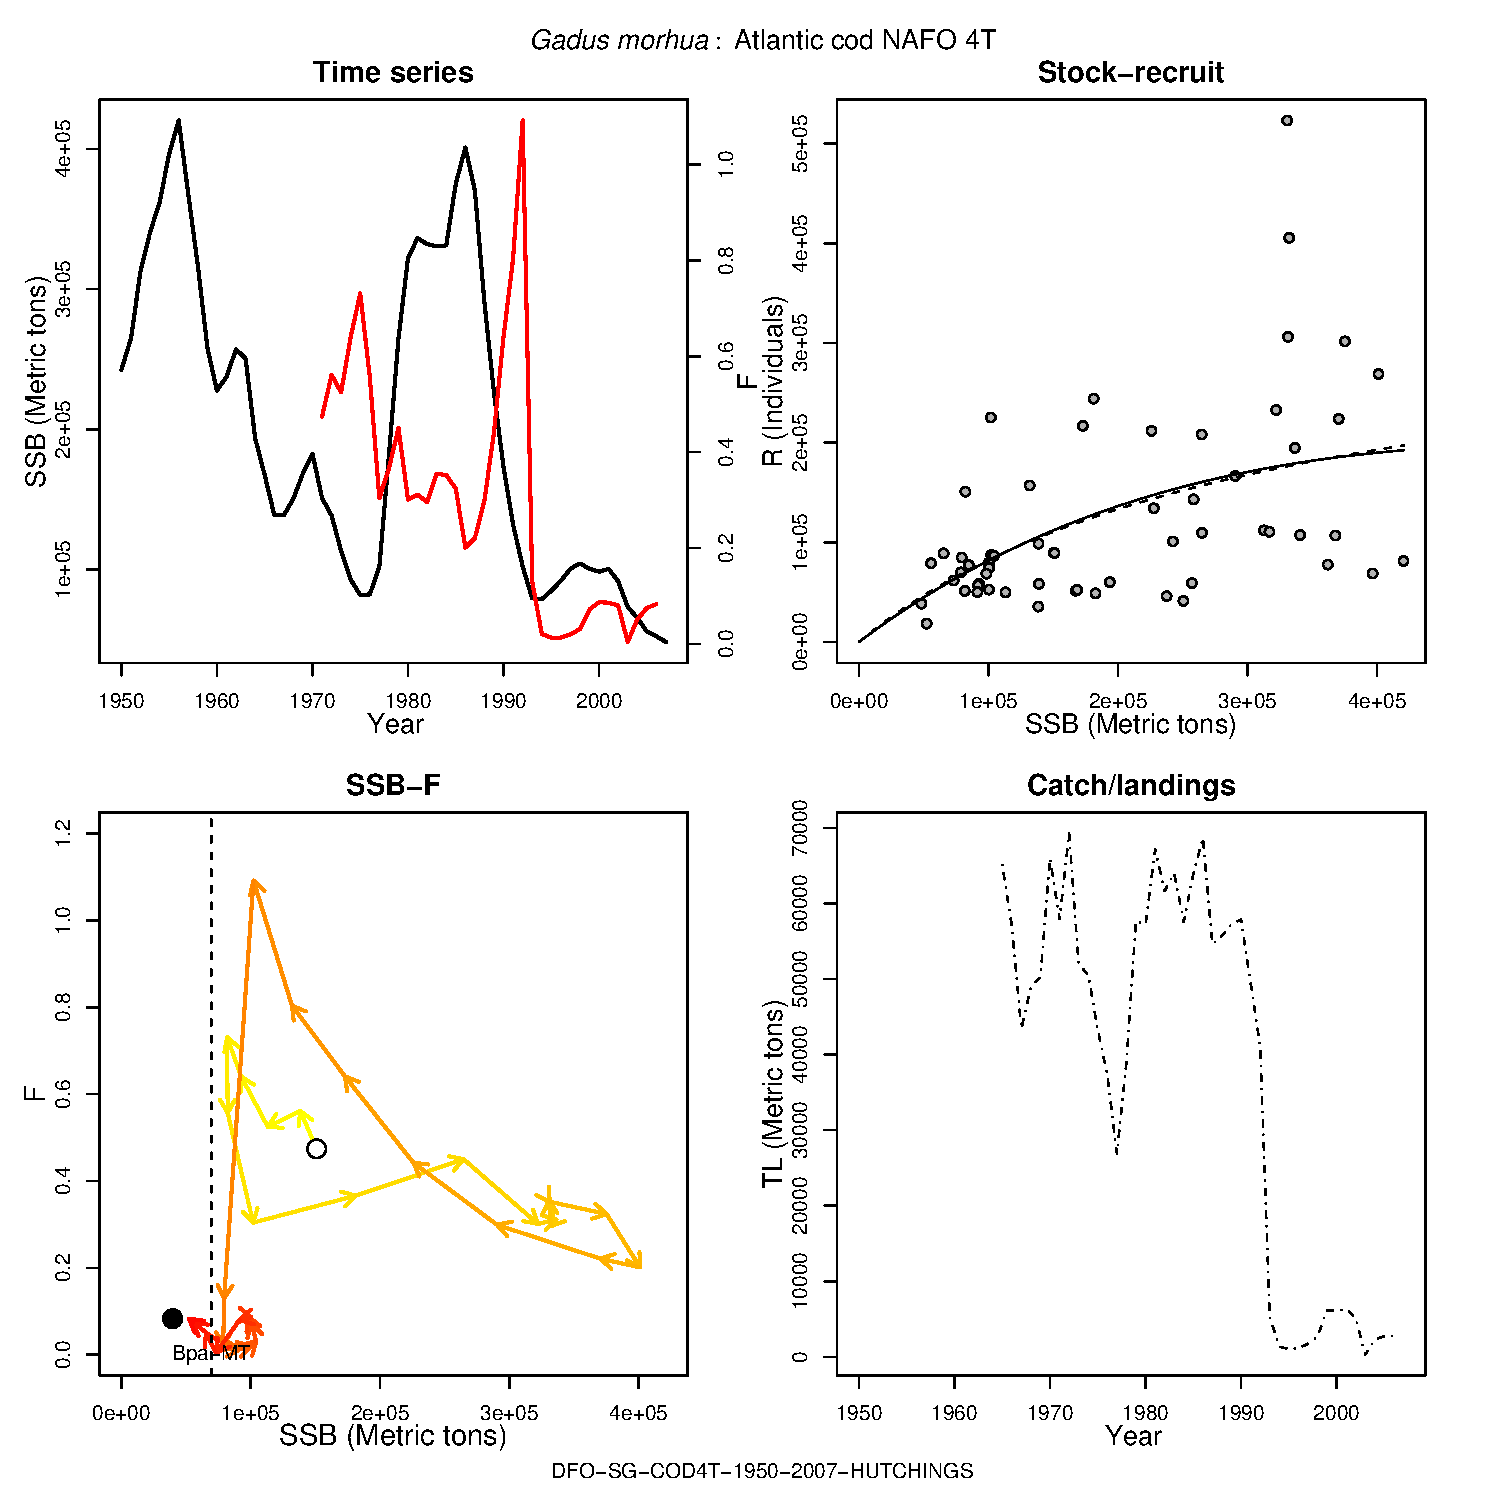
\includegraphics[width=1.2\textwidth]{../R/figures/DFO-SG-COD4T-1950-2007-HUTCHINGS.pdf}
\end{center}

\subsubsection{Gadus morhua - Atlantic cod}\index{Atlantic cod}\index{Gadus morhua}\index{Gadidae!Gadus morhua}
\begin{center}
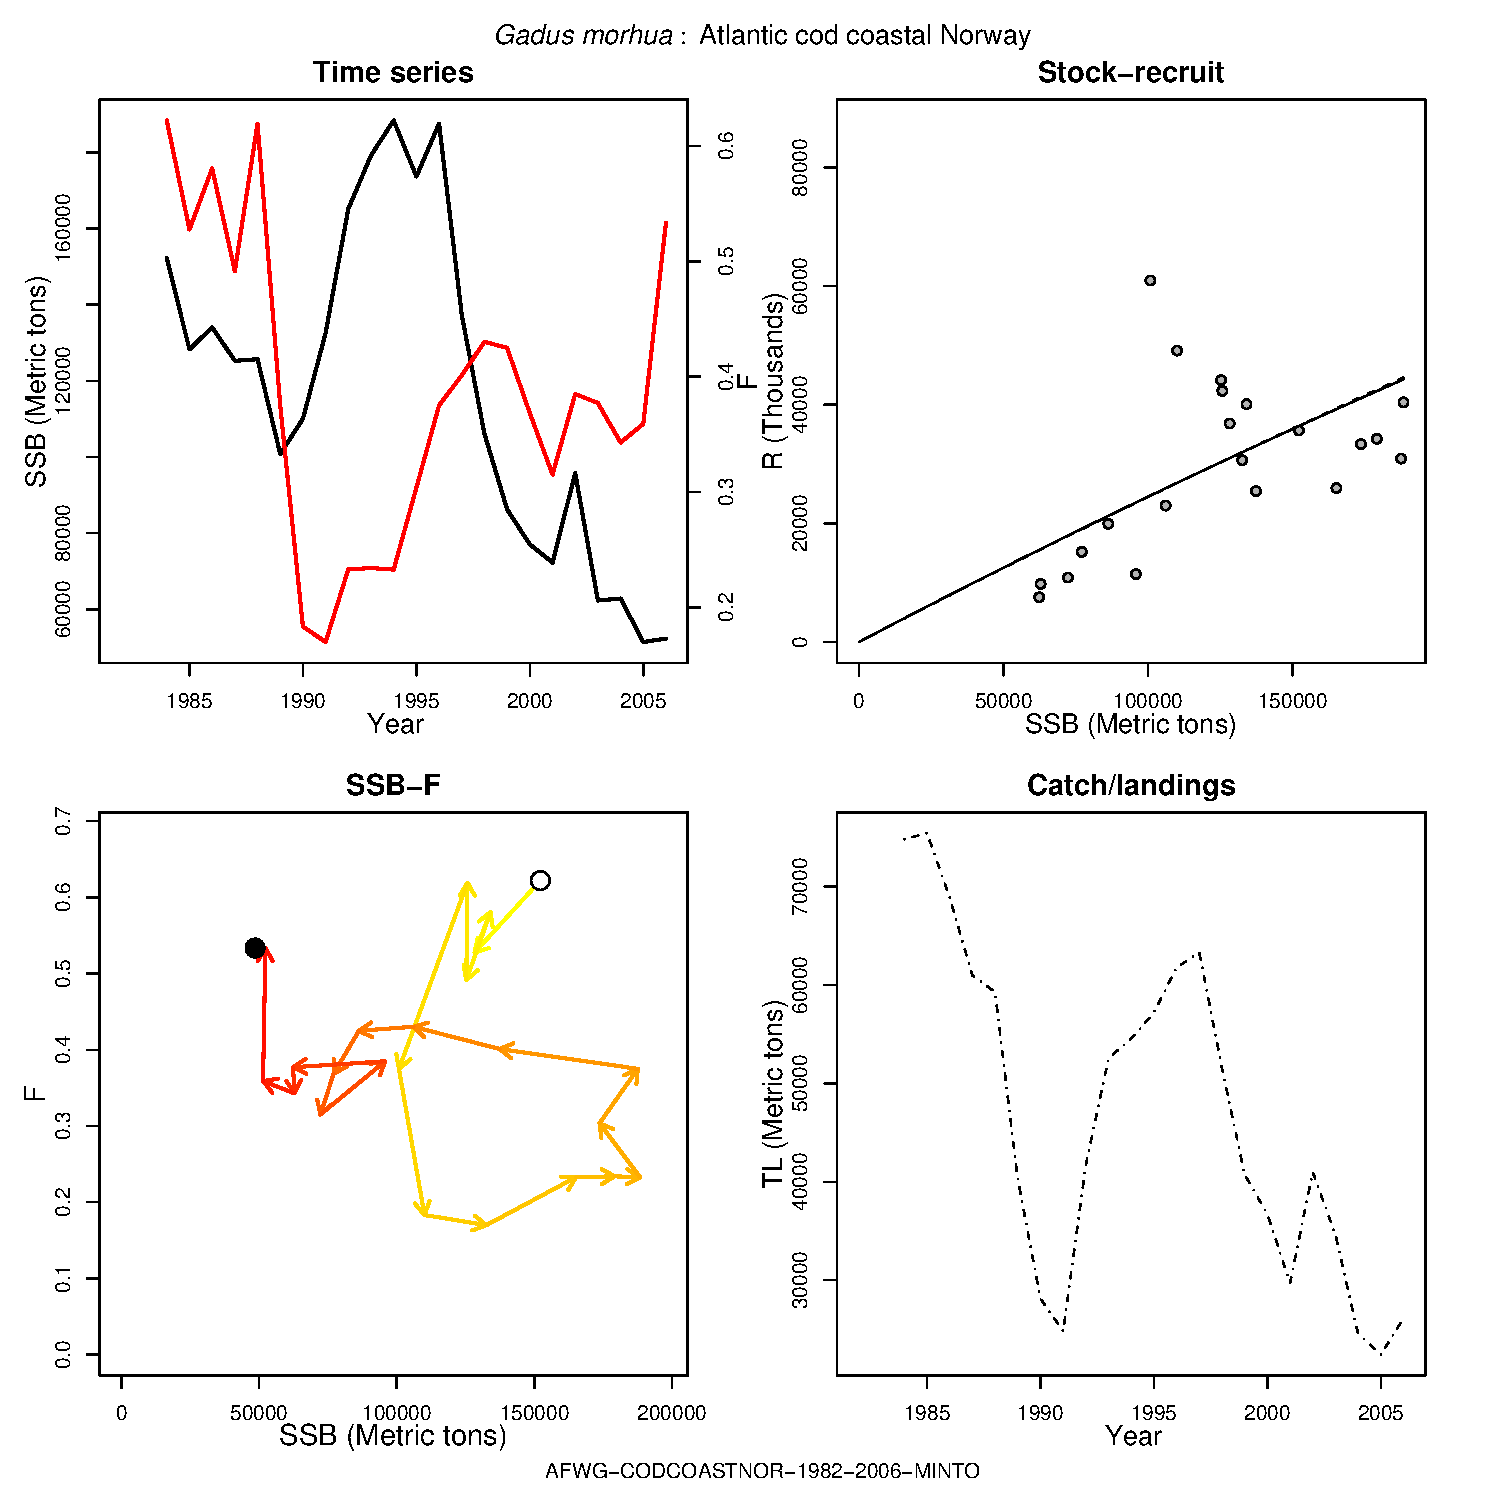
\includegraphics[width=1.2\textwidth]{../R/figures/AFWG-CODCOASTNOR-1982-2006-MINTO.pdf}
\end{center}

\subsubsection{Gadus morhua - Atlantic cod}\index{Atlantic cod}\index{Gadus morhua}\index{Gadidae!Gadus morhua}
\begin{center}
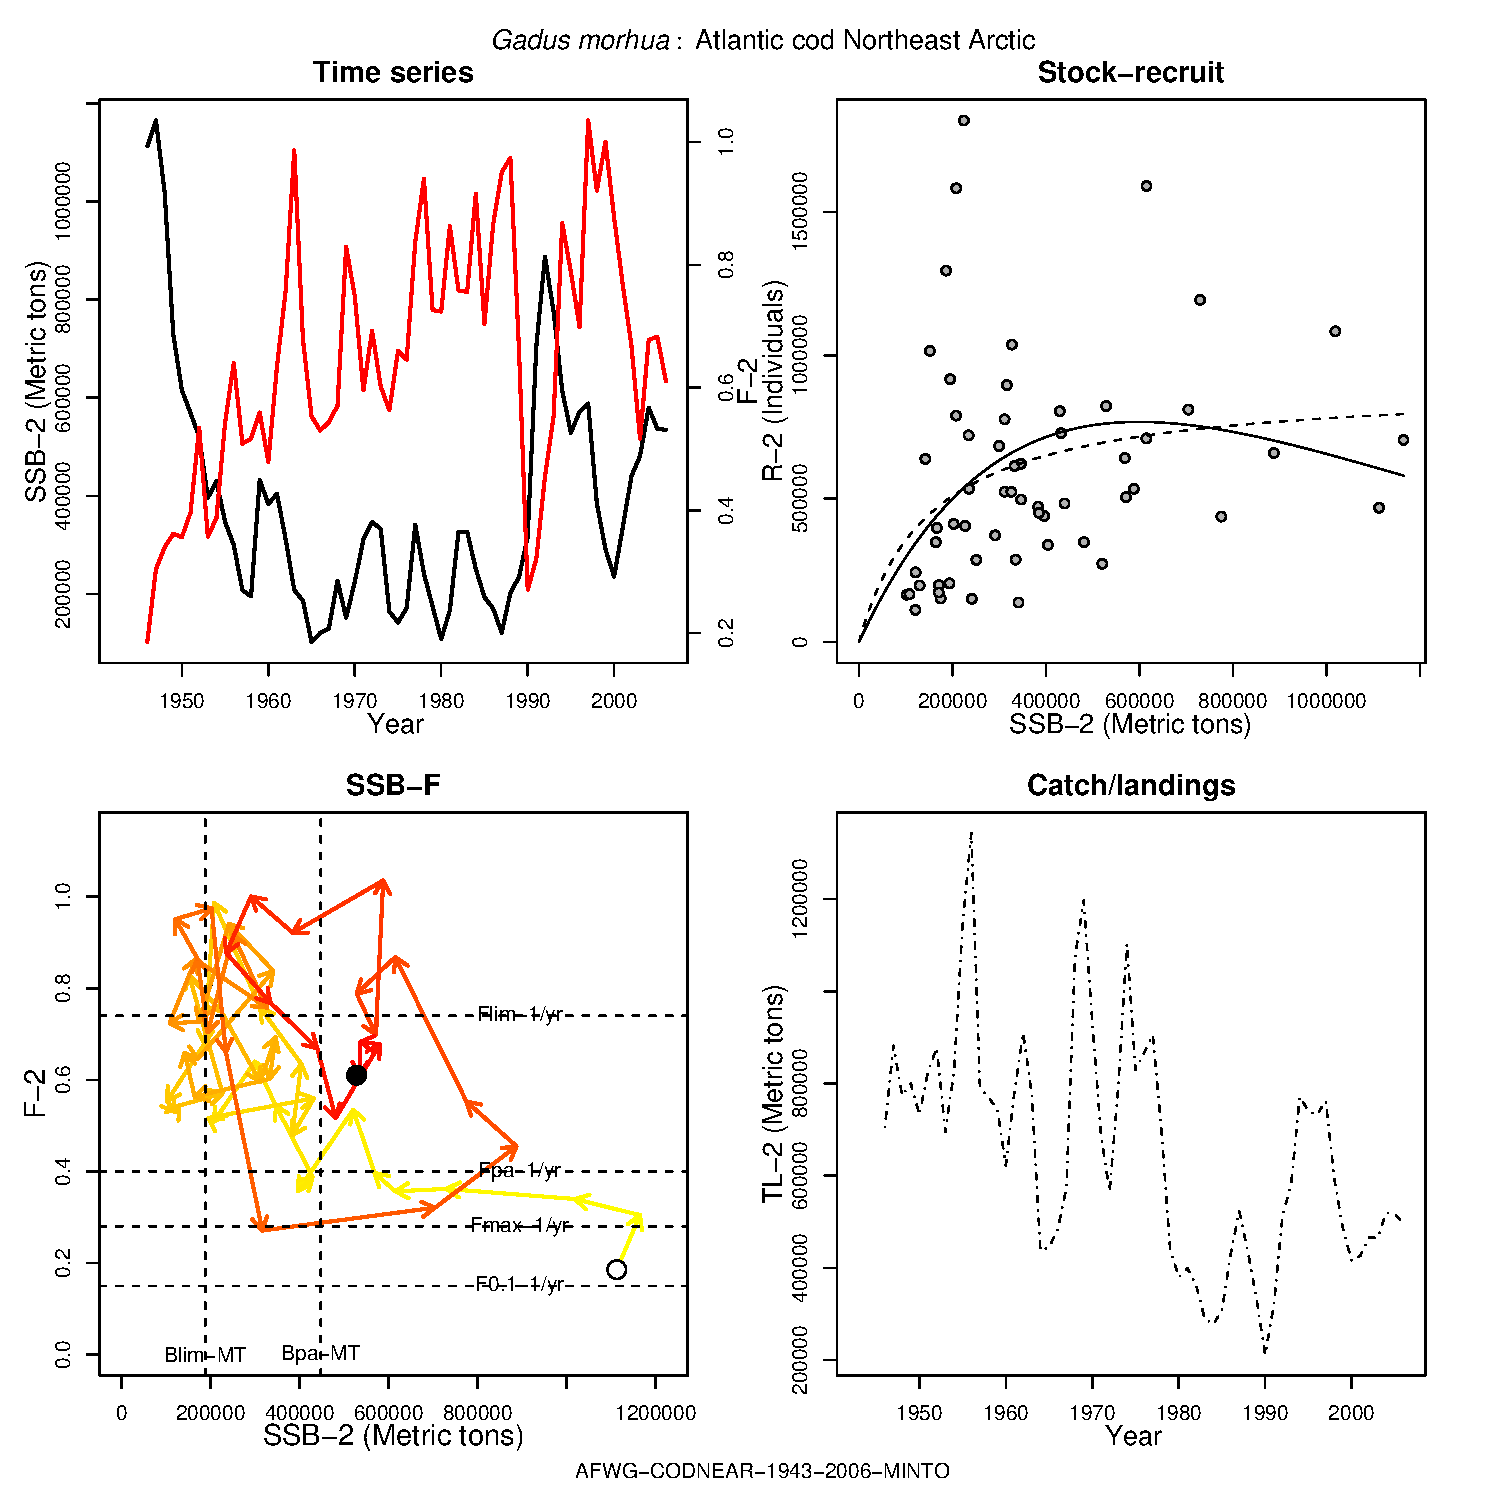
\includegraphics[width=1.2\textwidth]{../R/figures/AFWG-CODNEAR-1943-2006-MINTO.pdf}
\end{center}

\subsubsection{Gadus morhua - Atlantic cod}\index{Atlantic cod}\index{Gadus morhua}\index{Gadidae!Gadus morhua}
\begin{center}
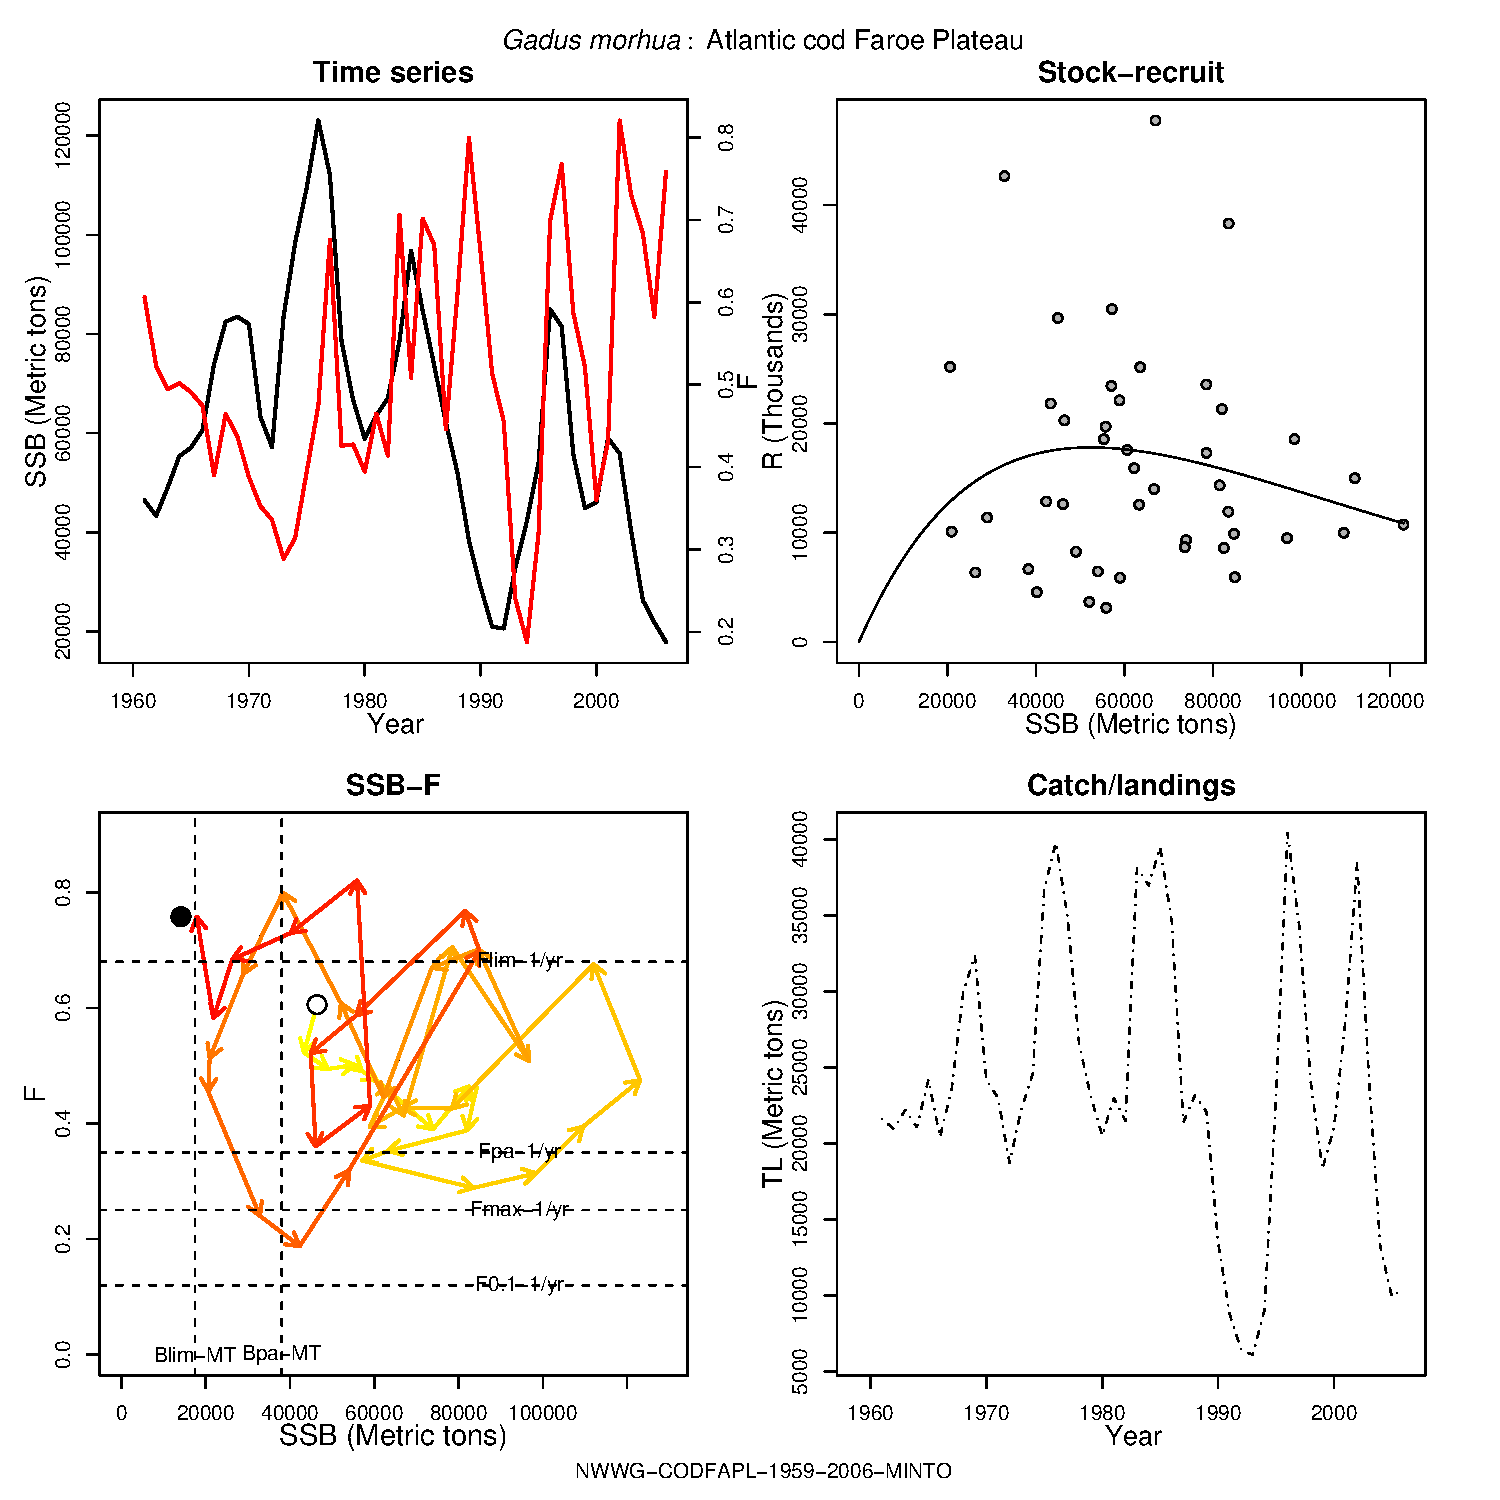
\includegraphics[width=1.2\textwidth]{../R/figures/NWWG-CODFAPL-1959-2006-MINTO.pdf}
\end{center}

\subsubsection{Gadus morhua - Atlantic cod}\index{Atlantic cod}\index{Gadus morhua}\index{Gadidae!Gadus morhua}
\begin{center}
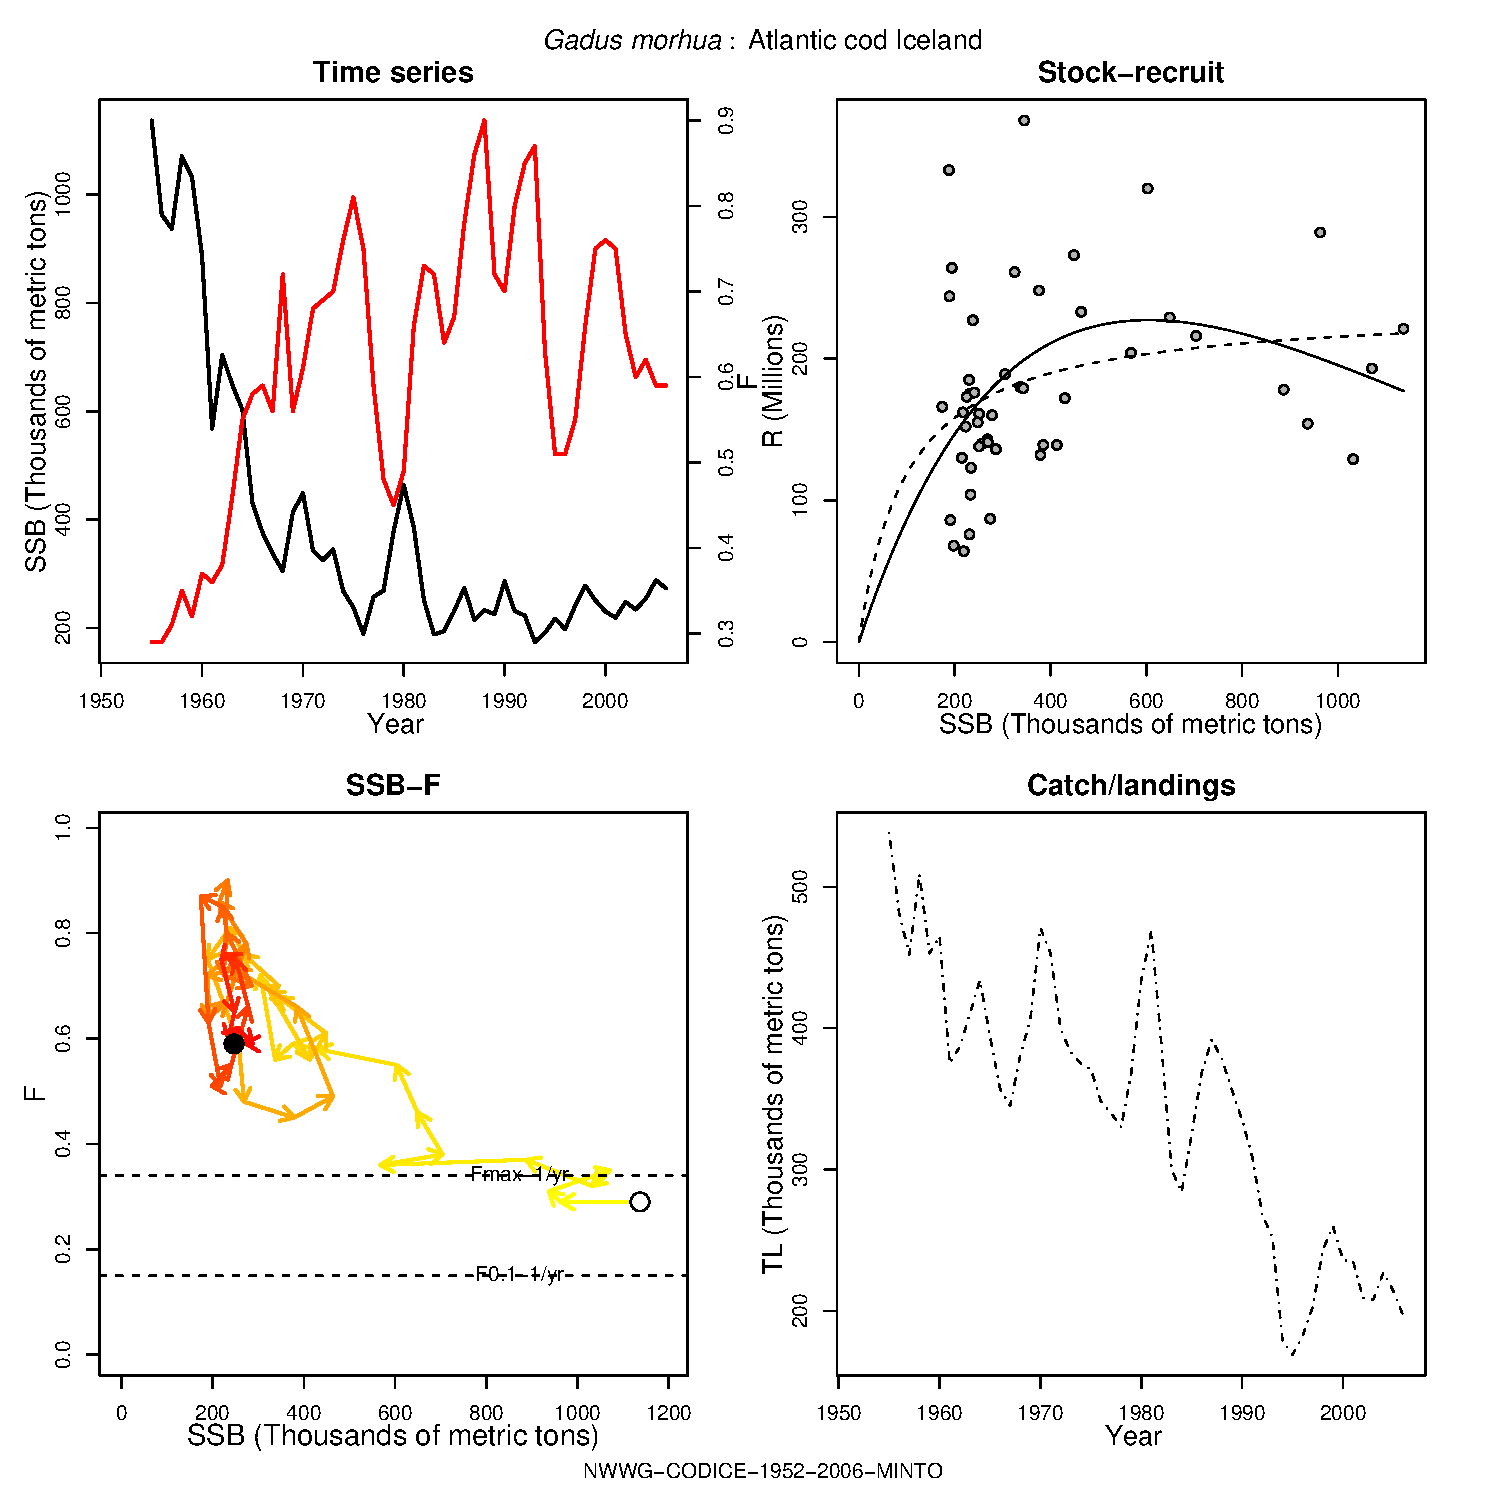
\includegraphics[width=1.2\textwidth]{../R/figures/NWWG-CODICE-1952-2006-MINTO.pdf}
\end{center}

\subsubsection{Gadus morhua - Atlantic cod}\index{Atlantic cod}\index{Gadus morhua}\index{Gadidae!Gadus morhua}
\begin{center}
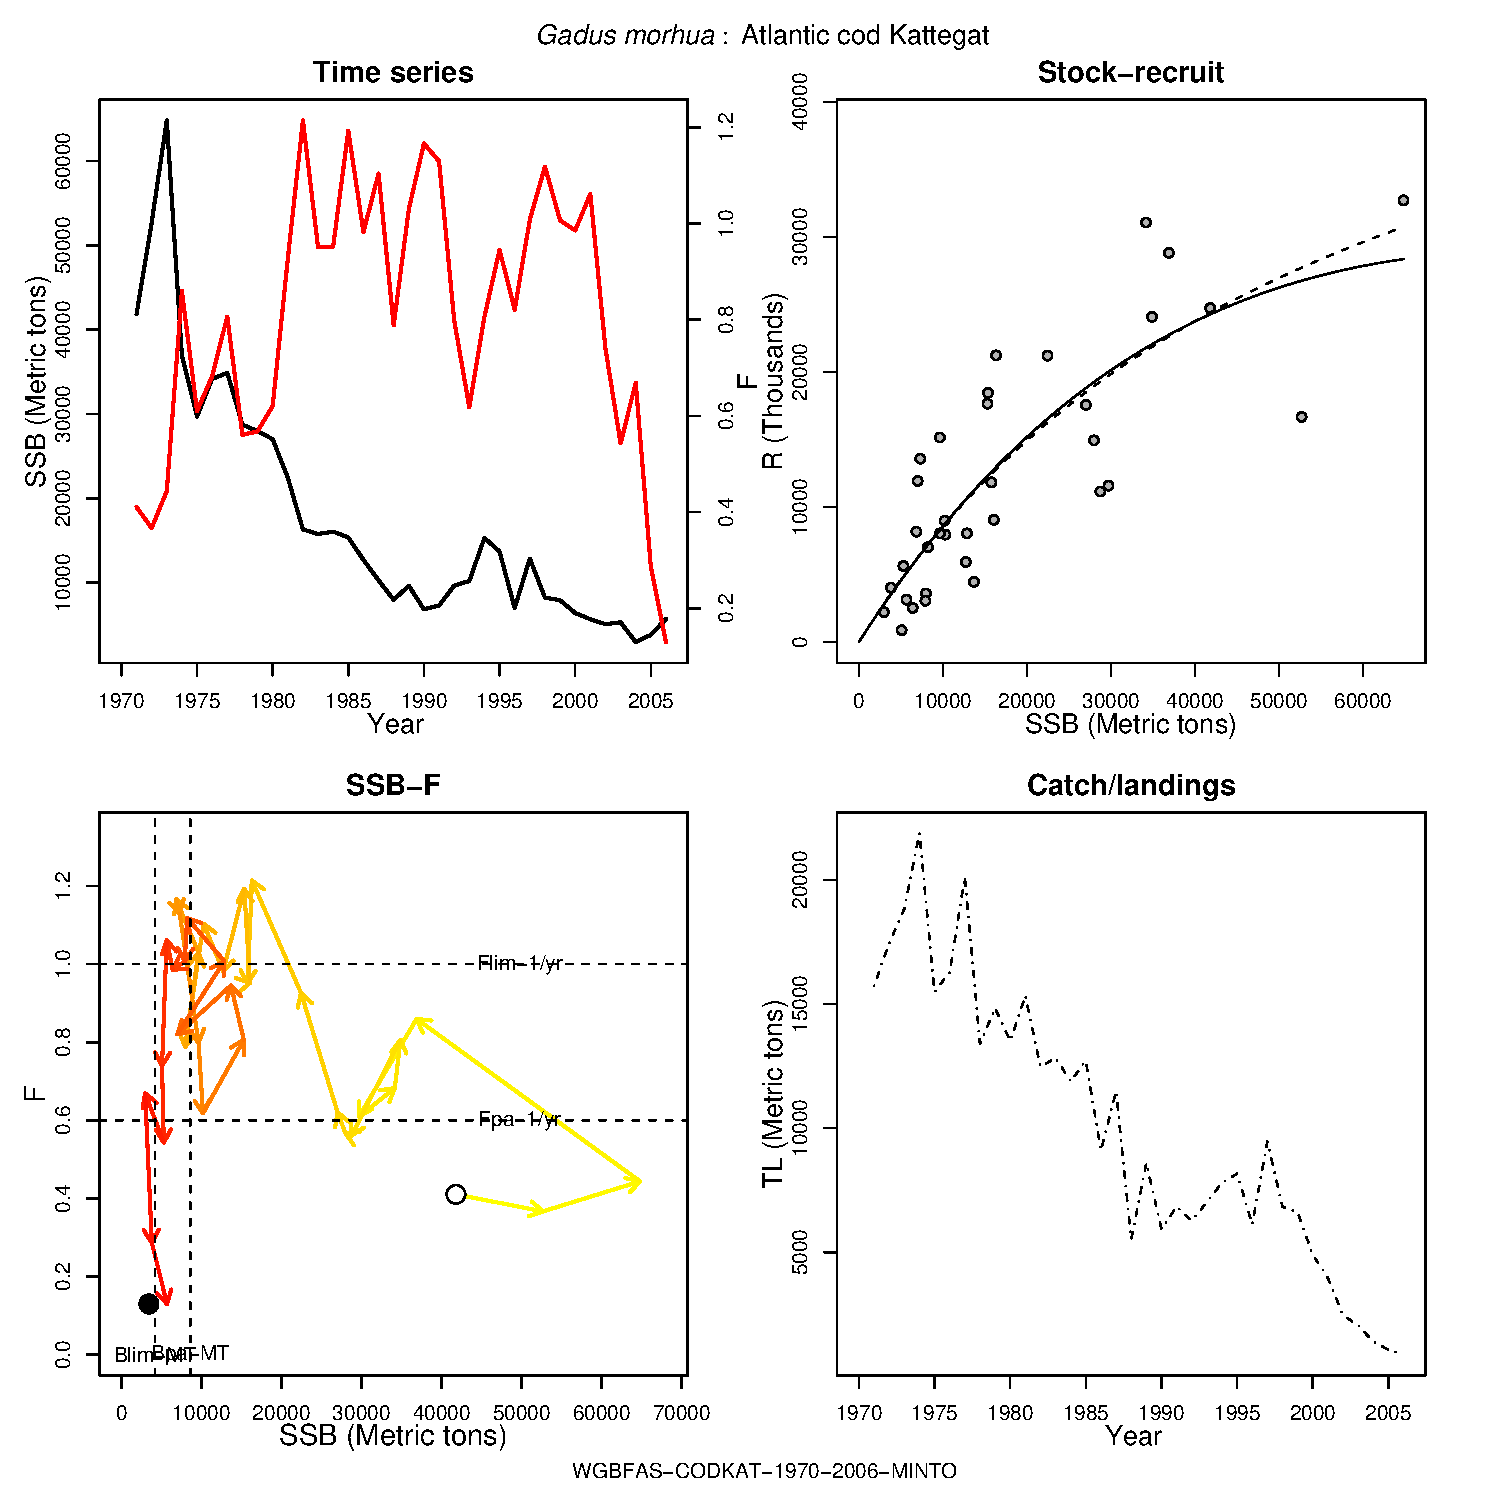
\includegraphics[width=1.2\textwidth]{../R/figures/WGBFAS-CODKAT-1970-2006-MINTO.pdf}
\end{center}

\subsubsection{Gadus morhua - Atlantic cod}\index{Atlantic cod}\index{Gadus morhua}\index{Gadidae!Gadus morhua}
\begin{center}
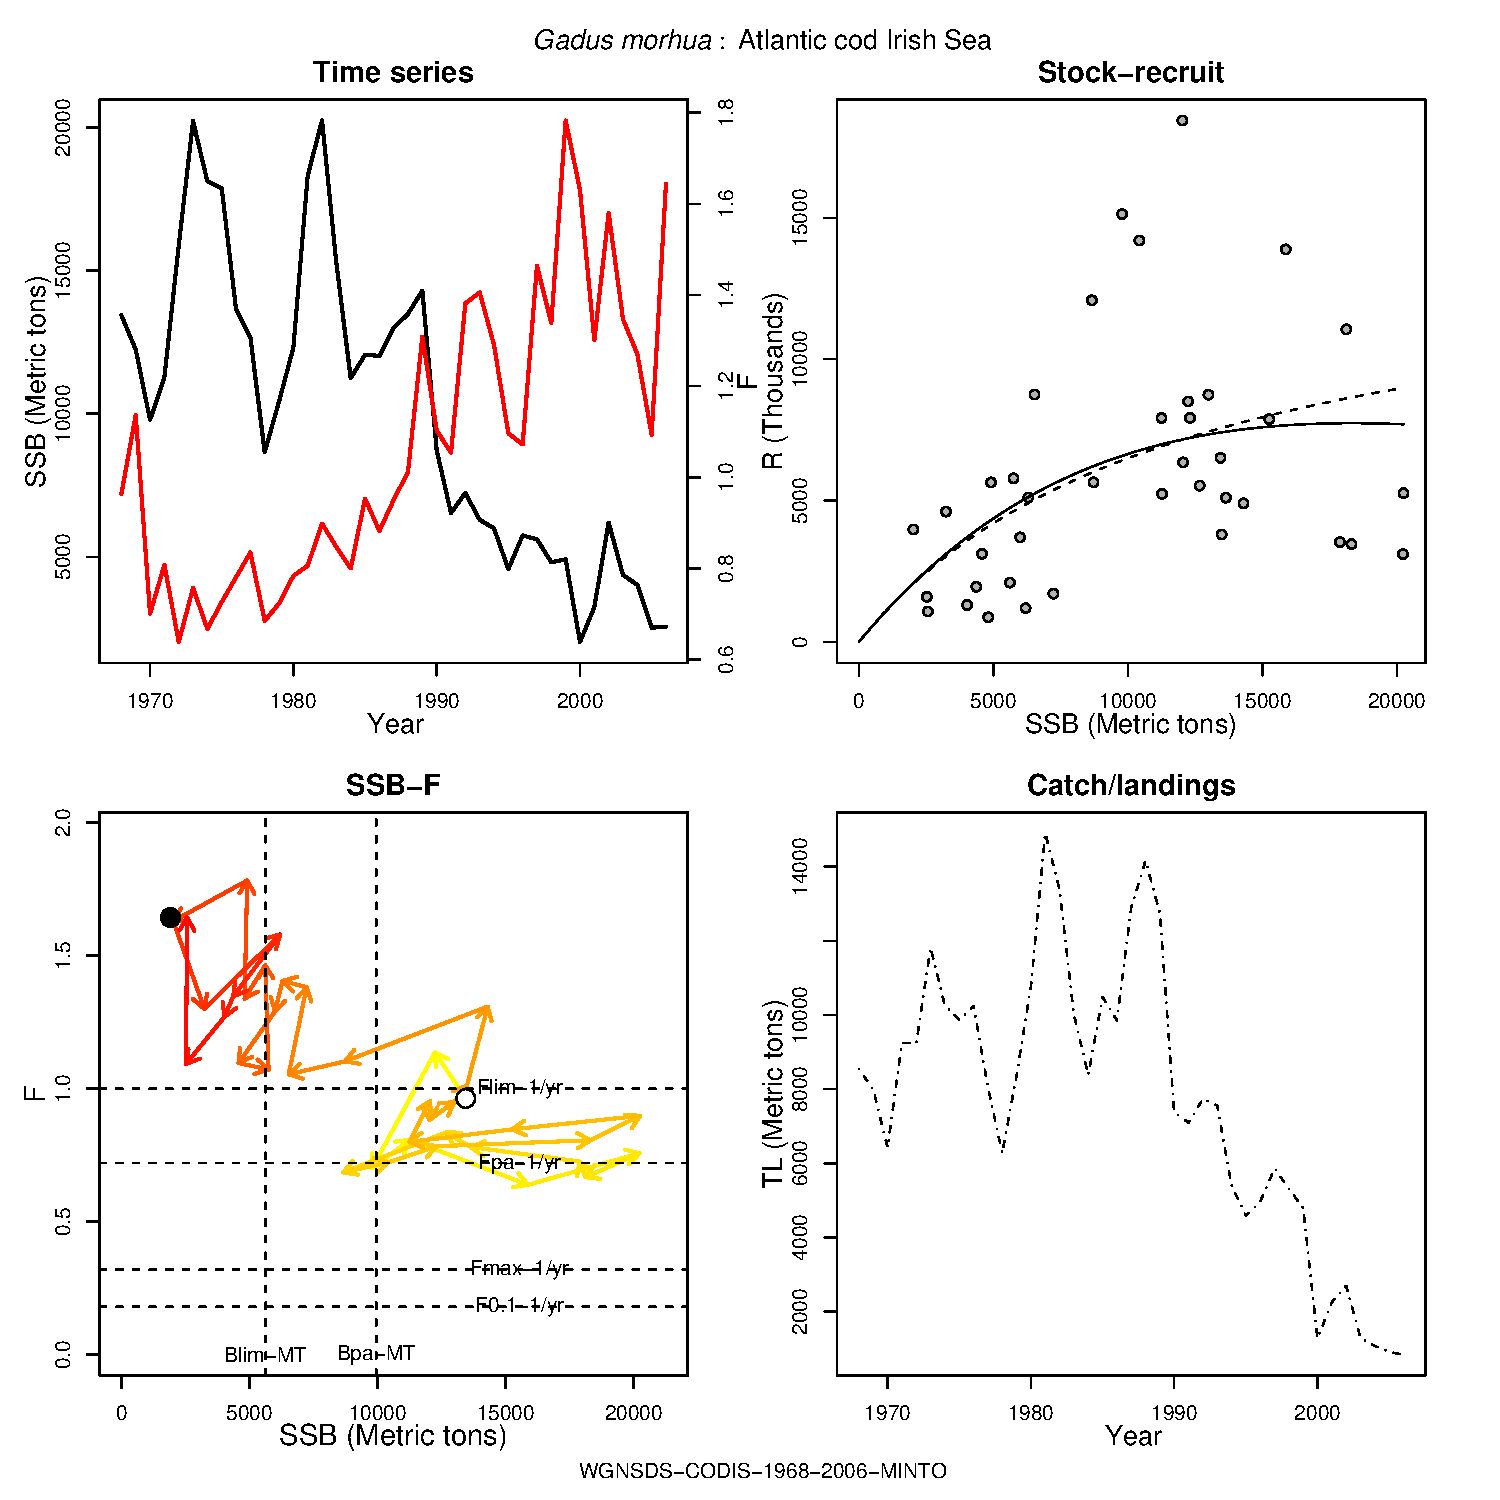
\includegraphics[width=1.2\textwidth]{../R/figures/WGNSDS-CODIS-1968-2006-MINTO.pdf}
\end{center}

\subsubsection{Gadus morhua - Atlantic cod}\index{Atlantic cod}\index{Gadus morhua}\index{Gadidae!Gadus morhua}
\begin{center}
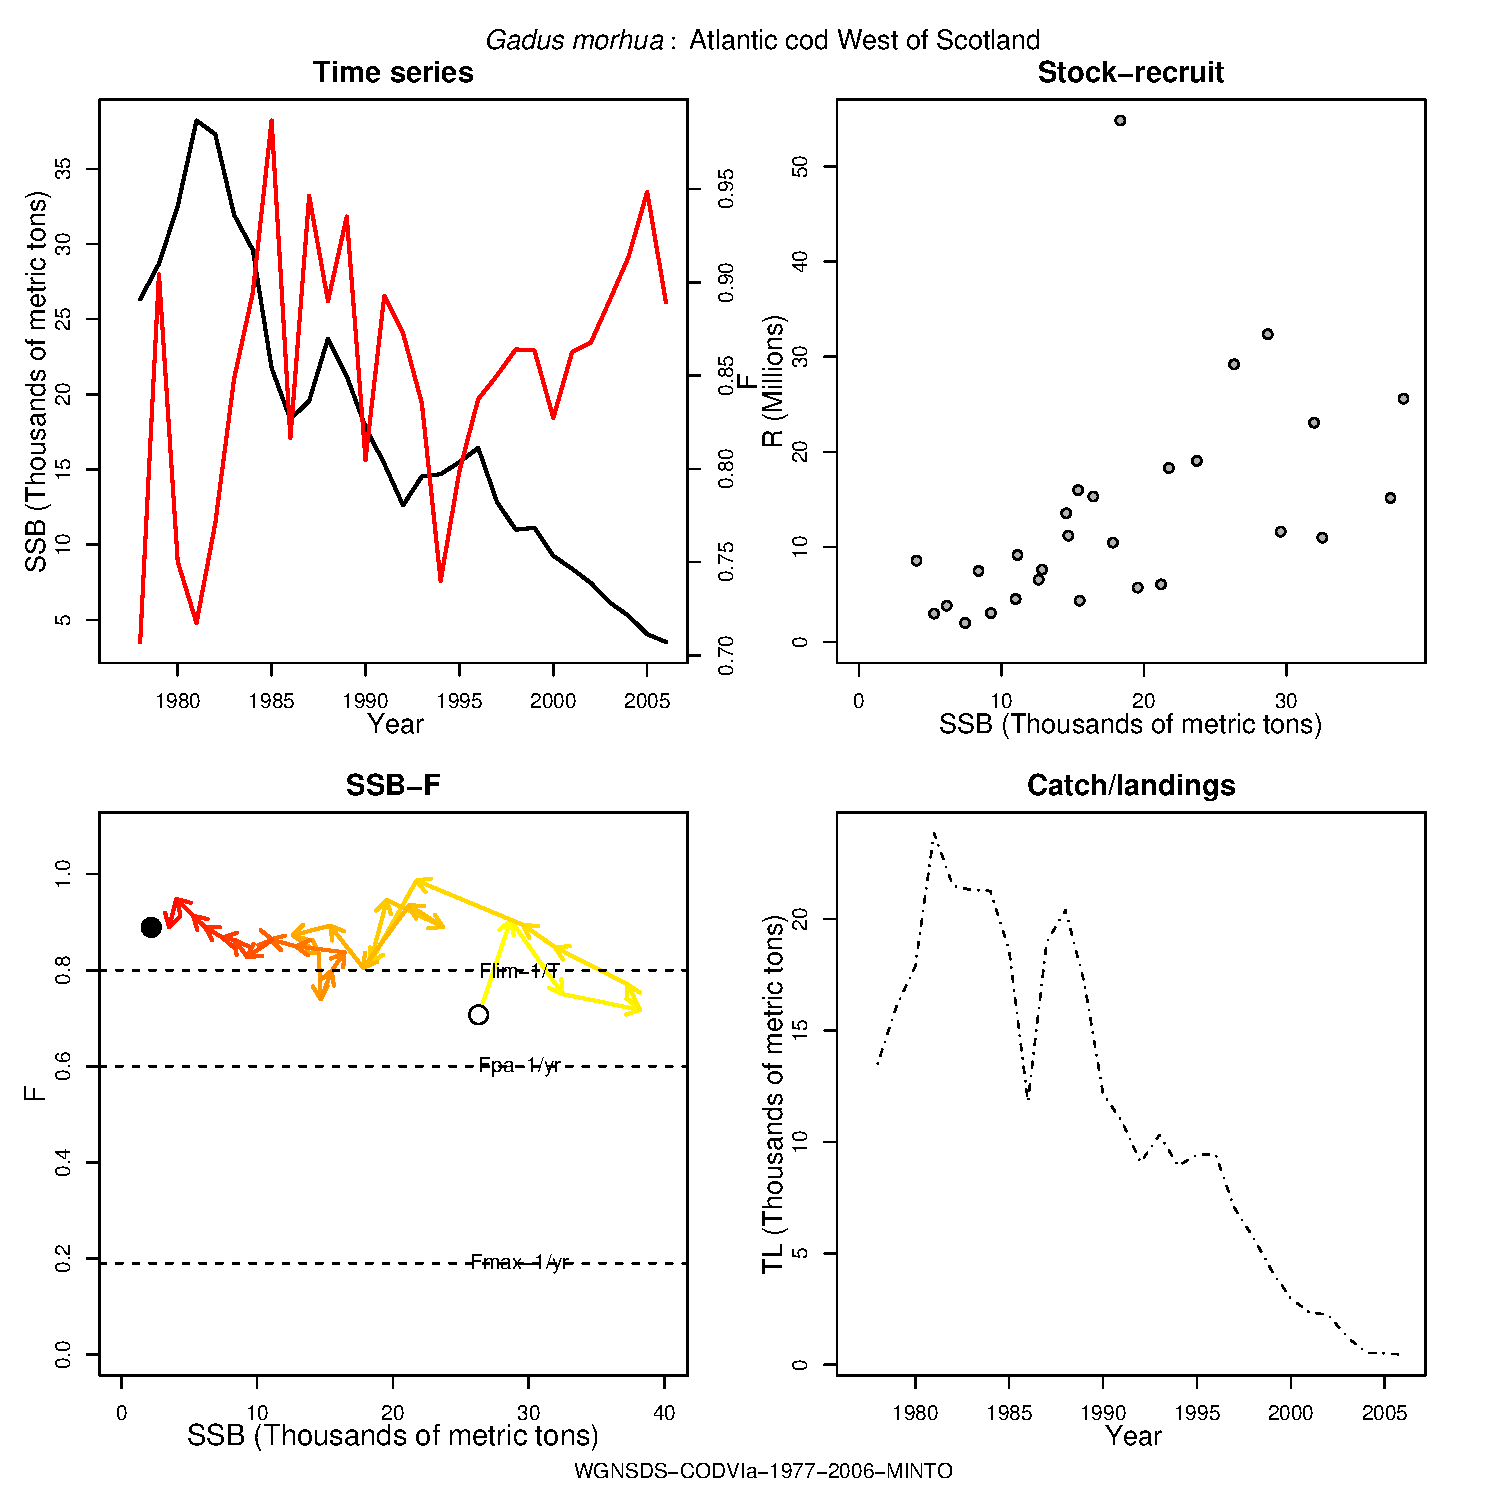
\includegraphics[width=1.2\textwidth]{../R/figures/WGNSDS-CODVIa-1977-2006-MINTO.pdf}
\end{center}

\subsubsection{Gadus morhua - Atlantic cod}\index{Atlantic cod}\index{Gadus morhua}\index{Gadidae!Gadus morhua}
\begin{center}
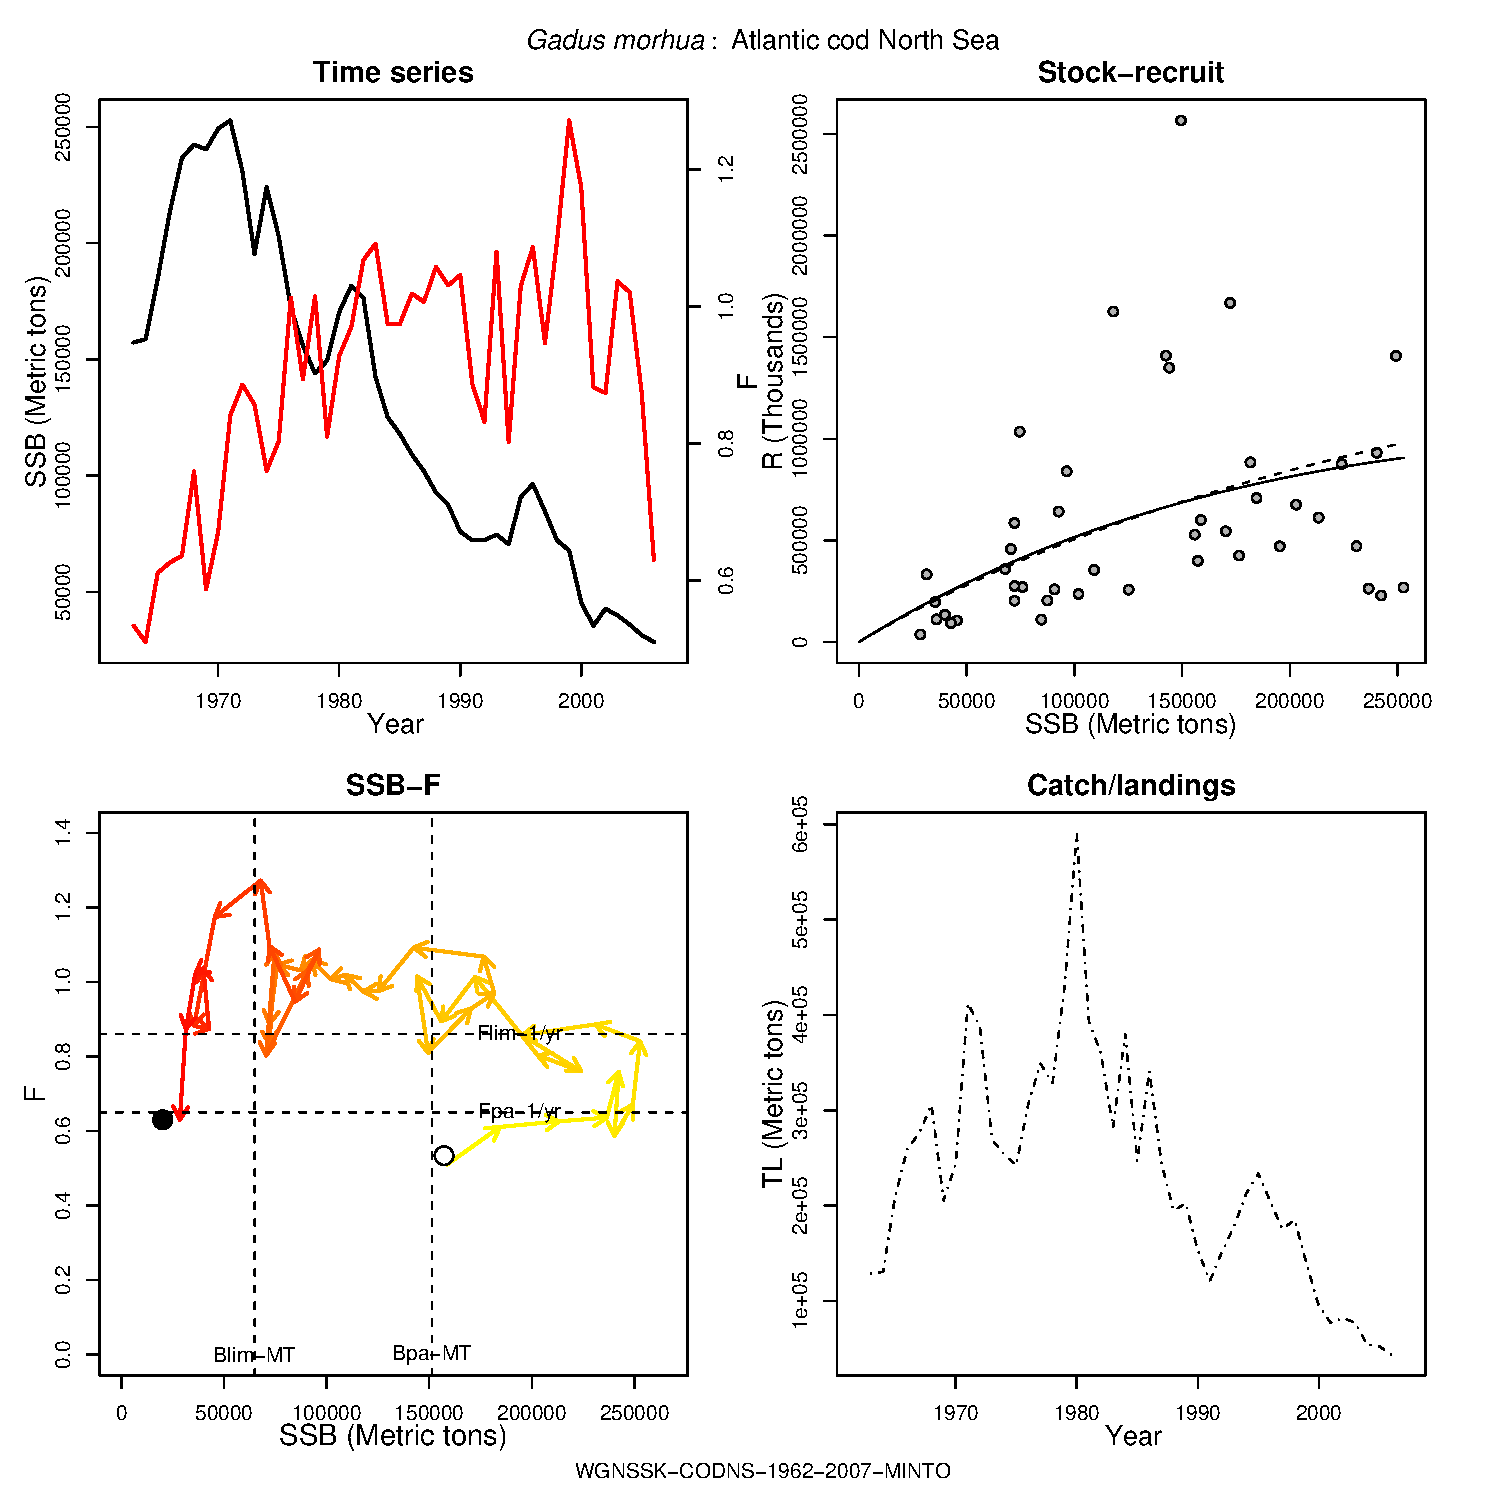
\includegraphics[width=1.2\textwidth]{../R/figures/WGNSSK-CODNS-1962-2007-MINTO.pdf}
\end{center}

\subsubsection{Gadus morhua - Atlantic cod}\index{Atlantic cod}\index{Gadus morhua}\index{Gadidae!Gadus morhua}
\begin{center}
\includegraphics[width=1.2\textwidth]{../R/figures/PHONYassessorid-COD1-1952-1992-MYERS.pdf}
\end{center}

\subsubsection{Gadus morhua - Atlantic cod}\index{Atlantic cod}\index{Gadus morhua}\index{Gadidae!Gadus morhua}
\begin{center}
\includegraphics[width=1.2\textwidth]{../R/figures/PHONYassessorid-COD2J3KL-1850-2000-MYERS.pdf}
\end{center}

\subsubsection{Gadus morhua - Atlantic cod}\index{Atlantic cod}\index{Gadus morhua}\index{Gadidae!Gadus morhua}
\begin{center}
\includegraphics[width=1.2\textwidth]{../R/figures/PHONYassessorid-COD3NO-1953-2002-MYERS.pdf}
\end{center}

\subsubsection{Gadus morhua - Atlantic cod}\index{Atlantic cod}\index{Gadus morhua}\index{Gadidae!Gadus morhua}
\begin{center}
\includegraphics[width=1.2\textwidth]{../R/figures/PHONYassessorid-COD4VsW-1957-1993-MYERS.pdf}
\end{center}

\subsubsection{Gadus morhua - Atlantic cod}\index{Atlantic cod}\index{Gadus morhua}\index{Gadidae!Gadus morhua}
\begin{center}
\includegraphics[width=1.2\textwidth]{../R/figures/PHONYassessorid-COD4X-1947-2001-MYERS.pdf}
\end{center}

\subsubsection{Gadus morhua - Atlantic cod}\index{Atlantic cod}\index{Gadus morhua}\index{Gadidae!Gadus morhua}
\begin{center}
\includegraphics[width=1.2\textwidth]{../R/figures/PHONYassessorid-COD5Z-1977-1998-MYERS.pdf}
\end{center}

\subsubsection{Gadus morhua - Atlantic cod}\index{Atlantic cod}\index{Gadus morhua}\index{Gadidae!Gadus morhua}
\begin{center}
\includegraphics[width=1.2\textwidth]{../R/figures/PHONYassessorid-CODBA2532-1964-2003-MYERS.pdf}
\end{center}

\subsubsection{Gadus morhua - Atlantic cod}\index{Atlantic cod}\index{Gadus morhua}\index{Gadidae!Gadus morhua}
\begin{center}
\includegraphics[width=1.2\textwidth]{../R/figures/PHONYassessorid-CODCOASTNOR-1982-2000-MYERS.pdf}
\end{center}

\subsubsection{Gadus morhua - Atlantic cod}\index{Atlantic cod}\index{Gadus morhua}\index{Gadidae!Gadus morhua}
\begin{center}
\includegraphics[width=1.2\textwidth]{../R/figures/PHONYassessorid-CODFAPL-1924-2000-MYERS.pdf}
\end{center}

\subsubsection{Gadus morhua - Atlantic cod}\index{Atlantic cod}\index{Gadus morhua}\index{Gadidae!Gadus morhua}
\begin{center}
\includegraphics[width=1.2\textwidth]{../R/figures/PHONYassessorid-CODICE-1905-2000-MYERS.pdf}
\end{center}

\subsubsection{Gadus morhua - Atlantic cod}\index{Atlantic cod}\index{Gadus morhua}\index{Gadidae!Gadus morhua}
\begin{center}
\includegraphics[width=1.2\textwidth]{../R/figures/PHONYassessorid-CODKAT-1970-2000-MYERS.pdf}
\end{center}

\subsubsection{Gadus morhua - Atlantic cod}\index{Atlantic cod}\index{Gadus morhua}\index{Gadidae!Gadus morhua}
\begin{center}
\includegraphics[width=1.2\textwidth]{../R/figures/PHONYassessorid-CODNEAR-1930-1991-MYERS.pdf}
\end{center}

\subsubsection{Gadus morhua - Atlantic cod}\index{Atlantic cod}\index{Gadus morhua}\index{Gadidae!Gadus morhua}
\begin{center}
\includegraphics[width=1.2\textwidth]{../R/figures/PHONYassessorid-CODNS-1930-2002-MYERS.pdf}
\end{center}

\subsubsection{Gadus morhua - Atlantic cod}\index{Atlantic cod}\index{Gadus morhua}\index{Gadidae!Gadus morhua}
\begin{center}
\includegraphics[width=1.2\textwidth]{../R/figures/PHONYassessorid-CODVIa-1965-2000-MYERS.pdf}
\end{center}

\subsubsection{Gadus morhua - Atlantic cod}\index{Atlantic cod}\index{Gadus morhua}\index{Gadidae!Gadus morhua}
\begin{center}
\includegraphics[width=1.2\textwidth]{../R/figures/DFO-COD5Zjm-1978-2003-PREFONTAINE.pdf}
\end{center}

\subsubsection{Gadus morhua - Atlantic cod}\index{Atlantic cod}\index{Gadus morhua}\index{Gadidae!Gadus morhua}
\begin{center}
\includegraphics[width=1.2\textwidth]{../R/figures/DFO-NFLD-COD2J3KLIS-1959-2006-PREFONTAINE.pdf}
\end{center}

\subsubsection{Gadus morhua - Atlantic cod}\index{Atlantic cod}\index{Gadus morhua}\index{Gadidae!Gadus morhua}
\begin{center}
\includegraphics[width=1.2\textwidth]{../R/figures/NAFO-SC-COD3NO-1953-2007-PREFONTAINE.pdf}
\end{center}

\subsubsection{Melanogrammus aeglefinus - Haddock}\index{Haddock}\index{Melanogrammus aeglefinus}\index{Gadidae!Melanogrammus aeglefinus}
\begin{center}
\includegraphics[width=1.2\textwidth]{../R/figures/NMFS-HADGB-2005-FOGARTY.pdf}
\end{center}

\subsubsection{Melanogrammus aeglefinus - Haddock}\index{Haddock}\index{Melanogrammus aeglefinus}\index{Gadidae!Melanogrammus aeglefinus}
\begin{center}
\includegraphics[width=1.2\textwidth]{../R/figures/AFWG-HADNEAR-1947-2006-MINTO.pdf}
\end{center}

\subsubsection{Melanogrammus aeglefinus - Haddock}\index{Haddock}\index{Melanogrammus aeglefinus}\index{Gadidae!Melanogrammus aeglefinus}
\begin{center}
\includegraphics[width=1.2\textwidth]{../R/figures/NWWG-HADFAPL-1955-2007-MINTO.pdf}
\end{center}

\subsubsection{Melanogrammus aeglefinus - Haddock}\index{Haddock}\index{Melanogrammus aeglefinus}\index{Gadidae!Melanogrammus aeglefinus}
\begin{center}
\includegraphics[width=1.2\textwidth]{../R/figures/NWWG-HADICE-1977-2007-MINTO.pdf}
\end{center}

\subsubsection{Melanogrammus aeglefinus - Haddock}\index{Haddock}\index{Melanogrammus aeglefinus}\index{Gadidae!Melanogrammus aeglefinus}
\begin{center}
\includegraphics[width=1.2\textwidth]{../R/figures/WGNSDS-HADIS-1991-2006-MINTO.pdf}
\end{center}

\subsubsection{Melanogrammus aeglefinus - Haddock}\index{Haddock}\index{Melanogrammus aeglefinus}\index{Gadidae!Melanogrammus aeglefinus}
\begin{center}
\includegraphics[width=1.2\textwidth]{../R/figures/WGNSDS-HADVIa-1977-2006-MINTO.pdf}
\end{center}

\subsubsection{Melanogrammus aeglefinus - Haddock}\index{Haddock}\index{Melanogrammus aeglefinus}\index{Gadidae!Melanogrammus aeglefinus}
\begin{center}
\includegraphics[width=1.2\textwidth]{../R/figures/WGNSSK-HADNS-IIIa-1963-2006-MINTO.pdf}
\end{center}

\subsubsection{Melanogrammus aeglefinus - Haddock}\index{Haddock}\index{Melanogrammus aeglefinus}\index{Gadidae!Melanogrammus aeglefinus}
\begin{center}
\includegraphics[width=1.2\textwidth]{../R/figures/PHONYassessorid-HADFAPL-1959-2000-MYERS.pdf}
\end{center}

\subsubsection{Melanogrammus aeglefinus - Haddock}\index{Haddock}\index{Melanogrammus aeglefinus}\index{Gadidae!Melanogrammus aeglefinus}
\begin{center}
\includegraphics[width=1.2\textwidth]{../R/figures/PHONYassessorid-HADICE-1950-1990-MYERS.pdf}
\end{center}

\subsubsection{Melanogrammus aeglefinus - Haddock}\index{Haddock}\index{Melanogrammus aeglefinus}\index{Gadidae!Melanogrammus aeglefinus}
\begin{center}
\includegraphics[width=1.2\textwidth]{../R/figures/PHONYassessorid-HADIS-1993-2000-MYERS.pdf}
\end{center}

\subsubsection{Melanogrammus aeglefinus - Haddock}\index{Haddock}\index{Melanogrammus aeglefinus}\index{Gadidae!Melanogrammus aeglefinus}
\begin{center}
\includegraphics[width=1.2\textwidth]{../R/figures/PHONYassessorid-HADNEAR-1947-2004-MYERS.pdf}
\end{center}

\subsubsection{Melanogrammus aeglefinus - Haddock}\index{Haddock}\index{Melanogrammus aeglefinus}\index{Gadidae!Melanogrammus aeglefinus}
\begin{center}
\includegraphics[width=1.2\textwidth]{../R/figures/PHONYassessorid-HADVIa-1965-1993-MYERS.pdf}
\end{center}

\subsubsection{Melanogrammus aeglefinus - Haddock}\index{Haddock}\index{Melanogrammus aeglefinus}\index{Gadidae!Melanogrammus aeglefinus}
\begin{center}
\includegraphics[width=1.2\textwidth]{../R/figures/DFO-HAD4X5Y-1960-2003-PREFONTAINE.pdf}
\end{center}

\subsubsection{Melanogrammus aeglefinus - Haddock}\index{Haddock}\index{Melanogrammus aeglefinus}\index{Gadidae!Melanogrammus aeglefinus}
\begin{center}
\includegraphics[width=1.2\textwidth]{../R/figures/DFO-HAD5Zejm-1969-2003-PREFONTAINE.pdf}
\end{center}

\subsubsection{Merlangius merlangus - Whiting}\index{Whiting}\index{Merlangius merlangus}\index{Gadidae!Merlangius merlangus}
\begin{center}
\includegraphics[width=1.2\textwidth]{../R/figures/WGNSDS-WHITVIa-1984-2007-MINTO.pdf}
\end{center}

\subsubsection{Merlangius merlangus - Whiting}\index{Whiting}\index{Merlangius merlangus}\index{Gadidae!Merlangius merlangus}
\begin{center}
\includegraphics[width=1.2\textwidth]{../R/figures/WGNSSK-WHITNS-VIId-IIIa-1979-2006-MINTO.pdf}
\end{center}

\subsubsection{Merlangius merlangus - Whiting}\index{Whiting}\index{Merlangius merlangus}\index{Gadidae!Merlangius merlangus}
\begin{center}
\includegraphics[width=1.2\textwidth]{../R/figures/PHONYassessorid-WHITBLACKW-1971-1993-MYERS.pdf}
\end{center}

\subsubsection{Merlangius merlangus - Whiting}\index{Whiting}\index{Merlangius merlangus}\index{Gadidae!Merlangius merlangus}
\begin{center}
\includegraphics[width=1.2\textwidth]{../R/figures/PHONYassessorid-WHITVIa-1964-1992-MYERS.pdf}
\end{center}

\subsubsection{Pollachius virens - Pollock}\index{Pollock}\index{Pollachius virens}\index{Gadidae!Pollachius virens}
\begin{center}
\includegraphics[width=1.2\textwidth]{../R/figures/AFWG-POLLNEAR-1957-2006-MINTO.pdf}
\end{center}

\subsubsection{Pollachius virens - Pollock}\index{Pollock}\index{Pollachius virens}\index{Gadidae!Pollachius virens}
\begin{center}
\includegraphics[width=1.2\textwidth]{../R/figures/NWWG-POLLFAPL-1958-2006-MINTO.pdf}
\end{center}

\subsubsection{Pollachius virens - Pollock}\index{Pollock}\index{Pollachius virens}\index{Gadidae!Pollachius virens}
\begin{center}
\includegraphics[width=1.2\textwidth]{../R/figures/WGNSSK-POLLNS-VI-IIIa-1964-2006-MINTO.pdf}
\end{center}

\subsubsection{Pollachius virens - Pollock}\index{Pollock}\index{Pollachius virens}\index{Gadidae!Pollachius virens}
\begin{center}
\includegraphics[width=1.2\textwidth]{../R/figures/PHONYassessorid-POLLNEAR-1957-2004-MYERS.pdf}
\end{center}

\subsubsection{Pollachius virens - Pollock}\index{Pollock}\index{Pollachius virens}\index{Gadidae!Pollachius virens}
\begin{center}
\includegraphics[width=1.2\textwidth]{../R/figures/DFO-POLL4VWX5Zc-1974-2007-PREFONTAINE.pdf}
\end{center}

\subsubsection{Theragra chalcogramma - Walleye pollock}\index{Walleye pollock}\index{Theragra chalcogramma}\index{Gadidae!Theragra chalcogramma}
\begin{center}
\includegraphics[width=1.2\textwidth]{../R/figures/NMFS-WPOLLGA-2007-FOGARTY.pdf}
\end{center}

\subsubsection{Trisopterus esmarkii - Norway Pout}\index{Norway Pout}\index{Trisopterus esmarkii}\index{Gadidae!Trisopterus esmarkii}
\begin{center}
\includegraphics[width=1.2\textwidth]{../R/figures/WGNSSK-NPOUTNS-1983-2007-MINTO.pdf}
\end{center}

\subsubsection{Trisopterus esmarkii - Norway Pout}\index{Norway Pout}\index{Trisopterus esmarkii}\index{Gadidae!Trisopterus esmarkii}
\begin{center}
\includegraphics[width=1.2\textwidth]{../R/figures/PHONYassessorid-NPOUTNS-1957-2001-MYERS.pdf}
\end{center}

\subsection{Merlucciidae}\index{Merlucciidae}\index{Gadiformes!Merlucciidae}

\subsubsection{Macruronus novaezelandiae - Hoki}\index{Hoki}\index{Macruronus novaezelandiae}\index{Merlucciidae!Macruronus novaezelandiae}
\begin{center}
\includegraphics[width=1.2\textwidth]{../R/figures/NIWA-HOKIENZ-1972-2007-FRANCIS.pdf}
\end{center}

\subsubsection{Macruronus novaezelandiae - Hoki}\index{Hoki}\index{Macruronus novaezelandiae}\index{Merlucciidae!Macruronus novaezelandiae}
\begin{center}
\includegraphics[width=1.2\textwidth]{../R/figures/NIWA-HOKIWNZ-1972-2007-FRANCIS.pdf}
\end{center}

\subsubsection{Merluccius productus - Pacific hake}\index{Pacific hake}\index{Merluccius productus}\index{Merlucciidae!Merluccius productus}
\begin{center}
\includegraphics[width=1.2\textwidth]{../R/figures/NMFS-PHAKEPCOAST-2006-FOGARTY.pdf}
\end{center}

\subsubsection{Merluccius productus - Pacific hake}\index{Pacific hake}\index{Merluccius productus}\index{Merlucciidae!Merluccius productus}
\begin{center}
\includegraphics[width=1.2\textwidth]{../R/figures/NMFS-PHAKEPCOAST-2007-FOGARTY.pdf}
\end{center}

\section{Lophiiformes}\index{Lophiiformes}

\subsection{Lophiidae}\index{Lophiidae}\index{Lophiiformes!Lophiidae}

\subsubsection{Lophius americanus - Monkfish}\index{Monkfish}\index{Lophius americanus}\index{Lophiidae!Lophius americanus}
\begin{center}
\includegraphics[width=1.2\textwidth]{../R/figures/NMFS-MONKGOMNGB-2007-FOGARTY.pdf}
\end{center}

\subsubsection{Lophius americanus - Monkfish}\index{Monkfish}\index{Lophius americanus}\index{Lophiidae!Lophius americanus}
\begin{center}
\includegraphics[width=1.2\textwidth]{../R/figures/NMFS-MONKSGBMATL-2007-FOGARTY.pdf}
\end{center}

\section{Ophidiiformes}\index{Ophidiiformes}

\subsection{Ophidiidae}\index{Ophidiidae}\index{Ophidiiformes!Ophidiidae}

\subsubsection{Genypterus blacodes - Australian rockling}\index{Australian rockling}\index{Genypterus blacodes}\index{Ophidiidae!Genypterus blacodes}
\begin{center}
\includegraphics[width=1.2\textwidth]{../R/figures/CSIRO-PINKLINGGABSESSF-YEAR-2007-Fulton.pdf}
\end{center}

\subsubsection{Genypterus blacodes - Australian rockling}\index{Australian rockling}\index{Genypterus blacodes}\index{Ophidiidae!Genypterus blacodes}
\begin{center}
\includegraphics[width=1.2\textwidth]{../R/figures/CSIRO-PINKLINGSESSF-YEAR-2007-Fulton.pdf}
\end{center}

\section{Osmeriformes}\index{Osmeriformes}

\subsection{Osmeridae}\index{Osmeridae}\index{Osmeriformes!Osmeridae}

\subsubsection{Mallotus villosus - Capelin}\index{Capelin}\index{Mallotus villosus}\index{Osmeridae!Mallotus villosus}
\begin{center}
\includegraphics[width=1.2\textwidth]{../R/figures/AFWG-CAPENOR-1964-2006-MINTO.pdf}
\end{center}

\subsubsection{Mallotus villosus - Capelin}\index{Capelin}\index{Mallotus villosus}\index{Osmeridae!Mallotus villosus}
\begin{center}
\includegraphics[width=1.2\textwidth]{../R/figures/NWWG-CAPEICE-1977-2007-MINTO.pdf}
\end{center}

\subsubsection{Mallotus villosus - Capelin}\index{Capelin}\index{Mallotus villosus}\index{Osmeridae!Mallotus villosus}
\begin{center}
\includegraphics[width=1.2\textwidth]{../R/figures/PHONYassessorid-CAPEICE-1977-1997-MYERS.pdf}
\end{center}

\section{Ostreoida}\index{Ostreoida}

\subsection{Pectinidae}\index{Pectinidae}\index{Ostreoida!Pectinidae}

\subsubsection{Placopecten magellanicus - Sea scallop}\index{Sea scallop}\index{Placopecten magellanicus}\index{Pectinidae!Placopecten magellanicus}
\begin{center}
\includegraphics[width=1.2\textwidth]{../R/figures/NMFS-SCALLNWATLC-2007-FOGARTY.pdf}
\end{center}

\section{Perciformes}\index{Perciformes}

\subsection{Ammodytidae}\index{Ammodytidae}\index{Perciformes!Ammodytidae}

\subsubsection{Ammodytes marinus - Sand eel}\index{Sand eel}\index{Ammodytes marinus}\index{Ammodytidae!Ammodytes marinus}
\begin{center}
\includegraphics[width=1.2\textwidth]{../R/figures/WGNSSK-SEELNS-1983-2007-MINTO.pdf}
\end{center}

\subsection{Centrolophidae}\index{Centrolophidae}\index{Perciformes!Centrolophidae}

\subsubsection{Seriolella punctata - Silverfish}\index{Silverfish}\index{Seriolella punctata}\index{Centrolophidae!Seriolella punctata}
\begin{center}
\includegraphics[width=1.2\textwidth]{../R/figures/CSIRO-SILVERFISHSESSF-YEAR-2006-Fulton.pdf}
\end{center}

\subsection{Cheilodactylidae}\index{Cheilodactylidae}\index{Perciformes!Cheilodactylidae}

\subsubsection{Nemadactylus macropterus - Hawaiian morwong}\index{Hawaiian morwong}\index{Nemadactylus macropterus}\index{Cheilodactylidae!Nemadactylus macropterus}
\begin{center}
\includegraphics[width=1.2\textwidth]{../R/figures/CSIRO-MORWONGSESSF-YEAR-2007-Fulton.pdf}
\end{center}

\subsection{Gempylidae}\index{Gempylidae}\index{Perciformes!Gempylidae}

\subsubsection{Rexea solandri - common gemfish}\index{common gemfish}\index{Rexea solandri}\index{Gempylidae!Rexea solandri}
\begin{center}
\includegraphics[width=1.2\textwidth]{../R/figures/CSIRO-GEMFISHSESSF-YEAR-2007-Fulton.pdf}
\end{center}

\subsection{Labridae}\index{Labridae}\index{Perciformes!Labridae}

\subsubsection{Tautoga onitis - Tautog}\index{Tautog}\index{Tautoga onitis}\index{Labridae!Tautoga onitis}
\begin{center}
\includegraphics[width=1.2\textwidth]{../R/figures/RIDEM-TAUTOGRI-YEAR-2007-COLLIE.pdf}
\end{center}

\subsection{Lutjanidae}\index{Lutjanidae}\index{Perciformes!Lutjanidae}

\subsubsection{Lutjanus campechanus - Red snapper}\index{Red snapper}\index{Lutjanus campechanus}\index{Lutjanidae!Lutjanus campechanus}
\begin{center}
\includegraphics[width=1.2\textwidth]{../R/figures/NMFS-RSNAPEGM-2006-FOGARTY.pdf}
\end{center}

\subsubsection{Lutjanus campechanus - Red snapper}\index{Red snapper}\index{Lutjanus campechanus}\index{Lutjanidae!Lutjanus campechanus}
\begin{center}
\includegraphics[width=1.2\textwidth]{../R/figures/NMFS-RSNAPWGM-2006-FOGARTY.pdf}
\end{center}

\subsubsection{Rhomboplites aurorubens - Vermilion snapper}\index{Vermilion snapper}\index{Rhomboplites aurorubens}\index{Lutjanidae!Rhomboplites aurorubens}
\begin{center}
\includegraphics[width=1.2\textwidth]{../R/figures/NMFS-VSNAPGM-2006-FOGARTY.pdf}
\end{center}

\subsection{Moronidae}\index{Moronidae}\index{Perciformes!Moronidae}

\subsubsection{Morone saxatilis - Striped bass}\index{Striped bass}\index{Morone saxatilis}\index{Moronidae!Morone saxatilis}
\begin{center}
\includegraphics[width=1.2\textwidth]{../R/figures/NMFS-STRIPEDBASSGOMCHATT-2008-FOGARTY.pdf}
\end{center}

\subsection{Pomatomidae}\index{Pomatomidae}\index{Perciformes!Pomatomidae}

\subsection{Scombridae}\index{Scombridae}\index{Perciformes!Scombridae}

\subsubsection{Scomberomorus cavalla - King Mackerel}\index{King Mackerel}\index{Scomberomorus cavalla}\index{Scombridae!Scomberomorus cavalla}
\begin{center}
\includegraphics[width=1.2\textwidth]{../R/figures/NMFS-KMACKGM-2004-FOGARTY.pdf}
\end{center}

\subsubsection{Scomberomorus cavalla - King Mackerel}\index{King Mackerel}\index{Scomberomorus cavalla}\index{Scombridae!Scomberomorus cavalla}
\begin{center}
\includegraphics[width=1.2\textwidth]{../R/figures/NMFS-KMACKSATLC-2004-FOGARTY.pdf}
\end{center}

\subsubsection{Scomberomorus maculatus - Spanish mackerel}\index{Spanish mackerel}\index{Scomberomorus maculatus}\index{Scombridae!Scomberomorus maculatus}
\begin{center}
\includegraphics[width=1.2\textwidth]{../R/figures/NMFS-SPANMACKGM-2003-FOGARTY.pdf}
\end{center}

\subsubsection{Scomberomorus maculatus - Spanish mackerel}\index{Spanish mackerel}\index{Scomberomorus maculatus}\index{Scombridae!Scomberomorus maculatus}
\begin{center}
\includegraphics[width=1.2\textwidth]{../R/figures/NMFS-SPANMACKSATLC-2003-FOGARTY.pdf}
\end{center}

\subsubsection{Scomber scombrus - Mackerel}\index{Mackerel}\index{Scomber scombrus}\index{Scombridae!Scomber scombrus}
\begin{center}
\includegraphics[width=1.2\textwidth]{../R/figures/NMFS-MACKGOMCHATT-2006-FOGARTY.pdf}
\end{center}

\subsubsection{Thunnus alalunga - Albacore tuna}\index{Albacore tuna}\index{Thunnus alalunga}\index{Scombridae!Thunnus alalunga}
\begin{center}
\includegraphics[width=1.2\textwidth]{../R/figures/NMFS-ALBANPAC-2006-FOGARTY.pdf}
\end{center}

\subsubsection{Thunnus albacares - Yellowfin tuna}\index{Yellowfin tuna}\index{Thunnus albacares}\index{Scombridae!Thunnus albacares}
\begin{center}
\includegraphics[width=1.2\textwidth]{../R/figures/IATTC-YFINEPAC-1975-2007-JENSEN.pdf}
\end{center}

\subsection{Sillaginidae}\index{Sillaginidae}\index{Perciformes!Sillaginidae}

\subsubsection{Sillago flindersi - School whiting}\index{School whiting}\index{Sillago flindersi}\index{Sillaginidae!Sillago flindersi}
\begin{center}
\includegraphics[width=1.2\textwidth]{../R/figures/CSIRO-SWHITSESSF-YEAR-2007-Fulton.pdf}
\end{center}

\subsection{Stromateidae}\index{Stromateidae}\index{Perciformes!Stromateidae}

\subsubsection{Peprilus triacanthus - Atlantic butterfish}\index{Atlantic butterfish}\index{Peprilus triacanthus}\index{Stromateidae!Peprilus triacanthus}
\begin{center}
\includegraphics[width=1.2\textwidth]{../R/figures/NMFS-BUTTERGOMCHATT-2004-FOGARTY.pdf}
\end{center}

\section{Pleuronectiformes}\index{Pleuronectiformes}

\subsection{Paralichthyidae}\index{Paralichthyidae}\index{Pleuronectiformes!Paralichthyidae}

\subsubsection{Paralichthys dentatus - Summer flounder}\index{Summer flounder}\index{Paralichthys dentatus}\index{Paralichthyidae!Paralichthys dentatus}
\begin{center}
\includegraphics[width=1.2\textwidth]{../R/figures/NMFS-SFLOUNMATLC-2006-FOGARTY.pdf}
\end{center}

\subsection{Pleuronectidae}\index{Pleuronectidae}\index{Pleuronectiformes!Pleuronectidae}

\subsubsection{Glyptocephalus cynoglossus - Witch flounder}\index{Witch flounder}\index{Glyptocephalus cynoglossus}\index{Pleuronectidae!Glyptocephalus cynoglossus}
\begin{center}
\includegraphics[width=1.2\textwidth]{../R/figures/NMFS-WITFLOUNNWATLC-2005-FOGARTY.pdf}
\end{center}

\subsubsection{Glyptocephalus zachirus - Rex sole}\index{Rex sole}\index{Glyptocephalus zachirus}\index{Pleuronectidae!Glyptocephalus zachirus}
\begin{center}
\includegraphics[width=1.2\textwidth]{../R/figures/NMFS-REXSOLEGA-2007-FOGARTY.pdf}
\end{center}

\subsubsection{Hippoglossoides elassodon - Flathead sole}\index{Flathead sole}\index{Hippoglossoides elassodon}\index{Pleuronectidae!Hippoglossoides elassodon}
\begin{center}
\includegraphics[width=1.2\textwidth]{../R/figures/NMFS-FLSOLEGA-2007-FOGARTY.pdf}
\end{center}

\subsubsection{Hippoglossoides platessoides - American plaice}\index{American plaice}\index{Hippoglossoides platessoides}\index{Pleuronectidae!Hippoglossoides platessoides}
\begin{center}
\includegraphics[width=1.2\textwidth]{../R/figures/NAFO-SC-AMPL3LNO-YEAR-2007-BAUM.pdf}
\end{center}

\subsubsection{Hippoglossoides platessoides - American plaice}\index{American plaice}\index{Hippoglossoides platessoides}\index{Pleuronectidae!Hippoglossoides platessoides}
\begin{center}
\includegraphics[width=1.2\textwidth]{../R/figures/NAFO-SC-AMPL3M-YEAR-2005-BAUM.pdf}
\end{center}

\subsubsection{Hippoglossoides platessoides - American plaice}\index{American plaice}\index{Hippoglossoides platessoides}\index{Pleuronectidae!Hippoglossoides platessoides}
\begin{center}
\includegraphics[width=1.2\textwidth]{../R/figures/NMFS-AMPLGOMGB-2005-FOGARTY.pdf}
\end{center}

\subsubsection{Hippoglossoides platessoides - American plaice}\index{American plaice}\index{Hippoglossoides platessoides}\index{Pleuronectidae!Hippoglossoides platessoides}
\begin{center}
\includegraphics[width=1.2\textwidth]{../R/figures/PHONYassessorid-AMPL3LNO-1958-1989-MYERS.pdf}
\end{center}

\subsubsection{Hippoglossoides platessoides - American plaice}\index{American plaice}\index{Hippoglossoides platessoides}\index{Pleuronectidae!Hippoglossoides platessoides}
\begin{center}
\includegraphics[width=1.2\textwidth]{../R/figures/NAFO-SC-AMPL3M-1960-2005-PREFONTAINE.pdf}
\end{center}

\subsubsection{Lepidopsetta polyxystra - Northern rock sole}\index{Northern rock sole}\index{Lepidopsetta polyxystra}\index{Pleuronectidae!Lepidopsetta polyxystra}
\begin{center}
\includegraphics[width=1.2\textwidth]{../R/figures/NMFS-NRSOLEEBSAI-2007-FOGARTY.pdf}
\end{center}

\subsubsection{Limanda ferruginea - Yellowtail flounder}\index{Yellowtail flounder}\index{Limanda ferruginea}\index{Pleuronectidae!Limanda ferruginea}
\begin{center}
\includegraphics[width=1.2\textwidth]{../R/figures/NMFS-YELLCCODGOM-2005-FOGARTY.pdf}
\end{center}

\subsubsection{Limanda ferruginea - Yellowtail flounder}\index{Yellowtail flounder}\index{Limanda ferruginea}\index{Pleuronectidae!Limanda ferruginea}
\begin{center}
\includegraphics[width=1.2\textwidth]{../R/figures/NMFS-YELLGB-2005-FOGARTY.pdf}
\end{center}

\subsubsection{Limanda ferruginea - Yellowtail flounder}\index{Yellowtail flounder}\index{Limanda ferruginea}\index{Pleuronectidae!Limanda ferruginea}
\begin{center}
\includegraphics[width=1.2\textwidth]{../R/figures/NMFS-YELLSNEMATL-2005-FOGARTY.pdf}
\end{center}

\subsubsection{Limanda ferruginea - Yellowtail flounder}\index{Yellowtail flounder}\index{Limanda ferruginea}\index{Pleuronectidae!Limanda ferruginea}
\begin{center}
\includegraphics[width=1.2\textwidth]{../R/figures/PHONYassessorid-YELL5Z-1960-1996-MYERS.pdf}
\end{center}

\subsubsection{Microstomus pacificus - Dover sole}\index{Dover sole}\index{Microstomus pacificus}\index{Pleuronectidae!Microstomus pacificus}
\begin{center}
\includegraphics[width=1.2\textwidth]{../R/figures/NMFS-DSOLEGA-2007-FOGARTY.pdf}
\end{center}

\subsubsection{Parophrys vetulus - English sole}\index{English sole}\index{Parophrys vetulus}\index{Pleuronectidae!Parophrys vetulus}
\begin{center}
\includegraphics[width=1.2\textwidth]{../R/figures/NMFS-ESOLEPCOAST-2007-FOGARTY.pdf}
\end{center}

\subsubsection{Pleuronectes platessa - European Plaice}\index{European Plaice}\index{Pleuronectes platessa}\index{Pleuronectidae!Pleuronectes platessa}
\begin{center}
\includegraphics[width=1.2\textwidth]{../R/figures/WGNSDS-PLAICIS-1962-2006-MINTO.pdf}
\end{center}

\subsubsection{Pleuronectes platessa - European Plaice}\index{European Plaice}\index{Pleuronectes platessa}\index{Pleuronectidae!Pleuronectes platessa}
\begin{center}
\includegraphics[width=1.2\textwidth]{../R/figures/WGNSSK-PLAIC7d-1979-2006-MINTO.pdf}
\end{center}

\subsubsection{Pleuronectes platessa - European Plaice}\index{European Plaice}\index{Pleuronectes platessa}\index{Pleuronectidae!Pleuronectes platessa}
\begin{center}
\includegraphics[width=1.2\textwidth]{../R/figures/WGNSSK-PLAICIIIa-1976-2005-MINTO.pdf}
\end{center}

\subsubsection{Pleuronectes platessa - European Plaice}\index{European Plaice}\index{Pleuronectes platessa}\index{Pleuronectidae!Pleuronectes platessa}
\begin{center}
\includegraphics[width=1.2\textwidth]{../R/figures/WGNSSK-PLAICNS-1956-2006-MINTO.pdf}
\end{center}

\subsubsection{Pleuronectes platessa - European Plaice}\index{European Plaice}\index{Pleuronectes platessa}\index{Pleuronectidae!Pleuronectes platessa}
\begin{center}
\includegraphics[width=1.2\textwidth]{../R/figures/PHONYassessorid-PLAIC7d-1979-2000-MYERS.pdf}
\end{center}

\subsubsection{Pleuronectes platessa - European Plaice}\index{European Plaice}\index{Pleuronectes platessa}\index{Pleuronectidae!Pleuronectes platessa}
\begin{center}
\includegraphics[width=1.2\textwidth]{../R/figures/PHONYassessorid-PLAICIIIa-1976-2001-MYERS.pdf}
\end{center}

\subsubsection{Pleuronectes platessa - European Plaice}\index{European Plaice}\index{Pleuronectes platessa}\index{Pleuronectidae!Pleuronectes platessa}
\begin{center}
\includegraphics[width=1.2\textwidth]{../R/figures/PHONYassessorid-PLAICIS-1963-2000-MYERS.pdf}
\end{center}

\subsubsection{Pleuronectes platessa - European Plaice}\index{European Plaice}\index{Pleuronectes platessa}\index{Pleuronectidae!Pleuronectes platessa}
\begin{center}
\includegraphics[width=1.2\textwidth]{../R/figures/PHONYassessorid-PLAICNS-1956-2000-MYERS.pdf}
\end{center}

\subsubsection{Pseudopleuronectes americanus - Winter flounder}\index{Winter flounder}\index{Pseudopleuronectes americanus}\index{Pleuronectidae!Pseudopleuronectes americanus}
\begin{center}
\includegraphics[width=1.2\textwidth]{../R/figures/RIDEM-WINFLOUNDRI-YEAR-2007-COLLIE.pdf}
\end{center}

\subsubsection{Pseudopleuronectes americanus - Winter flounder}\index{Winter flounder}\index{Pseudopleuronectes americanus}\index{Pleuronectidae!Pseudopleuronectes americanus}
\begin{center}
\includegraphics[width=1.2\textwidth]{../R/figures/NMFS-WINFLOUNGOM-2005-FOGARTY.pdf}
\end{center}

\subsubsection{Pseudopleuronectes americanus - Winter flounder}\index{Winter flounder}\index{Pseudopleuronectes americanus}\index{Pleuronectidae!Pseudopleuronectes americanus}
\begin{center}
\includegraphics[width=1.2\textwidth]{../R/figures/NMFS-WINFLOUNSNEMATL-2005-FOGARTY.pdf}
\end{center}

\subsubsection{Reinhardtius hippoglossoides - Greenland halibut}\index{Greenland halibut}\index{Reinhardtius hippoglossoides}\index{Pleuronectidae!Reinhardtius hippoglossoides}
\begin{center}
\includegraphics[width=1.2\textwidth]{../R/figures/AFWG-GHALNEAR-1959-2006-MINTO.pdf}
\end{center}

\subsubsection{Reinhardtius hippoglossoides - Greenland halibut}\index{Greenland halibut}\index{Reinhardtius hippoglossoides}\index{Pleuronectidae!Reinhardtius hippoglossoides}
\begin{center}
\includegraphics[width=1.2\textwidth]{../R/figures/PHONYassessorid-GHALNEAR-1959-2004-MYERS.pdf}
\end{center}

\subsubsection{Reinhardtius hippoglossoides - Greenland halibut}\index{Greenland halibut}\index{Reinhardtius hippoglossoides}\index{Pleuronectidae!Reinhardtius hippoglossoides}
\begin{center}
\includegraphics[width=1.2\textwidth]{../R/figures/NAFO-SC-GHAL23KLMNO-1960-2006-PREFONTAINE.pdf}
\end{center}

\subsubsection{Reinhardtius stomias - Arrowtooth flounder}\index{Arrowtooth flounder}\index{Reinhardtius stomias}\index{Pleuronectidae!Reinhardtius stomias}
\begin{center}
\includegraphics[width=1.2\textwidth]{../R/figures/NMFS-ARFLOUNDGA-2007-FOGARTY.pdf}
\end{center}

\subsubsection{Reinhardtius stomias - Arrowtooth flounder}\index{Arrowtooth flounder}\index{Reinhardtius stomias}\index{Pleuronectidae!Reinhardtius stomias}
\begin{center}
\includegraphics[width=1.2\textwidth]{../R/figures/NMFS-ARFLOUNDPCOAST-2007-FOGARTY.pdf}
\end{center}

\subsection{Soleidae}\index{Soleidae}\index{Pleuronectiformes!Soleidae}

\subsubsection{Solea vulgaris - common European sole}\index{common European sole}\index{Solea vulgaris}\index{Soleidae!Solea vulgaris}
\begin{center}
\includegraphics[width=1.2\textwidth]{../R/figures/WGNSDS-SOLEIS-1968-2006-MINTO.pdf}
\end{center}

\subsubsection{Solea vulgaris - common European sole}\index{common European sole}\index{Solea vulgaris}\index{Soleidae!Solea vulgaris}
\begin{center}
\includegraphics[width=1.2\textwidth]{../R/figures/WGNSSK-SOLENS-1956-2006-MINTO.pdf}
\end{center}

\subsubsection{Solea vulgaris - common European sole}\index{common European sole}\index{Solea vulgaris}\index{Soleidae!Solea vulgaris}
\begin{center}
\includegraphics[width=1.2\textwidth]{../R/figures/WGNSSK-SOLEVIId-1981-2006-MINTO.pdf}
\end{center}

\subsubsection{Solea vulgaris - common European sole}\index{common European sole}\index{Solea vulgaris}\index{Soleidae!Solea vulgaris}
\begin{center}
\includegraphics[width=1.2\textwidth]{../R/figures/PHONYassessorid-SOLEIS-1968-2000-MYERS.pdf}
\end{center}

\subsubsection{Solea vulgaris - common European sole}\index{common European sole}\index{Solea vulgaris}\index{Soleidae!Solea vulgaris}
\begin{center}
\includegraphics[width=1.2\textwidth]{../R/figures/PHONYassessorid-SOLENS-1906-2000-MYERS.pdf}
\end{center}

\subsubsection{Solea vulgaris - common European sole}\index{common European sole}\index{Solea vulgaris}\index{Soleidae!Solea vulgaris}
\begin{center}
\includegraphics[width=1.2\textwidth]{../R/figures/PHONYassessorid-SOLEVIId-1970-2000-MYERS.pdf}
\end{center}

\section{Rajiformes}\index{Rajiformes}

\subsection{Rajidae}\index{Rajidae}\index{Rajiformes!Rajidae}

\subsubsection{Raja rhina - Longnose skate}\index{Longnose skate}\index{Raja rhina}\index{Rajidae!Raja rhina}
\begin{center}
\includegraphics[width=1.2\textwidth]{../R/figures/NMFS-LNOSESKAPCOAST-2007-FOGARTY.pdf}
\end{center}

\section{Scorpaeniformes}\index{Scorpaeniformes}

\subsection{Anoplopomatidae}\index{Anoplopomatidae}\index{Scorpaeniformes!Anoplopomatidae}

\subsubsection{Anoplopoma fimbria - Sablefish}\index{Sablefish}\index{Anoplopoma fimbria}\index{Anoplopomatidae!Anoplopoma fimbria}
\begin{center}
\includegraphics[width=1.2\textwidth]{../R/figures/NMFS-SABLEFPCOAST-2007-FOGARTY.pdf}
\end{center}

\subsection{Platycephalidae}\index{Platycephalidae}\index{Scorpaeniformes!Platycephalidae}

\subsubsection{Neoplatycephalus richardsoni - Tiger flathead}\index{Tiger flathead}\index{Neoplatycephalus richardsoni}\index{Platycephalidae!Neoplatycephalus richardsoni}
\begin{center}
\includegraphics[width=1.2\textwidth]{../R/figures/CSIRO-TIGERFLATSESSF-YEAR-2006-Fulton.pdf}
\end{center}

\subsection{Scorpaenidae}\index{Scorpaenidae}\index{Scorpaeniformes!Scorpaenidae}

\subsubsection{Sebastes aleutianus - Rougheye rockfish}\index{Rougheye rockfish}\index{Sebastes aleutianus}\index{Scorpaenidae!Sebastes aleutianus}
\begin{center}
\includegraphics[width=1.2\textwidth]{../R/figures/NMFS-REYEROCKGA-2007-FOGARTY.pdf}
\end{center}

\subsubsection{Sebastes alutus - Pacific ocean perch}\index{Pacific ocean perch}\index{Sebastes alutus}\index{Scorpaenidae!Sebastes alutus}
\begin{center}
\includegraphics[width=1.2\textwidth]{../R/figures/NMFS-POPERCHPCOAST-2007-FOGARTY.pdf}
\end{center}

\subsubsection{Sebastes ciliatus - Dusky rockfish}\index{Dusky rockfish}\index{Sebastes ciliatus}\index{Scorpaenidae!Sebastes ciliatus}
\begin{center}
\includegraphics[width=1.2\textwidth]{../R/figures/NMFS-DUSKYROCKGA-2007-FOGARTY.pdf}
\end{center}

\subsubsection{Sebastes crameri - Darkblotched rockfish}\index{Darkblotched rockfish}\index{Sebastes crameri}\index{Scorpaenidae!Sebastes crameri}
\begin{center}
\includegraphics[width=1.2\textwidth]{../R/figures/NMFS-DKROCKPCOAST-2007-FOGARTY.pdf}
\end{center}

\subsubsection{Sebastes entomelas - Widow rockfish}\index{Widow rockfish}\index{Sebastes entomelas}\index{Scorpaenidae!Sebastes entomelas}
\begin{center}
\includegraphics[width=1.2\textwidth]{../R/figures/NMFS-WROCKPCOAST-2007-FOGARTY.pdf}
\end{center}

\subsubsection{Sebastes fasciatus - Acadian redfish}\index{Acadian redfish}\index{Sebastes fasciatus}\index{Scorpaenidae!Sebastes fasciatus}
\begin{center}
\includegraphics[width=1.2\textwidth]{../R/figures/NMFS-ACADREDGOMGB-2005-FOGARTY.pdf}
\end{center}

\subsubsection{Sebastes goodei - Chilipepper rockfish}\index{Chilipepper rockfish}\index{Sebastes goodei}\index{Scorpaenidae!Sebastes goodei}
\begin{center}
\includegraphics[width=1.2\textwidth]{../R/figures/NMFS-CHILISPCOAST-2007-FOGARTY.pdf}
\end{center}

\subsubsection{Sebastes levis - Cowcod}\index{Cowcod}\index{Sebastes levis}\index{Scorpaenidae!Sebastes levis}
\begin{center}
\includegraphics[width=1.2\textwidth]{../R/figures/NMFS-COWCODSCAL-2007-FOGARTY.pdf}
\end{center}

\subsubsection{Sebastes melanops - Black rockfish}\index{Black rockfish}\index{Sebastes melanops}\index{Scorpaenidae!Sebastes melanops}
\begin{center}
\includegraphics[width=1.2\textwidth]{../R/figures/NMFS-BLACKROCKNPCOAST-2007-FOGARTY.pdf}
\end{center}

\subsubsection{Sebastes mentella - Deepwater redfish}\index{Deepwater redfish}\index{Sebastes mentella}\index{Scorpaenidae!Sebastes mentella}
\begin{center}
\includegraphics[width=1.2\textwidth]{../R/figures/AFWG-REDDEEPI_II-1987-2007-MINTO.pdf}
\end{center}

\subsubsection{Sebastes mystinus - Blue rockfish}\index{Blue rockfish}\index{Sebastes mystinus}\index{Scorpaenidae!Sebastes mystinus}
\begin{center}
\includegraphics[width=1.2\textwidth]{../R/figures/NMFS-BLUEROCKCAL-2007-FOGARTY.pdf}
\end{center}

\subsubsection{Sebastes norvegicus - Golden Redfish}\index{Golden Redfish}\index{Sebastes norvegicus}\index{Scorpaenidae!Sebastes norvegicus}
\begin{center}
\includegraphics[width=1.2\textwidth]{../R/figures/AFWG-GOLDREDNEAR-1986-2006-MINTO.pdf}
\end{center}

\subsubsection{Sebastes paucispinis - Bocaccio}\index{Bocaccio}\index{Sebastes paucispinis}\index{Scorpaenidae!Sebastes paucispinis}
\begin{center}
\includegraphics[width=1.2\textwidth]{../R/figures/NMFS-BOCACCSPCOAST-2007-FOGARTY.pdf}
\end{center}

\subsubsection{Sebastes pinniger - Canary rockfish}\index{Canary rockfish}\index{Sebastes pinniger}\index{Scorpaenidae!Sebastes pinniger}
\begin{center}
\includegraphics[width=1.2\textwidth]{../R/figures/NMFS-CROCKPCOAST-2007-FOGARTY.pdf}
\end{center}

\subsubsection{Sebastes polyspinis - Northern rockfish}\index{Northern rockfish}\index{Sebastes polyspinis}\index{Scorpaenidae!Sebastes polyspinis}
\begin{center}
\includegraphics[width=1.2\textwidth]{../R/figures/NMFS-NROCKGA-2007-FOGARTY.pdf}
\end{center}

\subsubsection{Sebastes ruberrimus - Yelloweye rockfish}\index{Yelloweye rockfish}\index{Sebastes ruberrimus}\index{Scorpaenidae!Sebastes ruberrimus}
\begin{center}
\includegraphics[width=1.2\textwidth]{../R/figures/NMFS-YEYEROCKPCOAST-2007-FOGARTY.pdf}
\end{center}

\section{Tetraodontiformes}\index{Tetraodontiformes}

\subsection{Balistidae}\index{Balistidae}\index{Tetraodontiformes!Balistidae}

\subsubsection{Balistes capriscus - Gray triggerfish}\index{Gray triggerfish}\index{Balistes capriscus}\index{Balistidae!Balistes capriscus}
\begin{center}
\includegraphics[width=1.2\textwidth]{../R/figures/NMFS-GTRIGGM-2006-FOGARTY.pdf}
\end{center}

